%%%%%%%%%%%%%%%%%%%%%%%%%%%%%%%%%%%%%%%%%%%%%%%%%%%%%%%%%%%%%%%
%% OXFORD THESIS TEMPLATE

% Use this template to produce a standard thesis that meets the Oxford University requirements for DPhil submission
%
% Originally by Keith A. Gillow (gillow@maths.ox.ac.uk), 1997
% Modified by Sam Evans (sam@samuelevansresearch.org), 2007
% Modified by John McManigle (john@oxfordechoes.com), 2015
%
% This version Copyright (c) 2015-2017 John McManigle
%
% Broad permissions are granted to use, modify, and distribute this software
% as specified in the MIT License included in this distribution's LICENSE file.
%

% I've (John) tried to comment this file extensively, so read through it to see how to use the various options.  Remember
% that in LaTeX, any line starting with a % is NOT executed.  Several places below, you have a choice of which line to use
% out of multiple options (eg draft vs final, for PDF vs for binding, etc.)  When you pick one, add a % to the beginning of
% the lines you don't want.


%%%%% CHOOSE PAGE LAYOUT
% The most common choices should be below.  You can also do other things, like replacing "a4paper" with "letterpaper", etc.

% This one will format for two-sided binding (ie left and right pages have mirror margins; blank pages inserted where needed):
% \documentclass[a4paper,twoside]{ociamthesis}
% This one will format for one-sided binding (ie left margin > right margin; no extra blank pages):
%\documentclass[a4paper]{ociamthesis}
% This one will format for PDF output (ie equal margins, no extra blank pages):
\documentclass[a4paper,nobind,12pt]{ociamthesis} 

%

%%%%% SELECT YOUR DRAFT OPTIONS
% Three options going on here; use in any combination.  But remember to turn the first two off before
% generating a PDF to send to the printer!

% This adds a "DRAFT" footer to every normal page.  (The first page of each chapter is not a "normal" page.)
\fancyfoot[C]{\emph{Version from \today}}  

% This highlights (in blue) corrections marked with (for words) \mccorrect{blah} or (for whole
% paragraphs) \begin{mccorrection} . . . \end{mccorrection}.  This can be useful for sending a PDF of
% your corrected thesis to your examiners for review.  Turn it off, and the blue disappears.
\correctionstrue


%%%%% BIBLIOGRAPHY SETUP
% Note that your bibliography will require some tweaking depending on your department, preferred format, etc.
% The options included below are just very basic "sciencey" and "humanitiesey" options to get started.
% If you've not used LaTeX before, I recommend reading a little about biblatex/biber and getting started with it.
% If you're already a LaTeX pro and are used to natbib or something, modify as necessary.
% Either way, you'll have to choose and configure an appropriate bibliography format...

% The science-type option: numerical in-text citation with references in order of appearance.
\usepackage[style=numeric-comp, sorting=none, backend=biber, doi=false, isbn=false]{biblatex}
\newcommand*{\bibtitle}{References}

% The humanities-type option: author-year in-text citation with an alphabetical works cited.
%\usepackage[style=authoryear, sorting=nyt, backend=biber, maxcitenames=2, useprefix, doi=false, isbn=false]{biblatex}
%\newcommand*{\bibtitle}{Works Cited}

% This makes the bibliography left-aligned (not 'justified') and slightly smaller font.
\renewcommand*{\bibfont}{\raggedright\small}

% Change this to the name of your .bib file (usually exported from a citation manager like Zotero or EndNote).
\addbibresource{references.bib}


% Uncomment this if you want equation numbers per section (2.3.12), instead of per chapter (2.18):
%\numberwithin{equation}{subsection}



%%%%% THESIS / TITLE PAGE INFORMATION
% Everybody needs to complete the following:
\title{Suitably impressive thesis title}
\author{1044935}
\college{St Cross College}

% Master's candidates who require the alternate title page (with candidate number and word count)
% must also un-comment and complete the following three lines:
%\masterssubmission true
\candidateno{1044935}
%\wordcount{28,815}

% Uncomment the following line if your degree also includes exams (eg most masters):
\renewcommand{\submittedtext}{Submitted in partial completion of the}
% Your full degree name.  (But remember that DPhils aren't "in" anything.  They're just DPhils.)
\degree{MSc in Computer Science}
% Term and year of submission, or date if your board requires (eg most masters)
\degreedate{Trinity 2020}


%%%%% YOUR OWN PERSONAL MACROS
% This is a good place to dump your own LaTeX macros as they come up.
\usepackage{graphicx}
\usepackage{amsmath}
\usepackage{hyperref}


% To make text superscripts shortcuts
	\renewcommand{\th}{\textsuperscript{th}} % ex: I won 4\th place
	\newcommand{\nd}{\textsuperscript{nd}}
	\renewcommand{\st}{\textsuperscript{st}}
	\newcommand{\rd}{\textsuperscript{rd}}

%%%%% THE ACTUAL DOCUMENT STARTS HERE
\begin{document}



%\begin{figure}
%	\centering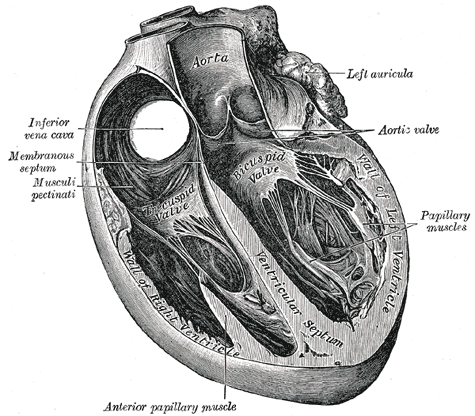
\includegraphics[width=0.7\textwidth]{figures/sample/Gray498.png} 
%	\caption[Four-chamber illustration of the human heart.]{Four-chamber illustration of the human heart.  Clockwise from upper-left: right atrium, left atrium, left ventricle, right ventricle.}
%	\label{fig:fourchamber}
%\end{figure}





%%%%% CHOOSE YOUR LINE SPACING HERE
% This is the official option.  Use it for your submission copy and library copy:
\setlength{\textbaselineskip}{22pt plus2pt}
% This is closer spacing (about 1.5-spaced) that you might prefer for your personal copies:
%\setlength{\textbaselineskip}{18pt plus2pt minus1pt}

% You can set the spacing here for the roman-numbered pages (acknowledgements, table of contents, etc.)
\setlength{\frontmatterbaselineskip}{17pt plus1pt minus1pt}

% Leave this line alone; it gets things started for the real document.
\setlength{\baselineskip}{\textbaselineskip}


%%%%% CHOOSE YOUR SECTION NUMBERING DEPTH HERE
% You have two choices.  First, how far down are sections numbered?  (Below that, they're named but
% don't get numbers.)  Second, what level of section appears in the table of contents?  These don't have
% to match: you can have numbered sections that don't show up in the ToC, or unnumbered sections that
% do.  Throughout, 0 = chapter; 1 = section; 2 = subsection; 3 = subsubsection, 4 = paragraph...

% The level that gets a number:
\setcounter{secnumdepth}{2}
% The level that shows up in the ToC:
\setcounter{tocdepth}{2}


%%%%% ABSTRACT SEPARATE
% This is used to create the separate, one-page abstract that you are required to hand into the Exam
% Schools.  You can comment it out to generate a PDF for printing or whatnot.
\begin{abstractseparate}
	%Move 1: Background to the Dissertation
%Move 2: Statement of the Problem/Gap in the Research
%Move 3: Purpose of the Dissertation
%Move 4: Work carried out/Methods
%Move 5: Results
%Move 6: Conclusions/Implications
%Move 7: Contribution of the Dissertation 

Alternative Splicing (AS) is a fundamental part of gene expression and its misregulation has been associated with up to 20\% of all diseases, yet the regulatory mechanisms influencing it are still poorly understood. Better understanding of AS is in part driven by computational models which predict AS behaviour based on sequence information. 

Here, we show that a dataset which was previously widely used for the quantification of AS is systematically biased, calling the meaningfulness of results using this dataset into question. To this end, we construct three new datasets, each based on a different processing method, and show that only of them provides high enough data quality for our task. We develop a new Deep Learning model which is the first to introduce the Attention mechanism to AS prediction. Evaluating our newly proposed model, we reimplement two models from the literature and find that it outperforms the previous state-of-the-art by 15\%. Finally, we interpret our model and show that it attends to biologically plausible motifs. 
Thus, our work shows that previous results have been based on systematically biased data,
% may not be as meaningful
provides better datasets upon which future work can build and introduces a new state-of-the-art model. 

%maybe: introduce splicing codes as those models which do the thing
%maybe: say that my model is named RASC % Create an abstract.tex file in the 'text' folder for your abstract.
\end{abstractseparate}


% JEM: Pages are roman numbered from here, though page numbers are invisible until ToC.  This is in
% keeping with most typesetting conventions.
\begin{romanpages}

% Title page is created here
\maketitle

%%%%% DEDICATION -- If you'd like one, un-comment the following.
%\begin{dedication}
%This thesis is dedicated to\\
%someone\\
%for some special reason\\
%\end{dedication}

%%%%% ACKNOWLEDGEMENTS -- Nothing to do here except comment out if you don't want it.
\begin{acknowledgements}
 	\subsection*{Personal}

This is where you thank your advisor, colleagues, and family and friends.

Lorem ipsum dolor sit amet, consectetur adipiscing elit. Vestibulum feugiat et est at accumsan. Praesent sed elit mattis, congue mi sed, porta ipsum. In non ullamcorper lacus. Quisque volutpat tempus ligula ac ultricies. Nam sed erat feugiat, elementum dolor sed, elementum neque. Aliquam eu iaculis est, a sollicitudin augue. Cras id lorem vel purus posuere tempor. Proin tincidunt, sapien non dictum aliquam, ex odio ornare mauris, ultrices viverra nisi magna in lacus. Fusce aliquet molestie massa, ut fringilla purus rutrum consectetur. Nam non nunc tincidunt, rutrum dui sit amet, ornare nunc. Donec cursus tortor vel odio molestie dignissim. Vivamus id mi erat. Duis porttitor diam tempor rutrum porttitor. Lorem ipsum dolor sit amet, consectetur adipiscing elit. Sed condimentum venenatis consectetur. Lorem ipsum dolor sit amet, consectetur adipiscing elit.

Aenean sit amet lectus nec tellus viverra ultrices vitae commodo nunc. Mauris at maximus arcu. Aliquam varius congue orci et ultrices. In non ipsum vel est scelerisque efficitur in at augue. Nullam rhoncus orci velit. Duis ultricies accumsan feugiat. Etiam consectetur ornare velit et eleifend.

Suspendisse sed enim lacinia, pharetra neque ac, ultricies urna. Phasellus sit amet cursus purus. Quisque non odio libero. Etiam iaculis odio a ex volutpat, eget pulvinar augue mollis. Mauris nibh lorem, mollis quis semper quis, consequat nec metus. Etiam dolor mi, cursus a ipsum aliquam, eleifend venenatis ipsum. Maecenas tempus, nibh eget scelerisque feugiat, leo nibh lobortis diam, id laoreet purus dolor eu mauris. Pellentesque habitant morbi tristique senectus et netus et malesuada fames ac turpis egestas. Nulla eget tortor eu arcu sagittis euismod fermentum id neque. In sit amet justo ligula. Donec rutrum ex a aliquet egestas.

\subsection*{Institutional}

If you want to separate out your thanks for funding and institutional support, I don't think there's any rule against it.  Of course, you could also just remove the subsections and do one big traditional acknowledgement section.

Lorem ipsum dolor sit amet, consectetur adipiscing elit. Ut luctus tempor ex at pretium. Sed varius, mauris at dapibus lobortis, elit purus tempor neque, facilisis sollicitudin felis nunc a urna. Morbi mattis ante non augue blandit pulvinar. Quisque nec euismod mauris. Nulla et tellus eu nibh auctor malesuada quis imperdiet quam. Sed eget tincidunt velit. Cras molestie sem ipsum, at faucibus quam mattis vel. Quisque vel placerat orci, id tempor urna. Vivamus mollis, neque in aliquam consequat, dui sem volutpat lorem, sit amet tempor ipsum felis eget ante. Integer lacinia nulla vitae felis vulputate, at tincidunt ligula maximus. Aenean venenatis dolor ante, euismod ultrices nibh mollis ac. Ut malesuada aliquam urna, ac interdum magna malesuada posuere.
\end{acknowledgements}

%%%%% ABSTRACT -- Nothing to do here except comment out if you don't want it.
\begin{abstract}
	%Move 1: Background to the Dissertation
%Move 2: Statement of the Problem/Gap in the Research
%Move 3: Purpose of the Dissertation
%Move 4: Work carried out/Methods
%Move 5: Results
%Move 6: Conclusions/Implications
%Move 7: Contribution of the Dissertation 

Alternative Splicing (AS) is a fundamental part of gene expression and its misregulation has been associated with up to 20\% of all diseases, yet the regulatory mechanisms influencing it are still poorly understood. Better understanding of AS is in part driven by computational models which predict AS behaviour based on sequence information. 

Here, we show that a dataset which was previously widely used for the quantification of AS is systematically biased, calling the meaningfulness of results using this dataset into question. To this end, we construct three new datasets, each based on a different processing method, and show that only of them provides high enough data quality for our task. We develop a new Deep Learning model which is the first to introduce the Attention mechanism to AS prediction. Evaluating our newly proposed model, we reimplement two models from the literature and find that it outperforms the previous state-of-the-art by 15\%. Finally, we interpret our model and show that it attends to biologically plausible motifs. 
Thus, our work shows that previous results have been based on systematically biased data,
% may not be as meaningful
provides better datasets upon which future work can build and introduces a new state-of-the-art model. 

%maybe: introduce splicing codes as those models which do the thing
%maybe: say that my model is named RASC
\end{abstract}

%%%%% MINI TABLES
% This lays the groundwork for per-chapter, mini tables of contents.  Comment the following line
% (and remove \minitoc from the chapter files) if you don't want this.  Un-comment either of the
% next two lines if you want a per-chapter list of figures or tables.
\dominitoc % include a mini table of contents
%\dominilof  % include a mini list of figures
%\dominilot  % include a mini list of tables

% This aligns the bottom of the text of each page.  It generally makes things look better.
\flushbottom

% This is where the whole-document ToC appears:
\tableofcontents

\listoffigures
	\mtcaddchapter
% \mtcaddchapter is needed when adding a non-chapter (but chapter-like) entity to avoid confusing minitoc

% Uncomment to generate a list of tables:
%\listoftables
%	\mtcaddchapter

%%%%% LIST OF ABBREVIATIONS
% This example includes a list of abbreviations.  Look at text/abbreviations.tex to see how that file is
% formatted.  The template can handle any kind of list though, so this might be a good place for a
% glossary, etc.
% First parameter can be changed eg to "Glossary" or something.
% Second parameter is the max length of bold terms.
%To keep this glossary useful, we mainly focus on abbreviations specific to our domain and don't list very common abbrevations (such as NLP - Natural Language Processing).
\begin{mclistof}{Glossary}{3.2cm}

%\item[NLP] Natural Language Processing
%\item[CV] Computer Vision
\item[Splicing] Process by which a pre-mRNA is converted to a mature mRNA or the actual act of cutting out genomic sequences in that process itself.
\item[Exon] Genomic sequence which is typically kept from the pre-mRNA during splicing.
\item[Intron] Genomic sequence which is typically removed from the pre-mRNA during splicing.
\item[PSI] Percent-spliced in, in what proportions of transcript a specific exon (or junction) is contained in the mature mRNA.
%\item[MLP] Multi-layer perceptron
%\item[w2v] word2vec algorithm
%\item[D2V] Either the algorithm document2vector, or the specific model based on this algorithm.
\item[EST] Expressed sequence tag, a short cDNA sequence used in older sequencing techniques.
\item[GTEx] Genotype-Tissue Expression project, they provide a large repository of sequencing data which we use.

\item[iPSC] induced pluripotent stem cells, mature cells which have been reprogrammed to again become pluripotent (undetermined).
\item[HipSci] Human Induced Pluripotent Stem Cell Initiative, a repository of iPSC-based data which we use.

%\item[ROC] Receiver Operating Curve
%\item[AUC] Area under ROC curve
%\item[Seq2seq] Sequence-to-sequence learning, a framework often used in MT.
%\item[MT] Machine Translation
%\item[RNN] Recurrent Neural Network
%\item[CNN] Convolutional Neural Network
\item[DSC] Deep Splicing Code, a model used for constitutive exon classification.



\end{mclistof} 


% The Roman pages, like the Roman Empire, must come to its inevitable close.
\end{romanpages}


%%%%% CHAPTERS
% Add or remove any chapters you'd like here, by file name (excluding '.tex'):
\flushbottom
%\begin{figure}
%	\centering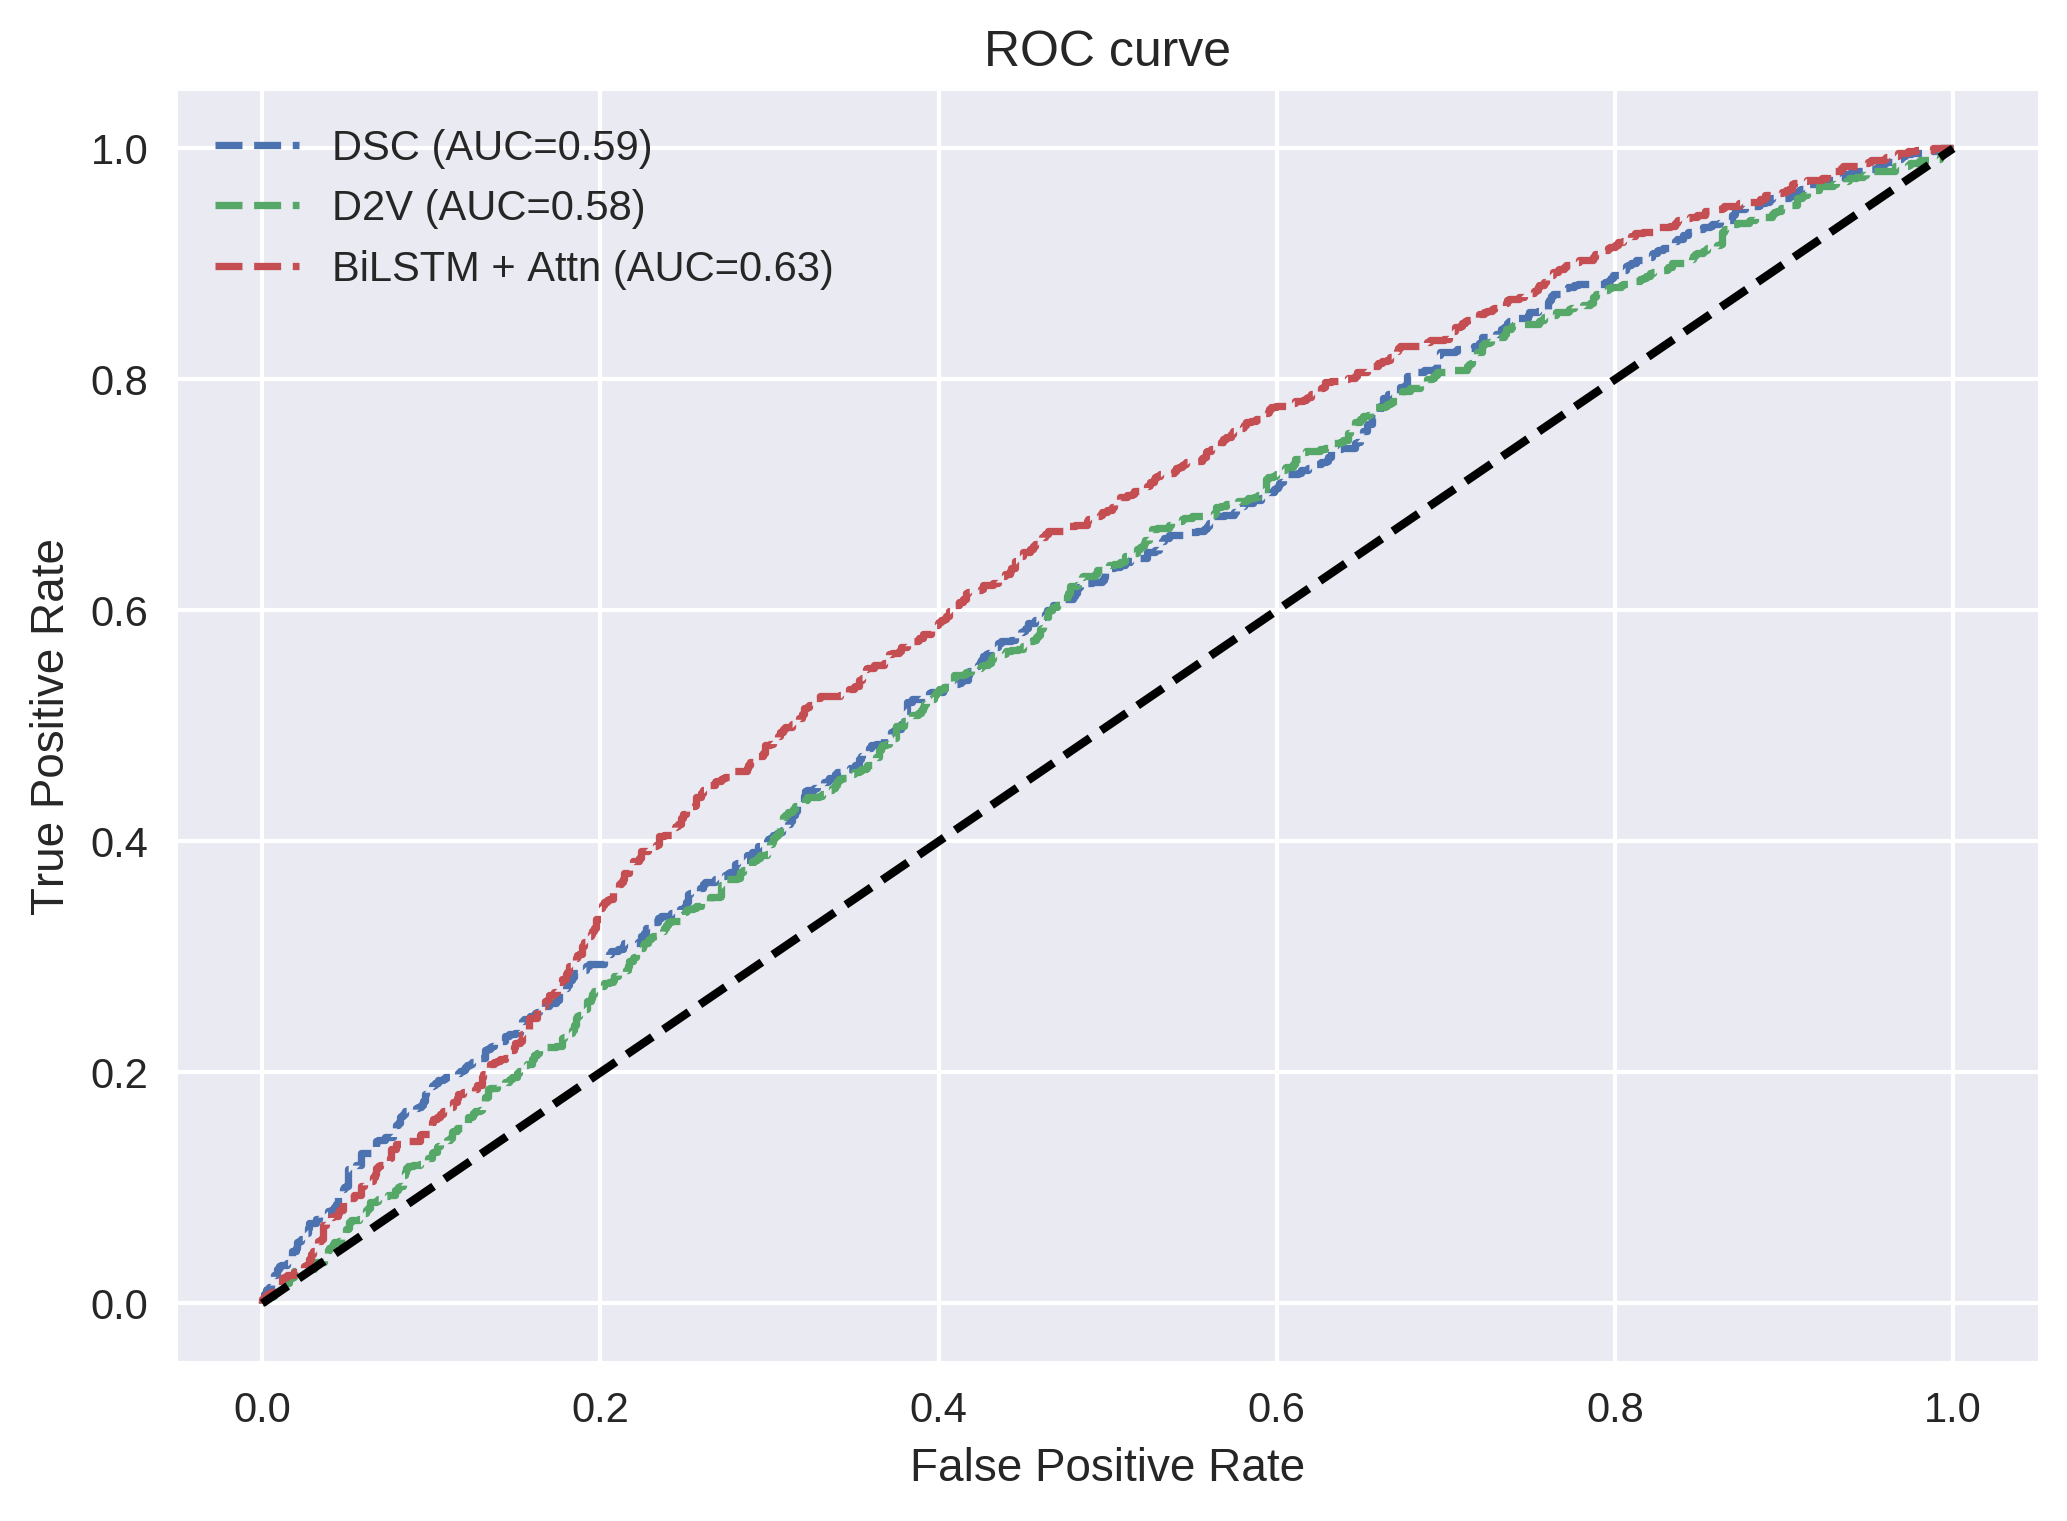
\includegraphics[width=0.7\textwidth]{../visualizations/suppa_cross_model_roc_auc_comparison.png} 
%	\caption{Example output of VOILA while filtering for LSV which only experience exon skipping and no other alternative splicing event. }
%	\label{fig:voilaexample}
%\end{figure}
\begin{savequote}[8cm]
\textlatin{Neque porro quisquam est qui dolorem ipsum quia dolor sit amet, consectetur, adipisci velit...}

There is no one who loves pain itself, who seeks after it and wants to have it, simply because it is pain...
  \qauthor{--- Cicero's \textit{de Finibus Bonorum et Malorum}}
\end{savequote}

\chapter{\label{ch:1-intro}Introduction} 

%\minitoc

"Why genes in pieces?" -- can put this citation at the top and start with related story
\section{Motivation}


\section{Contribution}




\chapter{\label{ch:2-litreview}Background} % 808 words

\minitoc

\begin{figure}[h]
	\centering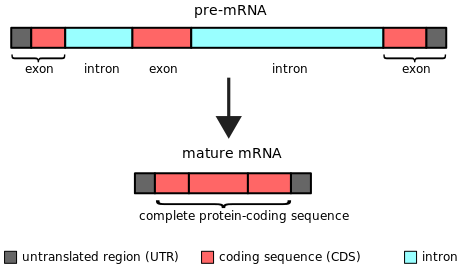
\includegraphics[width=0.9\textwidth]{../visualizations/ch2-biobackground/pre-mrna2mrna.png} 
	\caption
	{The process of splicing \cite{img:mrna}. Introns are removed from the pre-mRNA to obtain the mature mRNA only consisting of exons. Apart from coding regions, exons may also consist of non-coding untranslated regions (UTRs). Like introns, UTRs influence gene expression. 
	}
	\label{fig:pre-mrna2mrna}
\end{figure}
%TODO: do I have to explain what a gene is?
Gene expression is fundamental to all life. It is the process whereby a sequence of nucleotides is used to direct the synthesis of a functional gene product (protein, functional RNA). Gene expression occurs in two steps: during transcription, the DNA is transcribed into messenger RNA (mRNA) and during translation, the mRNA is decoded into proteins.\\
In more detail, during transcription, an initially transcribed precursor mRNA (pre-RNA) is translated into a mature RNA by a process called splicing. Splicing is based on DNA being made up of exons (predominantly coding regions), and, typically longer, introns (non-coding regions).
Only exons are contained in the mature mRNA. Introns are still contained in the initially transcribed precursor mRNA (pre-mRNA). However, they are spliced out by the spliceosome to form the mature mRNA (see Figure \ref{fig:pre-mrna2mrna}). The spliceosome is a complex molecular machine consisting of as many as 150 proteins \cite{splicing_current_perspectives}. The previous location of an intron in the transcript where two exons adjoin each other is called a splice junction or splice site.

\begin{figure}[h]
	\centering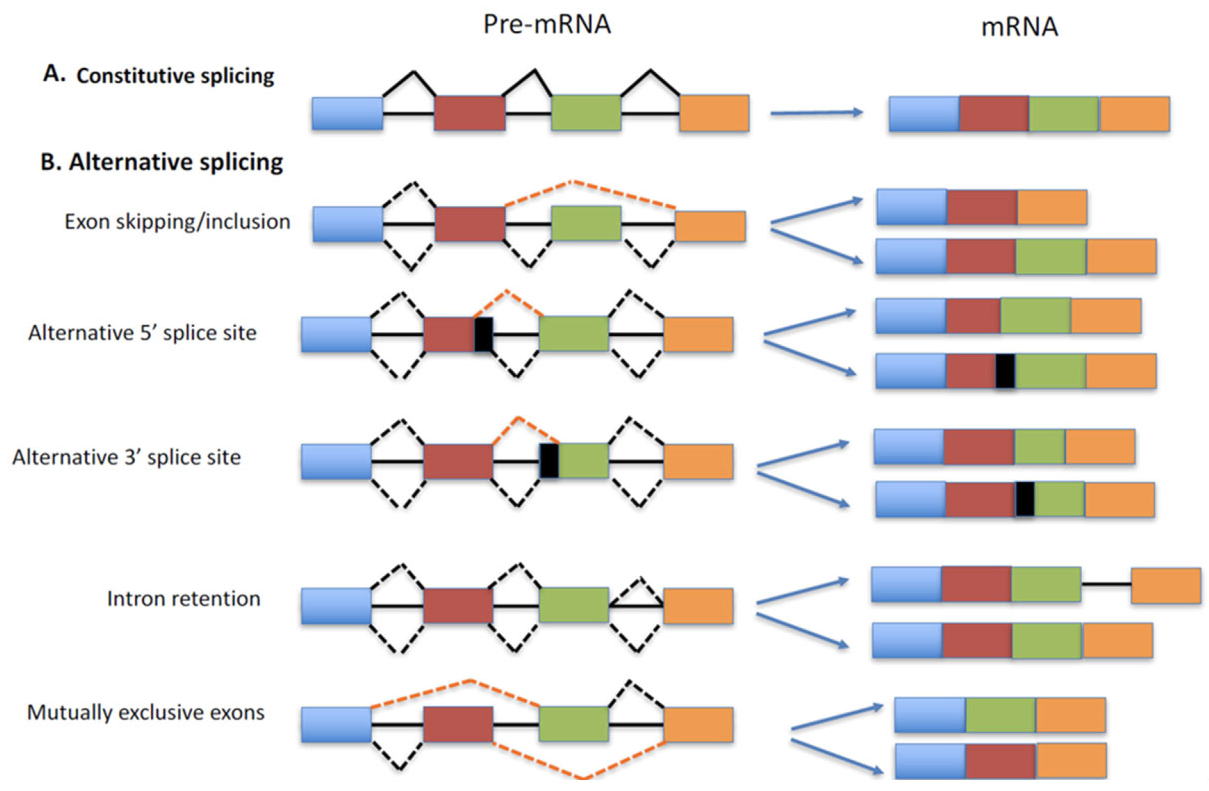
\includegraphics[width=1\textwidth]{../visualizations/ch2-biobackground/alternative_splicing_forms.png} 
	\caption
	{The most common forms of alternative splicing and the resulting different possible mature mRNAs \cite{img:altsplicingforms}.
	}
	\label{fig:altsplicingforms}
\end{figure}

Exons which are always included in the mRNA are called constitutive exons. However, 95\% of human genes with multiple exons are alternatively spliced, that is, they may only sometimes be included, or may be included with different splice sites. Alternative splicing results in the generation of multiple transcripts from a gene. The most common types of alternative splicing in higher eukaryotes are \cite{commonsplicing1}\cite{commonsplicing2}:

\begin{itemize}
\item Cassete exons are exons which are sometimes included in the mature mRNA and sometimes skipped. This is the most common form of alternative splicing in higher eukaryotes (so also humans), accounting for roughly 40\% of all AS splicing events \cite{splicing_current_perspectives}.
\item Exons with an alternative 3' or 5' splice-site. The 3' splice site or splice junction is the end of the exon towards the 3' end of the RNA strand (typically visualized as falling to the right of the sequence). The 5' splice site or splice junction is the end of the exon towards the 5' end of the RNA strand (typically visualized as falling to the left of the sequence). An alternative 3' or 5' splice-site may be located deeper inside the exon or outside the exon in a typically intronic region. Alternative 3' and 5' site splicing respectively constitute approximately 18\% and 8\% of all AS splicing events in higher eukaryotes \cite{splicing_current_perspectives}. 
\item intron retention, that is, when an intron between exons is not spliced out. It accounts for roughly 5\% of AS activity in higher eukaryotes \cite{splicing_current_perspectives}.
\end{itemize}


%TODO introduce transcripts / isforms terminology
Different forms of alternative splicing are visualized in Figure \ref{fig:altsplicingforms}. More complex forms of alternative splicing, such as mutually exclusive exons, also exist, but they are currently believed to be less common. Alternative splicing occurs in nearly all organisms that carry out pre-mRNA splicing as such as plants or animals and its frequency varies across organisms \cite{splicing_current_perspectives}. 
\subsubsection{Why does alternative splicing occur?}
Alternative splicing enables a single gene to encode multiple protein variants. This massively contributes to proteomic diversity. For instance, the roughly 20,000 human protein-coding genes are estimated to encoder over 100,000 different proteins \cite{splicing_current_perspectives}.

Alternative splicing may also speed up the rate of evolutionary adaption. Due to alternative splicing, a gene may evolve to fulfil a different functionality without first needing to evolve a separate copy of the same gene. \cite{bretschneiderphdthesis}
\subsubsection{How is alternative splicing regulated?}
Alternative splicing was discovered 40 years ago \cite{discoveryofsplicing}, but the molecular mechanisms governing it are still poorly understood. It is known that the spliceosome recognizes exon-intron boundaries based on the 5' and 3' splice sites, the branch site located in roughly the middle of the exon, and the polypyrimidine tract located upstream of the 3' splice site. However, estimates suggest that these four factors only account for half of the information required to determine splicing behaviour. The rest is likely accounted for by intronic or exonic, cis-acting sequences of the pre-mRNA which bind to trans-acting factors. These cis-acting sequences are usually 4-18 nucleotide long and classified as exonic splicing enhancers or silencers \cite{splicing_current_perspectives}.
However, the dynamic interaction between cis-acting and trans-acting factors is highly complex, new factors are still being found and thus a lot more work needs to be done if we want to fully understand alternative splicing.

%interesting papers for this:
%https://www.ncbi.nlm.nih.gov/pmc/articles/PMC4648177/
%https://onlinelibrary.wiley.com/doi/epdf/10.1002/bies.20692
%https://www.ncbi.nlm.nih.gov/pmc/articles/PMC4360811/#:~:text=Constitutive%20splicing%20is%20the%20process,various%20forms%20of%20mature%20mRNA.
\subsubsection{What happens when splicing is misregulated?}
Since alternative splicing is such a fundamental mechanism, its correct execution is crucial. Defects in splicing are typically caused by genomic sequence variations leading to misregulation of the splicing process. An estimated 9\%-30\% of Mendelian disorders may act through disruption of splicing \cite{comparison}
Splice variants have also been shown to be biomarkers for multiple types of cancers \cite{cancer} \cite{splicingcausescancer}. As a result, alternative splicing has also been suggested as a biomarker and potential target for drug discovery \cite{drugdiscoverysplicing}. \\

%TODO: more about disease and splicing
% https://www.sciencedirect.com/science/article/pii/S001457930500253X -- 50% mutation disease from splicing
% big nature splicing in disease paper: https://www.nature.com/articles/nrg2164?cacheBust=1508215213365

%TODO: add these caner quoations
% Alternative splicing of fibroblast growth factor receptor 2 (FGF-R2) in human prostate cancer, -1997 meh
%Modification of alternative splicing pathways as a potential approach to chemotherapy,
% Discovery of novel splice forms and functional analysis of cancer-specific alternative splicing in human expressed sequences - done
% Computational analysis and experimental validation of tumor-associated alternative RNA splicing in human cancer - 
% many human genetic diseases: Pre-mRNA splicing and human disease
\subsubsection{Importance of understanding splicing}
Thus, there is great interest in better understanding the mechanisms underpinning alternative splicing. Due to rapid advances in RNA sequencing technologies, it is now possible to sequence the genome of a patient within a day. However, the genomic variants (compared to a reference genome) observed in patients are often variants of unknown significance. \cite{bretschneiderphdthesis} That is, it is unknown whether these variants are pathogenic or benign. An improved understanding of alternative splicing may improve the classification of genomic variants and help with the diagnosis of patients, especially those with rare genomic diseases.

\chapter{\label{ch:3-relatedwork}Related work} % 920 words

Splicing codes are computational models that attempt to predict splicing behaviour based on putative regulatory features (such as sequence motifs).
They were first introduced in the seminal papers by \cite{barash2010a}\cite{barash2010b}. Their introduction was motivated by the recognition that splicing is highly condition-specific and regulated by the complex interaction of many factors in such a way that it is only feasible to model this behaviour computationally.\\
\cite{barash2010a} focus on cassette exons and attempt to predict the change in splicing behaviour for a given exon between different tissues. They popularized the use of the quantitative measure PSI (sometimes denoted $\Psi$) to describe splicing behaviour:
PSI is defined as the proportion of transcripts out of all transcripts that contain a given exon \cite{psi}. In other words, given a random transcript, PSI denotes the probability of a particular exon being included or excluded.\\
%Similarly, $\Psi_5$ is defined as the number of transcripts containing a particular alternative 3' splice site for a fixed 5' splice site. $\Psi_3$ is defined analogously as the number of transcripts containing a particular alternative 5' splice site for a fixed 3' splice site. $\Psi_5$ and $\Psi_3$ are particularly interesting to model the competition between different alternative splice sites.
To quantify the change of splicing behaviour between conditions, these models predict the corresponding $\Delta$PSI. They were able to find novel regulators of key genes associated with diseases and to predict how genetic variants will affect splicing \cite{splicingcodegood1} \cite{splicingcodegood2}. Input to the model are over 1000 known and unknown motifs and higher-level features (such as exon/intron lengths and phylogenetic conversation scores) selected partially from previous studies and partially from de novo searches.


Improving upon these first models, the `second generation' of splicing codes used several common and uncommon machine learning algorithms such as multinomial logistic regression, support vector machines (SVM) and Bayesian Neural Networks (BNN) to predict changes in alternative splicing behaviour. \cite{bnnsplicing} Among these, BNNs were able to outperform the other methods when evaluated on a microarray dataset based on mouse data. In contrast to models from the first generation, BNNs based models only took in sequence information and very high-level features like tissue type which meant that the model were automatically able to learn relevant motifs from the data.


However, BNNs often rely on expensive sampling methods like Markov Chain Monte Carlo (MCMC) to be able to sample models from a posterior distribution. It can be challenging to scale these methods to larger datasets and a large number of hidden variables.
As a result, the `third generation' of splicing codes relies on Deep Learning models which can effectively make use of the large amount of data available with the advent of high-throughput RNA-sequencing technologies. First forays into using Deep Learning-based models were made by \cite{leung2014}. Using a Deep Neural Network (DNN) with an autoencoder, they were able to improve upon the results achieved by BNN models. Albeit \cite{leung2014} initially used a different dataset and a different task formulation than \cite{bnnsplicing}, \cite{jha} were able to show that these improvements also lasted when directly comparing the models on the same dataset using the same task formulation. Furthermore, \cite{jha} developed a framework for integrating further experimental data, like data from CLIP-seq based measurements of in vivo splice factors bindings, into the model developed by \cite{leung2014}. Adding these additional features improved the explained variance in splicing behaviour between tissues, as measured by the $R^2$ score, by roughly further 5\% to an overall average value of 43.4\%.
Taking inspiration from advances in Natural Language Processing, \cite{d2vsplicing} developed splicing codes based on the automated feature learning approach from word2vec and doc2vec. Developing two models, one based on doc2vec and a simple MLP, and one based on word2vec and the all-convolutional Inception architecture known from Computer Vision \cite{inception}, they were able to achieve an average $R^2$ score of 69.2\% significantly improving upon the predictive power of previous models.


In contrast to these splicing codes which predict the (differential) inclusion frequency of an exon, a parallel strand of research focuses on splicing codes for distinguishing between constitutive and alternatively spliced exons. For the first task the dataset the models are trained on only consists of alternatively spliced cassette exons and the models have to find features that are predictive of the exact inclusion rate of an exon.\\
For the second task, the dataset consists of alternatively spliced as well as constitutive exons and the models have to find features predictive for distinguishing between constitutive and alternatively spliced exons.
While there is a large overlap between these features, there are also differences.
For predicting the inclusion level of an exon, features from the cassette exon and the surrounding exons have shown been reported to be required \cite{splicingcodegood1}. For predicting whether an exon is constitutive or not, features around the cassette exon itself have been shown to be the most critical \cite{featurearoundexonjunc}. 
%[possibly talk more about features used by dsc and what constitutive exons could use]

\cite{buschhertel} used 262 features extracted from an exon and its two flanking introns to train an SVM-based splicing code for distinguishing between constitutive exons, cassette exons and exons with an alternative 5' or 3' splice site. The dataset used to train the model was based on roughly 4 million ESTs and known isoforms, as well as the alternative events, track (Alt Events) of the UCSU Genome Browser.\\
Their model achieved very impressive results with an AUC of roughly 0.94 when differentiating between rarely included and constitutive exons, but performance decreases to roughly 0.60 when distinguishing between frequently included and constitutive exons. \cite{dsc} improved upon this work by using a Deep Learning model which was automatically able to learn relevant features from the raw sequence. Their model was based on a combination of convolutional blocks for feature extraction as well as an MLP for classification based on the extracted features. Training on a similar EST-based dataset, their model is significantly more robust when distinguishing between highly included cassette exons and constitutive exons with the AUC only dropping to ~0.85. When distinguishing between rarely included cassette and constitutive exons, it was still able to achieve an impressive AUC of ~0.92.

\chapter{\label{ch:4-methods}Methods}

%TODO: short name for attention model
% TODO: fix attention formulas
%TODO: citations not working

This chapter introduces the primary data sources, describes how these were used to obtain the training datasets, and presents the used models. It also gives implementation details regarding processing steps, model implementation, and model training.
In this work, we focus on the splicing prediction of cassette exons. Previous work indicates that advances in predicting one type of alternative splicing behaviour via Machine Learning methods also translates to advances in prediction for other types. Therefore, a practical choice is to only focus on one splicing type as this reduces the number of experiments and needed training time by two to three factors. As noted, cassette exons are the most common form of alternative splicing in higher eukaryotes. Thus, for reasons of practicality we choose cassette exons as the type of alternative splicing, we will focus on.
\section{Datasets}\label{sec:datasets}
Three primary sources for genomic data were used in this study: the Human Exon splicing events (HEXEvent) database \cite{hexevent}, data from the Genotype-Tissue Expression (GTEx) project \cite{gtex} and data from the Human Induced Pluripotent Stem Cell Initiative (HipSci) \cite{hipsci}. Except for the HEXEvent database, none of these primary sources directly report the PSI values of exons or junctions. The processing done to estimate the PSI value-based from the primary sources is described in section [estimating PSI]. All of the data sources required further processing (e.g. extraction of corresponding nucleotide sequences) to obtain the final samples which are the input for the models. These further processing steps are described in section [final sample processing]
The HEXEvent database contains genome-wide exon data sets of human internal exons which can be filtered for selected splicing events (e.g. constitutive or cassette exons) via an online user interface. It was compiled based on known mRNA variants as defined by the UCSC Genome Browser (newest version is hg38) as well as their associated available expressed sequence tag (EST) information.
It was chosen as a data source for direct comparability with the baseline paper \cite{dsc}.
TODO critizie est data
%TODO criticize EST data
these are sequence reads datasets based on which I will estimate the PSI values
\subsection{GTEx} \label{subsec:gtex}
The Genotype-Tissue Expression (GTEx) project provides the most comprehensive database for tissue-specific gene expression and regulation available to-date. It contains over 17000 samples from nearly 1000 human donors. Each sample was taken from up to 54 different tissue sites. The sequencing samples were obtained using mainly molecular assay-based techniques like Whole Genome Genotyping (WGS), Whole Exome Sequencing (WES) and RNA-Seq.
Processed data which can not be used to identify the donors is publicly available on the GTEx portal. To access raw data (e.g. raw RNA-seq reads) and meta-information about the samples one is required to undergo a data access request. It is intended that data access is requested by PIs or leader of research groups for their whole lab. Approval of a data access request usually takes upwards of 3 months. The co-collaborators Prof. Wilfred Haerty and Prof. Elizabeth Tunbridge have access to the protected part of the GTEx data. However, the scope of projects for which they were granted access does not include this thesis and changing the scope would require undergoing the data access process again. For this reason, we only use the publicly available part of the GTEx data, in particular the files containing information about exon-exon junction reads.
%using gtex:
%'We strongly recommend the use of TPM (Transcripts Per Million), because is normalized for gene length first, and then for sequencing depth. This allows a direct comparison between samples' https://github.com/comprna/SUPPA/wiki/SUPPA2-tutorial
%good site: https://www.ncbi.nlm.nih.gov/projects/gap/cgi-bin/study.cgi?study_id=phs000424.v8.p2
\subsection{HipSci} \label{subsec:hipsci}

\begin{figure}
	\centering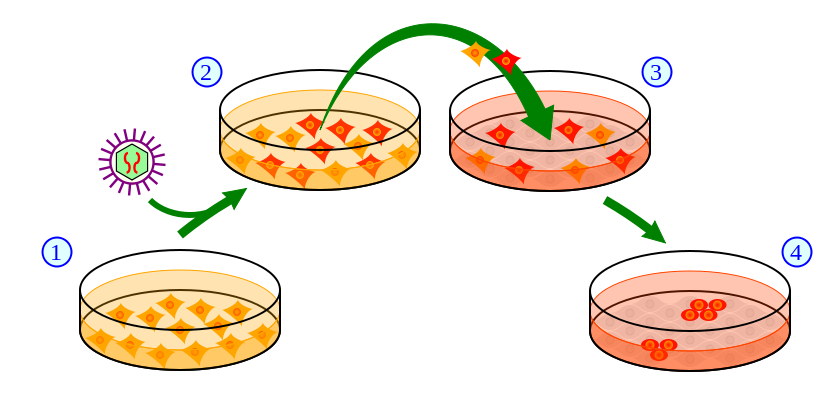
\includegraphics[width=0.7\textwidth]{../visualizations/ipscprocess.png} 
	\caption[test.]{
	(1) Cell culture of donor cells is grown. (2) Transduce the genes associated with reprogramming into the cells via viral vectors. (3) Isolate the cells expressing the transduced genes (in red) and culture them according to embryonic stem cell culture. (4) A small subset of the transfected cells become iPSC cells. Graphic and description adapted from \cite{ipscprocess}.
}
	\label{fig:ipscprocess}
\end{figure}

The Human Induced Pluripotent Stem Cell Initiative (HipSci) is a large, mostly freely-available repository of human induced pluripotent stem cell (iPSC) lines. iPSC cells are mature cells which have been reprogrammed to again become pluripotent (undetermined). Figure \ref{fig:ipscprocess} shows how iPSC cells are obtained. As iPSC cell lines are not directly obtained from human donors, but rather from building a cell culture based on some initial donor cells, the HipSci dataset does not suffer from the data privacy issues which prevented access to the raw RNA-seq reads as in the GTEx data.


Over 300 cell lines from over 300 donors along with their RNA-seq reads are publicly available from the HIPSCI portal. From these we selected two groups of roughly 20 biological replicates each:
Neuron cell lines: One group of biological replicates were taken from undifferentiated iPSC cells from donors from which at least two cell lines are available. This allows testing how well the learned features of the model translate when applied to another library of the same tissue type from the same individual.
iPSC cell lines: One group of 25 biological replicates were taken from iPSC cells differentiated to sensory neuron cells. This allows testing how well the learned features of the model translate when applied to another library of different tissue.
iPSC background probably here:
some section about iPSC cells as relevant later on -- might skip all of this:
The Nobel Prize in Physiology or Medicine of 2012 was awarded to Shinya Yamanaka and Sir John Gurdon "for the discovery that mature cells can be reprogrammed to become pluripotent". Pluripotent cells are cells which can differentiate into other cell types.
process: take cell samples, then grow cell culture, make them pluripotent and use the pluripotent cells to differentiate into other ones
\section{Data processing}\label{sec:dataprocessing}
\subsection{Estimating PSI} \label{subsec:psiestimation}
An often used quantitative measure is per cent spliced-in (PSI or $\Psi$).
$\Psi$ is defined as the proportion of transcripts out of all transcripts that contain a given exon \cite{psi}. In other words, given a random transcript, it denotes the probability of a particular exon being included or excluded.
Similarly, $\Psi_5$ is defined as the number of transcripts containing a particular alternative 3' splice site for a fixed 5' splice site. $\Psi_3$ is defined analogously as the number of transcripts containing a particular alternative 5' splice site for a fixed 3' splice site. $\Psi_5$ and $\Psi_3$ are particularly interesting to model the competition between different alternative splice sites.
High-throughput sequencing of cDNA fragments (RNA-seq; Lister et al., 2008) has become a popular tool to investigate RNA expression and post-transcriptional regulation. Sequencing of the transcriptome reveals tens of thousands of transcripts expressed simultaneously (Mortazavi et al., 2008). Despite providing a deep and genome-wide view on post-transcriptional processing, current technologies cannot reveal transcripts in full-length due to limitations in read length. %TODO: fix citations here [https://www.researchgate.net/publication/282645615_Alternative_Splicing_Signatures_in_RNA-seq_Data_Percent_Spliced_in_PSI/link/59e8404b458515c3630fe4e3/download]
High-throughput sequencing methods are a potent tool to investigate RNA expression and post-transcriptional regulation. However, due to limited coverage, short read length, and experimental biases they are not able to provide a full view of post-transcriptional processing so far.
However, due to limitations in read length, they are not able to provide a full view of post-transcriptional processing so far.
%[majiq + berlin, https://elifesciences.org/articles/11752#abstract]
'Despite constant technological advancement, the combination of limited coverage depth, experimental biases, and reads spanning only a small fraction of the variable parts of transcripts has left accurate mapping of transcriptome variations an open challenge (Alamancos et al., 2014).'
\subsubsection{Naive PSI estimation}\label{subsubsec:naivepsi}

Let \#IR be the number of reads giving evidence for a particular exon being included. Let \#ER be the numbers of reads giving evidence for a particular exon being excluded. A PSI value of 100\% indicates a constitutive exon which is always included, a score below 100\% includes an alternatively spliced exon. Figure MISO graphic] or ![berlin graphic, should then mention that it shows the full pipeline from going from reads to PSI] shows examples of possible reads counted in pos and neg. PSI can then be estimated as:
$$PSI = \frac{\#IR}{(\#IR+\#ER)}$$
The advantage of this estimate lies in its flexibility. It is very to implement and not very error-prone. It is independent of library size. It can easily be adapted to estimate the PSI of a junction by redefining \#IR and \#ER to count the inclusion and exclusion read for that junction.
'deceptively simple'?
%TODO: [Using Naive PSI with GTEx data (or similar)]
However, this estimate has various issues. [todo formatting -- itemize]
\begin{enumerate}
	\item It doesn't account for uncertainty in the estimate. A rarely expressed gene may only experience a few reads of a particular exon leading to a very uncertain estimate. For instance, if we observe 1 IR and 1 ER for exon E1: $PSI_E1 = \frac{1}{2} = 50\%$. Compare this to E2 where we observed 15 inclusion and 15 exclusion reads: $PSI_E2 = \frac{15}{30} = 50\%$.\\
	The estimate of $PSI_E2$ is likely to be more accurate, but this information is not contained in the estimate. Concretely, these two samples would be treated as equally important by the network even though perhaps they shouldn't.
	A further processing step to only count exons who experienced at least threshold number of reads only alleviates this problem. One would need to account for the expressiveness of each gene because 10 reads in a lowly expressed gene may be as significant as 20 reads in a highly expressed gene. There are several measures for the expressiveness of a gene: Reads Per Kilobase Million (RPKM), Fragments Per Kilobase Million (FPKM) and Transcripts Per Kilobase Million (TPM) and although TPM is the most common one, it is not obvious that it is the best choice in this scenario.
	% https://www.rna-seqblog.com/rpkm-fpkm-and-tpm-clearly-explained/
	
	%TODO: could add that even then reads across a gene aren't normally distributed
	
	Assuming that one obtains a read count normalized by the gene expressiveness for each exon, there is not a principled way to choose the cutoff threshold. The choice between a threshold which e.g. filters 5\% or 20\% of the samples is a trade-off between data quality and training samples.
	\item Reads which align purely to the flanking constitutive exons are ignored. While these could have occurred in either isoform, they provide latent evidence for whether the cassette exon was included or not. In isoforms where it occurred, the total length of the isoform is longer which means the reads are distributed over a larger area. This leads to a comparatively reduced proportion of reads across the flanking exons when the exon was included and vice versa. The estimate neglects to take this information into account.
%	This estimate ignores reads that align to the bodies of the flanking constitutive exons, which could have derived from either isoform. Nevertheless, these constitutive reads contain latent information about the splicing of the alternative exon, as higher expression of the exclusion isoform will generally increase the density of reads in the flanking exons relative to the alternative exon, and lower expression of the exclusion isoform will decrease this ratio of densities.
%	[MISO]
%	this is the reason why I wanted access to raw RNA-seq reads
	\item Related to 1), typically multiple samples or biological replicates of a given experiment are available. It is desirable that reads across multiple samples can be integrated to give a more well-adjusted estimate. How to best achieve this is not obvious. Read depths between multiple libraries may vary and this should be accounted for. [possible other issues here and then make this another itemization]
	\item IR and ER must be normalized for exon length to obtain meaningful results. For a long exon, the majority of reads will be IR because they can be located over a much larger area than the ER who must overlap with the 0-length feature of the splicing junction. This can be accounted for by normalizing for the possible number of start positions for each read population:
	$$\#IR_norm = \frac{\#IR}{(exon length + read length -1)}$$
	$$\#ER_norm = \frac{\#ER}{(read length - 1)}$$
	Note that this assumes that reads are uniformly distributed across a transcript isoform. It is well-known that RNA-seq reads are biased .... [get paper from Liz/Wilfred]
	
	%	thought: this normalization doesn't obviously seem correct to me on second thought. an ER can be found at two junctions, so that would double the number of possible read starts
	%	IR can only start from position 0 to exon.length-read.length of the exon can't they?
	%	won't do anything about this, but will want to use weaker claim
	%	I think you can't really do normalization for junction counting
\end{enumerate}



%hopefully was able to demonstrate that this estimate is problematic and may easily be unreliable.
Due to these issues relating to the uncertainty, to not making use of all of the available evidence and to integrating reads across multiple samples, this estimate is problematic.
\subsubsection{How I implemented PSI estimation}
%TODO write this section

1) Only take reads from genes across a certain TPM into account (because random spurios reads from low TPM genes could have an outsized effect on the estimation). Say that you weight reads according to the respective TPM. Show TPM distribution and say what TPM threshold you use.\\
2) Say how there is nothing you can do, due to only having access to the junction reads themselves. \\
3) Unclear how to best do this and skipped for now. However, basing estimatin based on the sample with the maximum total amount of reads. \\
4) Say that you estimate read length to be 150 and do this. \\
 TODO: mention junction datasets
% potentially even more details; eg how you use this heuristic of checking the 10 samples past the current one
% todo add details such as exact name of individuals used and number of reads
Several approaches have been developed which try to address these issues in estimating PSI. However, many of these focus purely on the differential splicing changes between conditions (in the form of delta PSI) and don't directly report the PSI in a given condition which is what we are initially interested in. Of the methods directly reporting PSI, we chose the two fast methods SUPPA and MAJIQ. SUPPA and MAJIQ represent two different approaches to PSI estimation: SUPPA is primarily based on quantification of transcripts, while MAJIQ is based on building up a splicing graph.


%isoform-based vs count-based methods
%	count-based methods = exon based and event-based methods
\subsubsection{SUPPA}\label{subsubsec:suppa}
SUPPA2 \cite{suppa2} estimates the PSI value for each alternative splicing event based on transcript abundances. It operates in 2 steps for quantifying the PSI of an alternative splicing event:
1) Given an input annotation file in GTF format, it generates the transcript isoforms which count as IR or ER for a given alternative splicing event.
2) Given the information which transcript count as IR or ER from 1) and how frequently each transcript occurs, it estimates the PSI value via $$PSI = TPM_IR / TPM_IR + TPM_ER$$. SUPPA2 can integrate the TPM values from multiple samples.
%because it is so naive is probably the reason why it performs so badly
%!perhaps add steps 1/2/3 to this graphic?
\textbf{Using SUPPA2:}
SUPPA2 requires a GTF annotation file and a file quantifying the abundance of each transcript. A GENCODE version 34 annotation file obtained from Ensembl was used as an annotation file. Salmon was used for quantifying the relative abundance of each transcript in TPM. Salmon's [cite] quantification is based on the raw RNA-seq reads in FASTQ format, takes into account experimental attributes and correct for biases commonly observed in RNA-seq data. After extracting the TPM values provided by Salmon into the format required by SUPPA (a tsv-file with one column for the transcript id and one column for the TPM value), SUPPA2 estimates the PSI for each alternative splicing event.
The latest version of SUPPA available as of July 2020 was used (SUPPA v2.3). 
%[https://github.com/comprna/SUPPA/releases/tag/v2.3 if I feel like it]
\subsubsection{MAJIQ}\label{subsubsec:majiq}
Modeling Alternative Junction Inclusion Quantification (MAJIQ) builds up a splice graph \cite{majiq2} which contains exon as vertices and junctions as edges. An edge is added between two vertices if a transcript isoform is found in which they share a junction (that is if the exons are neighbours and everything between them has been spliced out).
Constitutive exons are vertices with two incoming edges.
Vertices which have more than 3 incoming edges are denoted as local splicing variations (LSV). Due to this problem formulation, MAJIQ can model more complex splicing variations than skipped exons, alternative 3' splice sites, and alternative 5' splice sites. Importantly, apart from estimating $\delta$ PSI between different conditions, MAJIQ is also able to directly estimate PSI for a given condition. The estimation is done using a combination of read rate modelling, Bayesian PSI modelling and bootstrapping.\\
%TODO !graphic -- remove this grey line, perhaps point out splicing variants in graphic
\textbf{Using MAJIQ:} MAJIQ requires sequence files in bam format (along with the index in bai format) and an annotation DB in gff3 format. The bam format is a format for aligned RNA-seq reads. 
%todo [what does index file do?]
To this end, the raw reads from each sample were uploaded to the bioinformatics data processing platform Galaxy \cite{galaxy} from the European Nucleotide Archive (ENA). For each sample, the raw reads in FASTQ format were then mapped to the RNA using STAR \cite{star}. STAR produces the required bam and bai format files as output.

The required gff3 file used is human GRCh38 release 13.
MAJIQ use then proceeds in three stages. First MAJIQ Builder takes a configuration file, the gff3 annotation and the bam and bai files of all samples as input and builds up the splicing graph. At this stage, MAJIQ also identifies constitutive exons and optionally dumps them to a file. This option was used.
Secondly, MAJIQ PSI estimates the PSI of the LSV candidates obtained through MAJIQ Builder. MAJIQ PSI improves the accuracy of its PSI estimate by integrating evidence across multiple samples.
Finally, the obtained LSVs can be visualized using VOILA. VOILA also allows filtering of LSV according to type. See Figure \ref{fig:voilaexample} for an example output of VOILA. For this study, only LSV which denoted exon skipping were used. The filtered LSV along with the constitutive exons obtained from MAJIQ Builder were then used for processing as described in Section [section where I describe sequence extraction, mirroring for negative-strand etc]
The latest version of MAJIQ available as of July 2020 was used (MAJIQ v2.0).


\begin{figure}
	\centering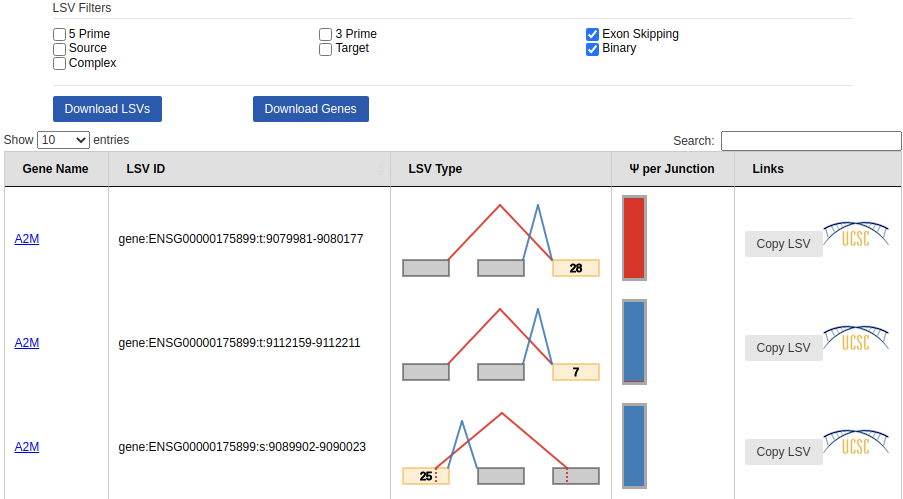
\includegraphics[width=0.7\textwidth]{../visualizations/voila_example.png} 
	\caption[Four-chamber illustration of the human heart.]{Example output of VOILA while filtering for LSV which only experience exon skipping and no other alternative splicing event. }
	\label{fig:voilaexample}
\end{figure}

%TODO: what does [] after caption do?
%TODO: look into hyperref etc

The naive way of estimating PSI was applied to the GTEx dataset as we had no access to raw RNA-seq reads and couldn't apply SUPPA nor MAJIQ. SUPPA and MAJIQ were applied to the data from the HipSci repository.
\subsection{Final sample processing} \cite{subsec:finalsampleprocessing}

\begin{figure}
	\centering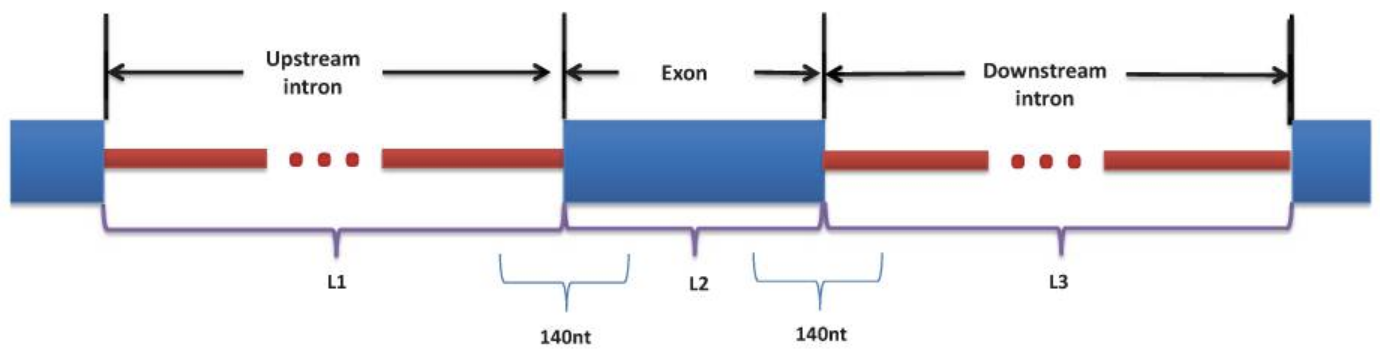
\includegraphics[width=0.7\textwidth]{../visualizations/input_schematic.png} 
	\caption[bla.]{The input to our models are the 140 nucleotide region extracted around the exon start and exon end, as well as the normalized length of the exon and its flanking introns. }
	\label{fig:inputschematic}
\end{figure}

Using the output of the previous preprocessing steps, now either exon-centric or intron-centric samples are created. Exon-centric samples are created when the task of the network is to classify an exon as constitutive or not. Intron-centric samples are created when the task of the network is to classify whether a junction is constitutive or not.
At this point, the datasets have been preprocessed that each sample at least contains the following:
chromosome and strand information of the to-be-classified exon or junction
start and end coordinates of the exon or junction within a chromosome,
the lengths of neighbouring introns or exons.
Using the chromosome information and the start and end coordinates, a 140 nucleotide window around the start and end coordinates are extracted (see Figure \ref{fig:inputschematic}). Furthermore, if an exon or junction is taken from a negative strand, the extracted start and end windows are switched, the order of the nucleotides within the start and end windows are reversed and each extracted nucleotides is converted to its reverse complement. This way the models don't have to learn different features for exons or junctions on the + and - strand.
Samples from the chromosomes X, Y and M were excluded as these are known to show special splicing behaviour. [citation needed]
%TODO: what exact formulation did will / liz use here?
The extracted nucleotides were one-hot encoded as four dimensional vectors. Specifically, adenine 'A' was encoded as [1 0 0 0], cytosine 'C' as [0 1 0 0], guanine 'G' as [0 0 1 0] and thymine 'T' as [0 0 0 1]. Thus each 140 nucleotide long window was converted into an 140x4 matrix containing one-hot encodings.
It is commonplace that repetitive sequences are soft-masked as lower case letters in the reference genome. As this has no bearing on alternative splicing, this information was ignored during one-hot encoded.
In addition to sequence information, the lengths of neighbouring introns or exons, as well as the length of the exon itself, are given as input to the models. Several studies have shown that exon and intron lengths can influence splice-site recognition. [15,34] In addition, previous studies have shown that including the length information dramatically model performance. [DSC] Introns are on average one to two orders of magnitudes larger than exons and their relative standard deviation is three times as large as that of exons. To avoid giving features to the network whose magnitude might differ by several orders of magnitude, the intron and exon lengths features were respectively normalized through the mean length and standard deviations of internal exon and introns in the human genome \cite{exonintronlens}. For brevity, these lengths are often referred to as the length features.
%TODO [maybe but probably not: exon_mean, exon_std, intron_mean, intron_std = 145.42, 198.0, 5340., 17000.]
Some of the datasets had a class imbalance issue between constitutive and alternatively spliced samples. For instance, the HexEvent dataset contains roughly times three as many constitutive as alternatively spliced samples. This leads to the issues with models getting stuck in local minima where they just predict the majority class. This was alleviated by including each alternatively spliced sample multiple times until the classes were balanced.
A single sample input to the model contains two 140x4 one-hot encoded matrixes and three normalized length values. The associated ground truth with each sample is the scalar 1 if the respective exon or junction is constitutive, and 0 if not.
\subsection{Dataset statistics} \cite{subsec:datasetstatistics}

%TODO: Table [in overleaf atm] shows the absolutes number of obtained training samples for all datasets which were used.
further analysis postponed until I ran experiments again and decided for which datasets I will show results 

hexevent:
Total number of exons: 50918
Number of low PSI exons: 39128
Number of high PSI exons: 4952
Number of cons exons: 6838
gtex exon brain
Number of generated training samples: 32682
Number of low PSI exons: 15872
Number of high PSI exons: 7961
Number of cons exons: 8849
gtex exon cerebellum
Number of generated training samples: 39874
Number of low PSI exons: 19355
Number of high PSI exons: 6791
Number of cons exons: 13728
gtex exon heart
Number of generated training samples: 20806
Number of low PSI exons: 9569
Number of high PSI exons: 5216
Number of cons exons: 6021
gtex junction brain
Number of generated training samples: 127908
Number of low PSI exons: 58560
Number of high PSI exons: 14538
Number of cons exons: 54810
gtex junction heart
Number of generated training samples: 81659
Number of low PSI exons: 36354
Number of high PSI exons: 9389
Number of cons exons: 35916
gtex junction cerebellum
Number of generated training samples: 161310
Number of low PSI exons: 74139
Number of high PSI exons: 13151
Number of cons exons: 74020
gtex reconstruction junc (brain)
Number of skipped non-DSC junctions: 71868
Number of low PSI junctions: 23943
Number of high PSI junctions: 7281
Number of cons junctions: 25977
Total number of junctions: 57201
gtex reconstruction exon (brain)
Number of low PSI exons: 3458
Number of high PSI exons: 1989
Number of cons exons: 23505
Total number of exons: 28952
hipsci majiq junc (neuron)
total: 90627
Number of cons junctions: 48163
Number of alt juncs: 42464 (from 21232 exons)
Number of low PSI exons: 22834
Number of high PSI exons: 19630
hipsci majiq exon (neuron)
total: 44746
Number of cons exon: 26394
Number of alt exons: 18352
Number of low PSI exons: 8201
Number of high PSI exons: 10151
hipsci suppa exon (neuron)
Number of samples: 17863
Number of low PSI exons: 9828
Number of high PSI exons: 311
Number of cons exons: 7724
hipsci majiq exon (iPSC)
total: 48489
Number of cons exon: 27371
Number of generated training samples: 21118
Number of low PSI exons: 9299
Number of high PSI exons: 11819
some analysis of the numbers, e.g. junction datasets way larger
probably won't include reconexon/junction dataset

\begin{figure}
	\centering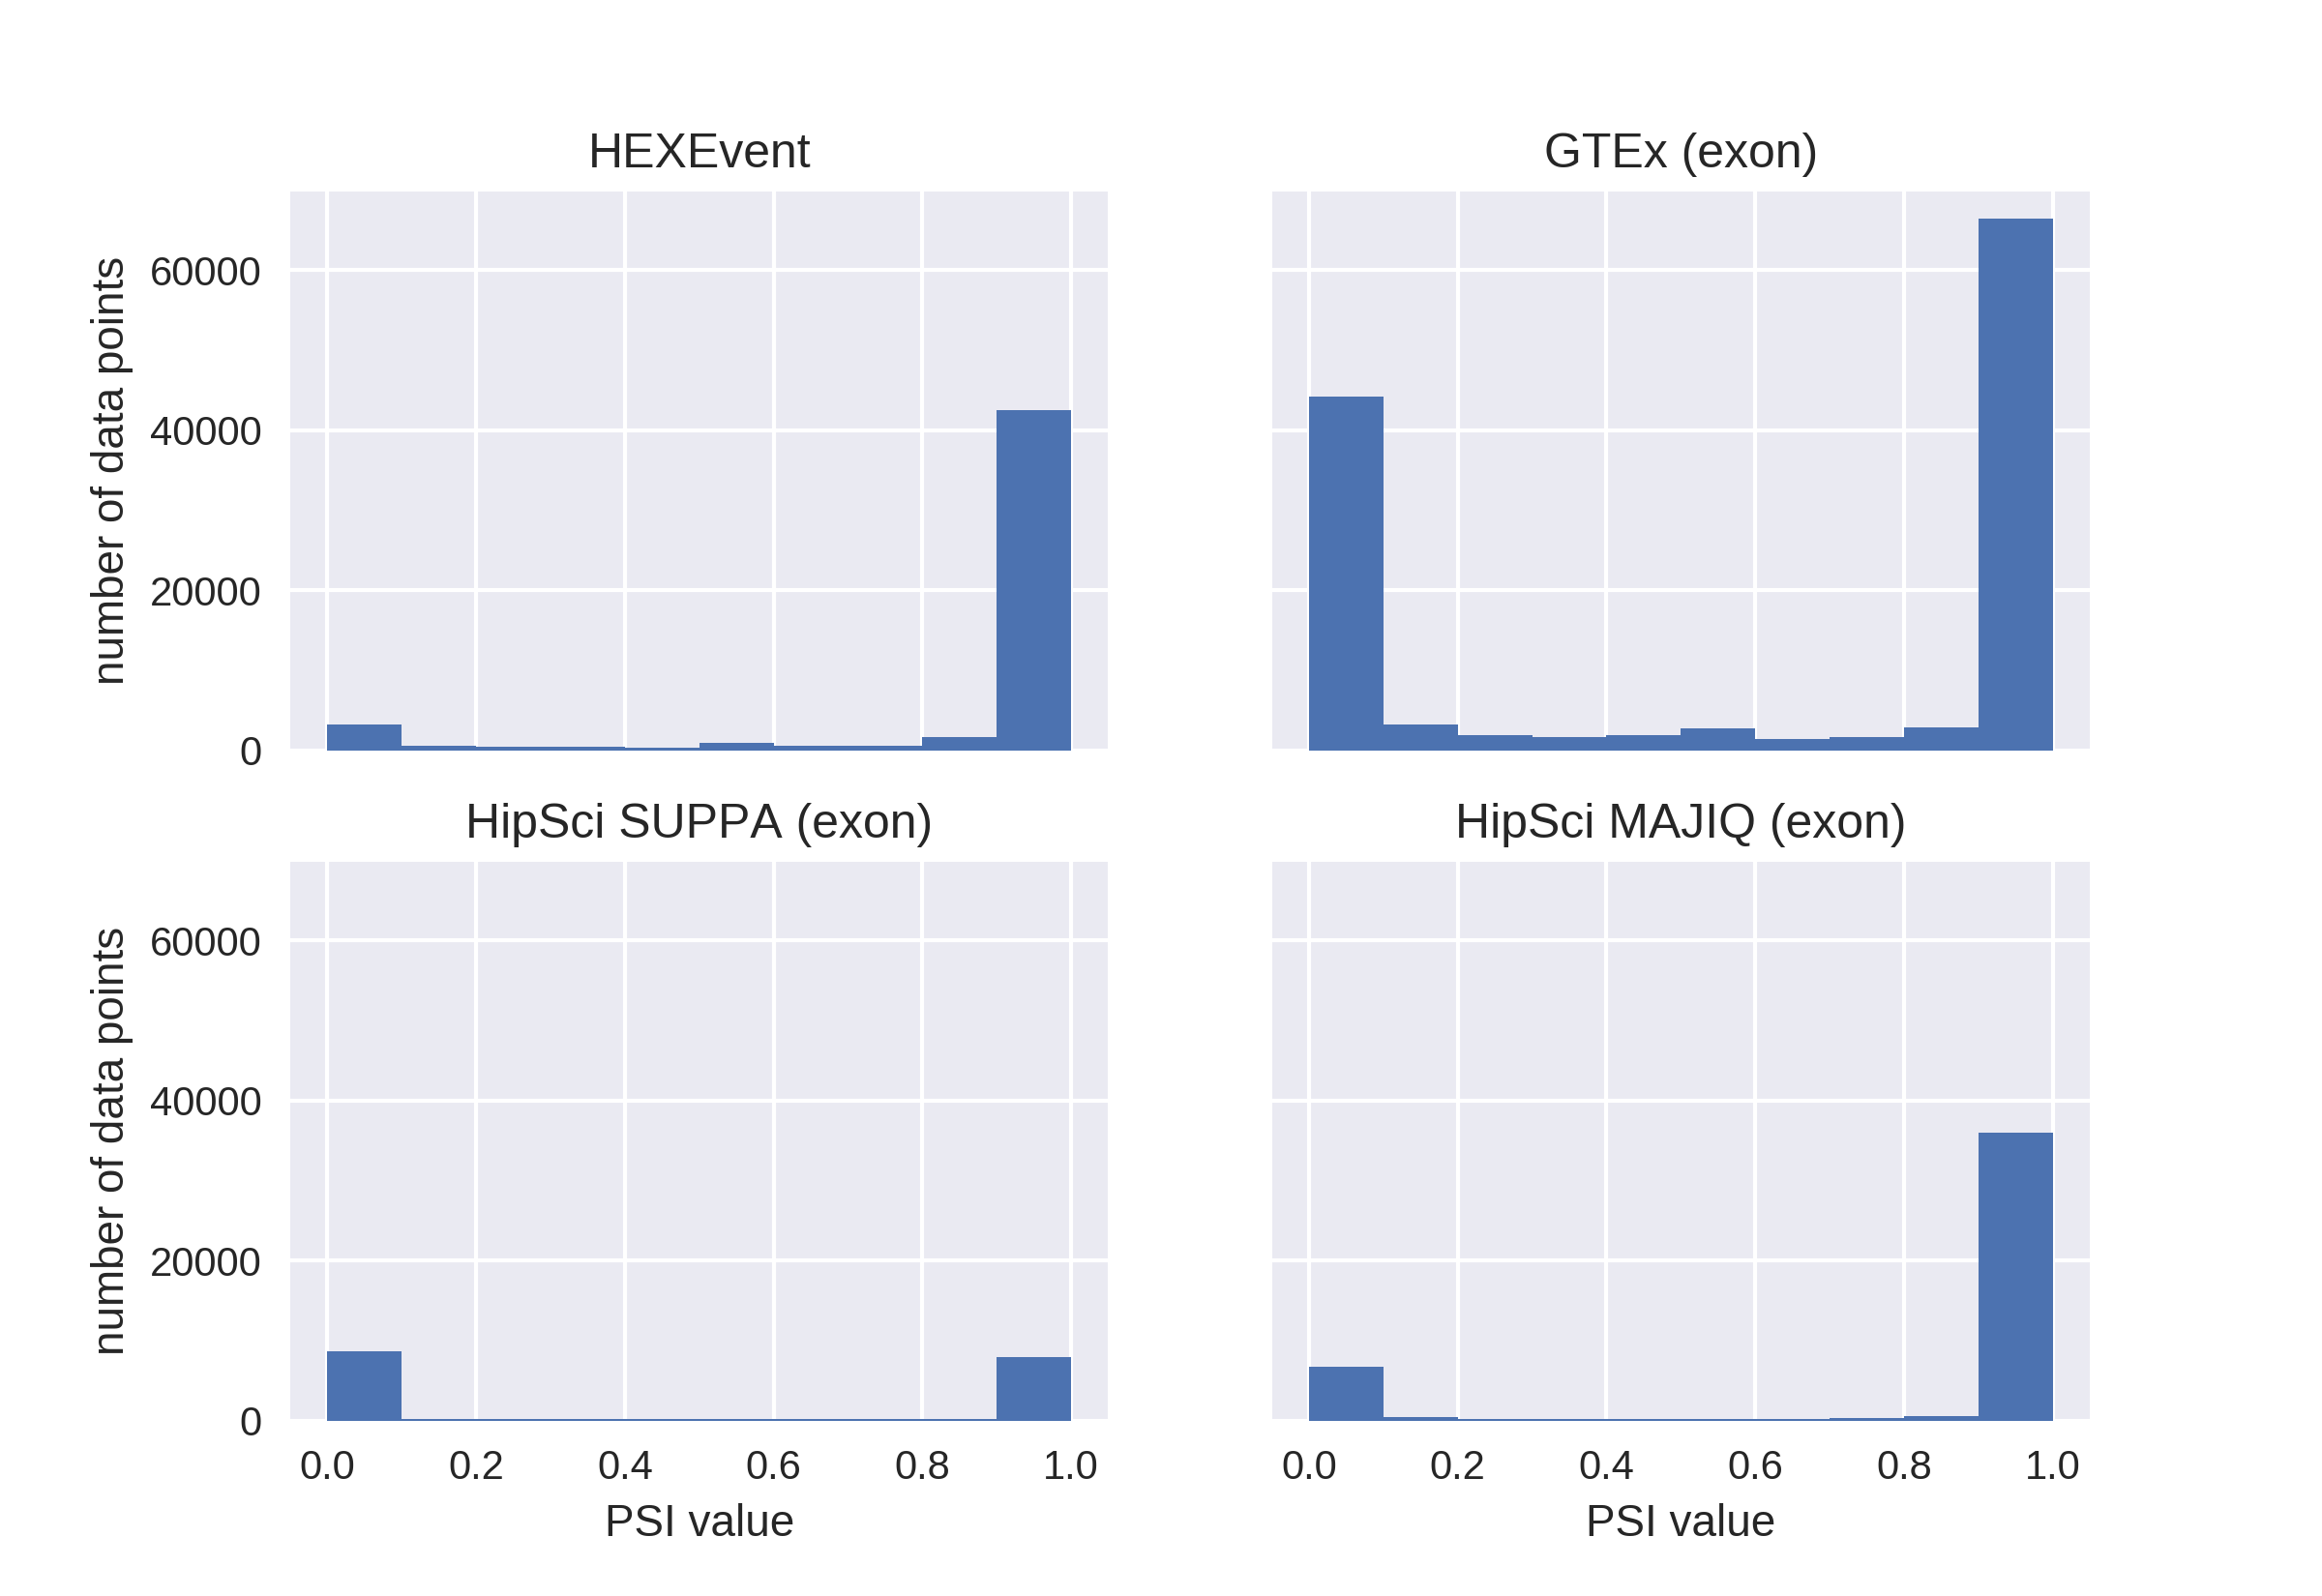
\includegraphics[width=0.7\textwidth]{../visualizations/dataset_histograms_seaborn.png} 
	\caption[test.]{
		...
	}
	\label{fig:datahistograms}
\end{figure}

Figure \ref{fig:datahistograms} shows histograms for the exon-centric version of the four primary datasets versions. The histograms show that the distribution of PSI values is bi-model with the modes being around very rarely included (< 5\%) and very frequently included exons (>95\%). However, there are also some dissimilarities between the datasets: the GTEx and HipSci SUPPA dataset contain the fewest samples and, in particular, they contain significantly fewer constitutive samples.\\
The biggest contributor to this is that due to their respective processing methods the GTEx and HipSci SUPPA datasets only contain known cassette exons as constitutive exons, but not non-cassette constitutive exons. Another factor is that they only estimate PSI based on one biological sample in contrast to the other datasets. HipSci SUPPA especially has an extremely low number of non-rarely or frequently included exons which is likely an artefact of its coarse, transcription-level estimation method.\\
%The relatively low number of non-constitutive exon samples in the HEXEvent dataset is likely influenced by the ESTs coming from a mix of biological samples from different tissues. Among many tissues, there are likely few tissues that contain some exons
%should also hold for constitutive exons; so rarely exons constitutive, so more with middle psi values
%SCEPTICAL -- unlikely to include
%todo:
%collecting average l2 lengths of datasets
%gtex: 24.81448218801441 +- 93.86430163002234
%realization: don't I just collect cassette exons? :o what about vanilla constitutive exons?
\section{Models} \label{sec:models}
The models are fundamentally all split into two components. \\
The first component extracts the most relevant features of the two input sequences of nucleotides. The feature extraction for the sequence around the exon start and the exon end is done independently. Depending on the exact model, the feature extraction is based either on CNNs, BiLSTMs or MLP. The extracted features of this layer are concatenated along with the length features and fed as input to the second component.
The second component uses the extracted features and length features to perform binary classification. This component is implemented as a shallow MLP for all models. It consists of one or two fully connected layers followed by dropout and activation layers. A sigmoid activation function is used after the last layer to obtain an output from [0, 1].
\subsection{DSC: CNN-based} \label{subsec:dsc}
This model is the same as the Deep Splicing Code (DSC) model from \cite{dsc} and is based on CNNs.
CNNs are useful when the input data contains spatially invariant patterns. Since images are fundamentally made up of small, spatially invariant patterns which can be combined into more complex patterns, CNNs have been extremely successful in Computer Vision.\\
CNNs are also extremely promising for the application to nucleotide sequences: \\
1) We can expect to find motifs in the input sequence. Motifs are often represented as position weight matrixes (PWMs). The kernels used in CNNs can be interpreted as PWMs with learnable weights, i.e., the model can automatically learn to recognize important motifs.\\
2) These motifs may be found at different positions in the input sequence. Due to CNNs being spatially invariant they will be able to detect motifs at any position in the input sequence. \\
Keeping this motivation in mind, the first model extracts features from the two input sequences using CNN-based blocks. A CNN feature extraction block with the same architecture but independently learned weights is used for each input sequence. This is to accommodate the model learning to extract different features from the exon start and exon end sequence. The extracted features are used by a shallow MLP to obtain the final classification. 

Concretely, a CNN block consists of three convolutional layers. The first convolutional layer has a window size of 7 units and 32 filters, the second has a window size of 4 units and 8 filters and the third has a window size of 3 units and 8 filters. Each convolutional layer is followed by a dropout layer with dropout probability 0.2 to reduce overfitting [cite dropout], a ReLU activation layer and a max-pooling layer with stride and window size 2 to extract the most salient features. The hyperparameters for this model were chosen with grid search by \cite{dsc}. As we are dealing with inherently 1-dimensional textual data instead of inherently 2-dimensional image data, 1D convolution layers are used.

%https://stats.stackexchange.com/questions/288261/why-is-max-pooling-necessary-in-convolutional-neural-networks
%no one knows why max-pooling works

The extracted features for both genomic sequences are concatenated along with the normalized exon and flanking introns and input to a fully connected layer with 64 neurons. A ReLU activation function, as well as a dropout layer with probability 0.5, is applied to the output of this layer. The final layer takes in the 64 outputs from the previous layer, predicts a single value and is followed by a sigmoid activation layer.
a word on 1d convolution?
\subsubsection{Applying NLP techniques to genomic data}
Like text, genomic data is fundamentally a sequence of characters.
This makes it possible to apply techniques known from Natural Language Processing (NLP) to genomic data. This is an especially promising area of cross-pollination because of the large strides NLP has been able to make in recent years using deep learning.
Some of the most important milestones in NLP have been efficient embeddings via word2vec, applying RNNs to text as in seq2seq and extremely powerful and deep Transformers.
In this work, we will test the application of doc2vec (a derivative of word2vec) and seq2seq models to the task of alternative splicing classification. The current state-of-the-art transformer models, albeit very potent, usually require huge datasets in the order of millions of samples which aren't available for this task. While scaling them down might be an interesting avenue of research even heavily scaled-down models might still be over parametrized for the task as it has frequently been shown that very shallow networks (with less than 5 layers) perform best on genomic data. Additionally, our input sequences are very long; generally 140 tokens long. Initial tests showed that this also leads to memory problems when training on only one GPU, as the memory requirements of Transformers grows quadratically with respect to the length of the input sequence, further complicating their application. Due to these considerations, we chose to forego the evaluation of Transformer-based models in this study.
\subsection{D2V: MLP-based} \label{subsec:d2v}
%If I want to expand this section:
%Asgari, E., & Mofrad, M. R. (2015). Continuous distributed representation of biological sequences for deep proteomics and genomics. PloS one, 10(11), e0141287.
%Contains very good explanations / phrasings
\subsubsection{Introduction to word embeddings}
Word2Vec is a neural network-based model from Natural Language Processing (NLP) which provides a continuously distributed (vector) representation for each word within a sentence \cite{w2v1}\cite{w2v2}. The main idea of Word2Vec is that the meaning of a word is characterized by its context and therefore semantically related words will be similarly represented. The classic example is that

%Distributed representation has proved one of the most successful approaches in machine learning [6–10]. The main idea in this approach is encoding and storing information about an item within a system through establishing its interactions with other members. [biobvec]

King - Man + Woman ~= Queen
vector arrow over words would be great
when adding the Word2Vec representations of the respective words.
Doc2Vec is an extension of Word2Vec which can handle variable length texts (such as paragraphs and complete documents) \cite{d2v1} \cite{d2v2}. It returns a fixed-length representation independent of input size.

\subsubsection{Training}
To train word2vec or doc2vec a large corpus of unlabelled data is needed. As we are training on genomic data, the largest corpus is the complete genome itself. The complete human reference genome GRCh38 was obtained from UCSC. [http://hgdownload.soe.ucsc.edu/goldenPath/hg38/chromosomes/]
During training on text data, the corpus is split into documents which are ideally semantically meaningful (like paragraphs). Due to memory limitations and due to corresponding to the average gene size \cite{bionumbers}, we split the genome into sequences of 28,000 nucleotide sequences. However, tests with sequences of length 10,000 showed that this boundary length does not seem to affect model performance in a meaningful way.
\subsubsection{Using k-mers}\label{subsubsec:kmers}
Naively applying word2vec or doc2vec to genomic data would mean treating each nucleotide as a token. Drawing the parallel to natural language, this would mean wanting to embed each character in a word. However, a single character or nucleotide (which on top comes from an alphabet of only four characters) does likely not contain enough information by itself. Therefore, it is desirable to embed a k-mer.
One major difference between text and genomic data is the single-token complexity: a word contains far more information than a single nucleotide.
Multiple studies have explored this issue and found 3-mers to perform the best. [add quotes from IEEE, IEEE itself] We follow their recommendation in this work and split each sequence of nucleotides into overlapping 3-mers. Overlapping means that in the case of the sequence 'AACGAT' the resulting overlapping 3-mer sequence is 'AAC', 'ACG', 'CGA' and 'GAT'. Therefore, the 28,000 nucleotides long pre-training sequences are split into overlapping 3-mer sequences (sentences) of length 27,998.
\subsubsection{Pre-training of word embeddings}
The pre-training for word2vec uses a shallow neural network with an input, hidden and output layer. If the continuous bag-of-words technique (CBOW) is used, all words in a window except the current word are given as input and the target output is the current word. Typical window size is 5. [WHAT DOES THE HIDDEN LAYER LOOK LIKE? -- could honestly skip this]
If the skip-gram technique is used, only the current word is given as input and the task is to predict the surrounding words in the window. Doc2Vec works similarly. In the CBOW equivalent called distributed memory (DM), a document identifier (usually just an integer enumerating all documents) is given as additional input. In the skip-gram equivalent distributed bag of words (DBOW), the current word is replaced by the document identifier and the task is to predict all words in the window. All four different training methods are visualized in Figure [figure 3 from distributed].
There is no clear choice for when which training method should be used for Word2Vec or Doc2Vec as the training methods tend to perform similarly. However, DM (and also CBOW) preserve the order of words and as the order of words (3-mers) is likely significant, we chose DM as pre-training method.
Pre-processing the human genome like above and using the DM training method, we trained the Doc2Vec model to output a 100-dimensional embedding for each document.
\subsubsection{Analyzing the obtained embeddings}
We visualize the embeddings for all 64 possible 3-mers using Stochastic Neighbor Embedding (t-SNE) [36] in Figure [t-SNE embeddings; both w/ nts and w/ amino acids].
%TODO tSNE citation
Doc2Vec is trained to map words (3-mers) which occur in a similar context to similar representations. We observe that this often translates to mapping the same amino acids to similar representations. There are some instances when different amino acids are mapped together like the quartet Ala, Thr, Pro and Ser in the top-left corner. Displaying the 3-mers associated with the amino acids, that this likely occurs because these different amino acids share two out of three nucleotides at the same positions. We take this visualization as an indication that Doc2Vec was able to learn biologically useful embeddings for the overlapping 3-mers.
[maybe] Making use of these pre-trained embeddings, each 140 nucleotide input sequence is split into overlapping 3-mers and mapped to a 100-dimensional vector. Like in the other models, a shallow MLP using these sequence features in conjunction with length features for classification.
Inference:
During inference, the Doc2Vec model outputs 100-dimensional embeddings for each input sequence. These, along with the length features, are fed into the shallow MLP for classification. The shallow MLP consists of two layers with 16 and 8 neurons each respectively followed by a dropout layer with dropout probability of 0.2.
%TODO ![](https://lh5.googleusercontent.com/iapyd6dbrKCN6Y8HzSUDi7fNx5XlgKbCHvZj6Y6J6CRCF4_PTS527lgO9-R_NVPthwxGQrq1DNBEwXfVZqjyXtdf_UmVW8MgYv6zSOJsauefzy9X5HQJI9lF30QBk-a7uLc7DT0N)
[discussion of the tsne embeddings here]
research on what to write:
doc2vec will map words (3-mers) which are used in similar contexts to similar representations
wil: codon usage bias; not all encodings of a codon will be used with the same frequency
the bias of codon usage at exon boundaries
Laurence Hurst paper looks at biases in the first and last 30 nucleotides within an exon
\subsection{BiLSTM + Attn} \label{subsec:bilstm}
\subsubsection{Seq2Seq} \label{subsubsec:seq2seq}
Sequence-to-sequence (Seq2seq) Sutskever et al. in 2014, below] is a general deep learning-based framework for mapping one sequence to another. The first part of the framework is an encoder which processes the input symbol-by-symbol and produces a vector representation for each input symbol. The second part is a decoder which predicts the output sequence based on the representation by the decoder. In the first timestep, the decoder uses the last output of the encoder and in all other timesteps, it uses its output from the previous time step as input. The encoder and decoder are typically RNN-based networks such as LSTMs [schmidhuber] or GRUs [quote GRU]. Encoder and decoder are jointly trained to maximize the probability of correct output. This framework has been particularly successful in machine translation (MT): for instance, Google announced in 2016 that it started using them for their MT. Figure ![ visualizes the working of an encoder-decoder model.
%TODO Sutskever, I., Vinyals, O., & Le, Q. V. (2014). Sequence to sequence learning with neural networks. In Advances in Neural Information Processing Systems.
%https://smerity.com/articles/2016/google_nmt_arch.html
%https://ruder.io/a-review-of-the-recent-history-of-nlp/index.html#2013wordembeddings
\subsubsection{Are you paying attention?}
In the original Seq2seq framework, only the last state of the encoder is passed to the decoder. This means that the encoder needs to encode all of the information observed in the input sequence into its last state. While theoretically possible, [ICLR] hypothesized that this informational bottleneck hampered performance in practice. They proposed removing this bottleneck via introducing attention. Attention is a mechanism whereby the decoder can look at all the representation generated by the encoder at once and can 'choose' to focus on the most important ones. Introducing attention lead to large performance gains across Seq2seq-based models and quickly became standard practice. The attention mechanism also adds interpretability to the model because it indicates which parts of the input sequence are most crucial for the model's prediction. Figure [] visualizes what parts of an input sequence a model is paying attention during an MT task. Attention is one of the most important innovations in deep learning research in recent years. For instance, the current state-of-the-art Transformer models [bert, aiayn] forego recurrent networks completely and solely use attention within the encoder and decoder components.
However, as justified earlier, we won't focus on these models due to issues of scaling and the sufficiency of shallow networks for genomic prediction tasks.
%TODO Bahdanau, D., Cho, K., & Bengio, Y. (2015). Neural Machine Translation by Jointly Learning to Align and Translate. In ICLR 2015.
could also use graphics from this
%another attention reference: https://arxiv.org/pdf/1508.04025.pdf
%https://3.bp.blogspot.com/-3Pbj_dvt0Vo/V-qe-Nl6P5I/AAAAAAAABQc/z0_6WtVWtvARtMk0i9_AtLeyyGyV6AI4wCLcB/s1600/nmt-model-fast.gif
%alternative: https://machinetalk.org/2019/03/29/neural-machine-translation-with-attention-mechanism/
Attention is a very general mechanism not limited to the Seq2seq framework and different forms of it (such as additive [bengio original] or multiplicative attention [transformer]) are used in practice. It can theoretically be useful for any task where a model needs to make a decision based on certain parts of an input.
%[transformer here and why I don't use it]
%[More applications of attention]
%It has been applied to constituency parsing (Vinyals et al., 2015)
%, reading comprehension (Hermann et al., 2015)
%, and one-shot learning (Vinyals et al., 2016)
%, among many others. The input does not even need to be a sequence but can consist of other representations as in the case of image captioning (Xu et al., 2015)
%, which can be seen in Figure 12 below
\subsubsection{Integrating attention}
Taking inspiration from the successful application and improved interpretability of the Seq2seq framework with attention in other domains, we also want to apply it to constitutive exon classification. We now describe the modifications we made to be able to use this set up in our context. In particular, we describe the attention mechanism in more detail as necessary for our second modification.
\subsubsection{Modification 1: MLP instead of a recurrent decoder}
As the name implies, models based on the Seq2seq framework take a sequence as input and give a sequence as output. This is achieved via using a recurrent decoder which outputs symbols until it outputs an <EOS> (end-of-sentence) token (in the case for MT, similar for other domains). However, in our case, the output will always be a single scalar: the classification of the exon as constitutive or alternatively spliced. Thus, we don't require a recurrent decoder and instead use a shallow MLP for classification of the encoder features.
\subsubsection{Modification 2: Attention with a learned query vector}
The most common form of attention (multiplicative or dot-product attention), makes uses of conceptual queries and key-value pairs. A given query is compared to all keys by computing a similarity score between the query and each key via the dot-product. The similarity scores are normalized through the use of a softmax layer. The normalized similarity scores are also commonly called the attention weights; keys similar to the query are weighted more. The output of the attention layer for a given query and input sequence is then the weighted vector sum obtained by multiplying each value by the attention weight of its respective key.
Putting the above intuition into formulas, the (dot-product self-) attention mechanism can be described using the following equations:
$$Q, K, V = IW^Q, IW^K, IW^V$$
The query, key and value matrices Q, K and V are computed by multiplying the input with query, key and value parameter matrices $W^Q$, $W^K$ and $W^V$.
where $$W^Q,W^K, W^V \in \mathbb{R}^{in \times out}$$,
and $$Q,K, V \in \mathbb{R}^{l \times out}$$. in corresponds to the number of features of each element in the input sequence to the attention layer, out corresponds to the number of features in the output of the attention layer. l corresponds to the number of elements in the input sequence to the attention layer.
Attention can be then computed as:
$$Z = attention(I) = softmax(QK^T)V$$
where $$Z \in \mathbb{R}^{l \times out}$$. The input I is a concatenation (along the first dimension) of the representations given by the two BiLSTMs.
This makes use of the fact that $$Q\cdotp K = QK^T$$ where $$\cdotp$$ denotes the dot product.
%This form of attention is also visualized in Figure !](https://jalammar.github.io/images/t/self-attention-matrix-calculation.png) and ![
%from https://jalammar.github.io/illustrated-transformer/
%todo: remove this division by square-root -- maybe ask Kuba how to photoshop this away
As shown, multiplicative self-attention computes a separate query for each input token. It is called self-attention because it allows a sequence to pay attention to 'itself'. (Unmasked) self-attention is mainly used in the encoder part of Transformer architectures to improve the representation for each word.
However, our objective in using attention is not to improve the representation for each symbol in a sequence (this is the task of the BiLSTM), but to select the most important features from an input sequence. The conceptual query for our task is also always the same independent of input: is this exon constitutively spliced or not?
%thought: this also naturally happens in seq2seq models when they use attention -- how is what I am doing differently?
Thus, we adapt the attention mechanism so that we learn a single, input-independent query $${Q}^* \in \mathcal{R}^{1 \times out}$$. The output of the attention layer is now computed as:
decided against explaining innovation as two-points with (1) one query and (2) independent of input because I felt unsure of (2)
$$Z^* = {attention}^*(I) = softmax({Q}^*K^T)V$$
where $$Z^* \in \mathbb{R}^{1 \times out}$$. Note that the query matrix $${Q}^*$$ is directly learned in the attention block and not multiplied with the input, giving rise to its input independence. The output Z is now a weighted sum of the nucleotide representation in the input sequences which the model deemed most crucial to pay attention to.
\subsubsection{Putting it all together:}
Like a Seq2Seq model, an RNN-based Encoder is used to capture a representation of the input sequence. We select the most important representations of the input using the modified attention mechanism we introduced. Instead of a recursive decoder, we use a shallow MLP for classification based on the selected features.
One detail not mentioned yet is that the input to the BiLSTM blocks is a dense 4-dimensional embedding of the one-hot encoded sequences. This embedding is the same for each sequence and jointly learned during training. This extra embedding layer is included as previous works have shown that otherwise, the model might suffer from limited generalization performance caused by the sparsity of the one-hot encoded representation. 
%todo: [https://arxiv.org/pdf/1512.05135.pdf]
\subsection{Alternative implementations of attention}
In the following, we introduce multiple extensions which were attempted which didn't lead to improved results. For most of these, initial results clearly showed that the results weren't improved by using them. As such, we didn't test these extensions more extensively than initial experiments because we felt the initial results were already instructive enough and no further investigation was warranted. Thus, the analysis of the results won't be as extensive as for the extensions which worked.
\subsubsection{No query}
As the query matrix $${Q}^*$$ is already the same independent of the exact input sequence, it could be possible to drop it and compute the attention weights sorely based on the key matrix K.
This is possible by learning a key weight matrix $$W^{K^*} \in \mathcal{R}^{in \times 1}$$ and computing attention as:
$$K^* = IW^{K^*}$$
$$Z^{} = {attention}^{}(I) = softmax(K^*)V$$
where $$K^* \in \mathbb{R}^{l \times 1}$$ and $$Z^{**} \in \mathbb{R}^{1 \times out}$$
However, in initial experiments, the attention** mechanism performed significantly worse than the attention* mechanism. The extra representational capacity by having a query matrix seems to be important for performance.
\subsubsection{Multiple attention heads}
Having one set of query, key and value matrices limits the model to one representational subspace (one way of 'interpreting' the input). It might be useful for the model to have multiple representational subspaces. This is usually achieved via $$h$$ different sets of query, key and weight matrices $$W^Q_1, W^Q_1, W^Q_1, \dots W^Q_{h}, W^Q_{h},W^Q_{h}$$ producing multiple outputs $$Z_0, \dots, Z_{n\_h}$$.
The final output matrix $$Z_{final} \in \mathcal{R}^{l \times out}$$ is then computed as:
$$Z_{final} = concat(Z_1, \dots, Z_{h}) W^O$$
where the concatenation occurs along the second dimension and $$W^O \in \mathcal{R}^{out * h \times out\_new}$$
thought: might change this up a little, would require a bit more implementation effort than previously thought (eg. initial attention dimension should be divided by 3) or requires the assumption that out == $out_new$ (I think I will choose this one, but not certain)
\subsubsection{Convolution in attention heads}
As was previously discussed in the motivation for splitting the input sequence into overlapping 3-mers in \ref{subsubsec:kmers}, the information contained in a single nucleotide is very low. This motivated [ghent bio transformer paper] to apply an additional 1D convolution to the query, key and value matrices Q, K and V. This extension can be understood as an alternative to splitting the input into k-mers and provided better results than splitting the input into k-mers when using a Transformer network for a genome annotation task in [].
Keeping in mind the modification of directly learning the query matrix, this leads to:
$$K_{conv}, V_{conv} = conv(K), conv(V)$$
$$Z^* = {attention}_{conv}^*(I) = softmax({Q}^*K_{conv}^T)V_{conv}$$
where the K and V are both fed through the same convolutional layer.
The number of convolution filters and padding are chosen so that the dimensions of the K and V matrices don't change, that is, $$K_{conv}, V_{conv} \in \mathbb{R}^{l \times out}$$.
One more detail regarding the application of this extension: to incorporate the domain knowledge that the input sequences to the neural network come from different places in the genome, we made sure that the convolution did not mix the information between the two sequences. To achieve this, the following computation actually took place :
$$K^{start}, K^{end} = I^{start}W^K, I^{end}W^K,$$
$$K^{start}_{conv}, K^{end}_{conv} = conv(K^{start}), conv(K^{end})$$
$$K_{conv} = concat(K^{start}_{conv}, K^{end}_{conv})$$
where the 'start' and 'end' superscript respectively refer to the sequence around the start and end of the exon. The concatenation is along the first dimension (so the length of the sequences). The analogue computation was done for $$V_{conv}$$.
Testing this extension on the HipSci MAJIQ dataset didn't lead to improved results. Although the convergence speed increased rapidly (from around 180 epochs to 20 epochs), we also observed heavy overfitting. To alleviate this, we added dropout and batch normalization layers. After adding two dropout layers with a high dropout probability (one after computing the attention weights and one after the convolution layers with p=0.5 each) and setting the convolutional filter size to no higher than 3, overfitting issues ameliorated. However, after adding these layers convergence was no faster than for the case without convolutional layers and the performance did not improve. Thus, for the sake of a simpler model, we opted to not use this extension for the rest of the experiments.
Reasons for why this extension did not work might be related to the use of a recurrent encoder as well as task differences compared to [ghent].
\begin{enumerate}
	\item Although we process the input at single-nucleotide resolution, the use of a BiLSTM means that the encoder is aware of the nucleotides which precede and follow it. Therefore, information about the neighbouring nucleotides is likely already represented in the representation for a given nucleotide. This is in contrast to a Transformer model where the layers are non-recurrent and only work at single-symbol resolution. Thus, the convolutional layers likely don't give the model a lot more flexibility.
	\item In [], the task is a full genome transcription start site annotation. Therefore, in a sense, their task occurs at the inter-gene level while our task occurs at the intra-gene level. This likely means that the motives the model has to consider generally span more nucleotides and giving the model more capacity to integrate over multiple nucleotides is more crucial. In contrast, the single-nucleotide resolution of our model may be necessary to help it identify the more fine-grained motifs which influence splicing. Thus, these differences likely also influenced the performance differences when using the convolutional attention layer extension in the different models.
		they: 3000 nucleotides, convolution filter of 7
\end{enumerate}


A small implementational detail regarding the attention blocks: the query, key and value parameter matrices are implemented via a linear layer with the appropriate dimensions. These also learn bias weights which are added to the output by default. While in theory the bias weights should be turned off to implement exactly the shown formulas, in practice other attention mechanism implementations leave these turned on [annotated transformer] and so we follow suit. Thus, to be precise, the query, key and value computation should be:
%TODO
%   old motivation:
%The architecture of this model can be motivated in two ways:
%1) Similar to DSC, we use two blocks for feature extraction. However, incorporating the knowledge that our input data is a sequence, we use an RNN for this feature extraction. In particular, under the assumption that bidirectional context is important for this task, we use bidirectional LSTM (BiLSTM). Like DSC, a shallow MLP uses the obtained features of both blocks for classification.
%2)
%The final model is very similar to the current state-of-the-art splicing code for predicting the inclusion rate of a cassette exon [distributed], as introduced in [related works].
%maybe: (could make my motivation seem shallow)
%This is a standard LSTM architecture and a similar architecture have been successfully applied to the related task of finding new splice junctions. [https://arxiv.org/pdf/1512.05135.pdf, https://www.sciencedirect.com/science/article/pii/S0010482519304135]
%simple feature extraction + classification model as eg in [https://www.researchgate.net/figure/An-example-of-bidirectional-LSTM-tagger-architecture_fig1_330276457 ] -- 5 citations

For this model, the hyperparameter space was a lot larger and model performance was very sensitive to the hyperparameter choice. The most crucial hyperparameters were the number of encoder dimensions and the number of dimensions of the attention layer. Hyperparameters were optimized via grid search on the HipSci MAJIQ dataset.
putting model parameters into the text instead of a table:
Concretely, each LSTM block consists of a BiLSTM with one (?) layer which outputs 50 features.
The shallow MLP used for classification uses a single layer with 128 (?) neurons and is followed by a dropout layer with dropout probability of 0.5.
mention respective model sizes here
bilstm 93261, dsc 20.001, d2v 3281 [postponed until I have settled on them]
could also put them in table and compare later

\section{Training and implementation details}
\subsection{Implementation}
% TODO: include figures from overleaf
All models, except the Doc2Vec network, were implemented using the PyTorch library (version 1.5.0) \cite{pytorch}. The Doc2Vec model was implemented using the gensim library (version 3.8.3) \cite{gensim}. The data processing was done using a mixture of Python and Bash scripts as well as the software tools MAJIQ and SUPPA described in section \ref{subsubsec:majiq} and \ref{subsubsec:suppa}. The complexity induced by the use of a large number of different datasets and data processing methods was handled by standardizing the shape of the final training samples. Even though 12 different dataset variants and 4 different models are used, the codebase contains only 2 different data loader and trainer classes.\\


The structure of the repository was based on the PyTorch Deep Learning Project template available at \url{github.com/victoresque/pytorch-template}. This template provides access to abstract classes for data loaders, trainers and the models themselves. These abstract classes already contain a lot of the implementation-independent code to log results and train and save models. These abstract classes can then be extended with implementation-specific code as e.g. exact data formats. Using this structure avoids the duplication of a lot of boilerplate code.\\
To run an experiment, the experimental settings are defined in separate JSON files. This allows for easy and unambiguous reproduction of results. All experiments for whom results in this study are shown are available as JSON files that define the exact parameters used.
The code repository itself contains multiple README which go into more details towards the structuring and using of the code and also define naming conventions.\\

total code base contained roughly ... lines of code. the majority of these were in preprocessing section [maybe exclude this]
\subsection{Training}
The training was done using one NVIDIA GeForce GTX 1080 Ti GPU. This proved to be sufficient as initial exploratory experiments showed no advantage of using deep networks and the resulting networks used are all relatively shallow. The pre-training of the Doc2Vec model on the human genome took 3 hours. We randomly split each dataset into 10 folds; in a given run, 8 folds were used for training, 1 fold for validation and 1 fold for testing. Each model was trained with different folds 9 times.
The training time for training a single model once varied between 1 minute and 25 minutes (see [table with training times]). The models were trained with early stopping on the validation fold until they stopped improving for 15 epochs. This typically occurred after 70 - 150 training epochs.
Where we established in a base experiment that the variance for a given model was low between runs (lower than ~1%), we only trained the model in follow-up experiments once for practical reasons.
\subsubsection{Loss}
All models were trained to minimize the binary cross-entropy loss:
$$\mathbb{L} = - (y log(\hat{y}) + (1 - y) log (1 - \hat{y}))$$
where the ground truth $y \in \{0, 1\}$ and the prediction of the model $\hat{y} \in [0, 1]$. The binary cross-entropy is the standard loss for training deep learning-based (binary) classifiers.
\subsubsection{Metrics}
As in previous work \cite{dsc}, we evaluate all models using the Area under ROC curve (AUC). The AUC provides an aggregate measure of performance across all possible decision thresholds.
However, some of our datasets were unbalanced. This may lead to a degenerating behaviour where a model only predicts the majority class. Additionally, only looking at the AUC does not give a good sense of the .... specificity.. recall?
This is not captured by the AUC. \\
Thus, we also evaluated the F1 of our models when working with an unbalanced dataset as in the case of the HipSci-based dataset processed with MAJIQ.
The output of our models is a single, continuous scalar $\hat{y} \in [0, 1]$. As the AUC itself is an aggregate measure across all decision thresholds, we don't need to set it to a certain value that translates the continuous prediction into a discrete positive or negative class prediction. To compute the F1 score, we do. Naively, this threshold may be set to 0.5; that is, all outputs above 0.5 will be interpreted as a prediction of the positive class and all other outputs as a prediction of the negative class. However, this threshold may not be optimal to maximize the F1 score, especially when working with unbalanced datasets. We choose the threshold which maximizes the F1 score on the test set.


Exact hyperparameters used for training the models are given in table [..]
\chapter{\label{ch:ch5-results}Results}
%3146 words
This section presents and discusses the results of our experiments based on the three models and the datasets introduced in Chapter \ref{ch:4-methods}. It also describes the rationale behind deciding which experiments should be run.

Results are given as obtained on the test set. Across all datasets and experiments, validation and test set metrics differ by less than 1\% on average. We observe no undue overfitting and unless explicitly mentioned, AUCs on the training set are generally higher by 0.02 to 0.06. 
\section{HEXEvent dataset} \label{sec:hexevent_results}
To obtain a baseline, we evaluate all three models on the HEXEvent dataset as used in \cite{dsc} and introduced in \ref{subsec:hexevent}. The results of these experiments are shown in Figure \ref{fig:hexevent_auc}.

\subsubsection{Analysis of main findings}
Generally all models perform extremely well with AUCs nearing 90\%. While differences are small, RASC seems to perform slightly better than the other models.
%They also perform very similarly, making it hard to differentiate them based on their ROC curves. The Attn model seems to perform slightly better than the other models. 

Assessing our reimplementation, we observe a small difference between the AUC value reported in \cite{dsc} (mean 0.899, standard deviation of 0.18) and the ones we observe (mean 0.873, standard deviation of 0.06). This is likely the result of random statistical noise influenced by different random seeds between runs and differences between TensorFlow/Keras (their implementation) and PyTorch (our implementation). Notably, when reevaluating the publically available original implementation in a single run, we also obtain results (0.872 AUC) closer to the results of our reimplementation. 
%There is a small ($\sim$2\%) difference in the AUC values in the AUC values for the DSC model reported in \cite{dsc} (89.9 AUC) and the ones we observe (87.1 AUC original). 
Thus, we conclude that, albeit with minor caveats, the reimplementation and replication of \cite{dsc} was successful.

\begin{figure}
	\centering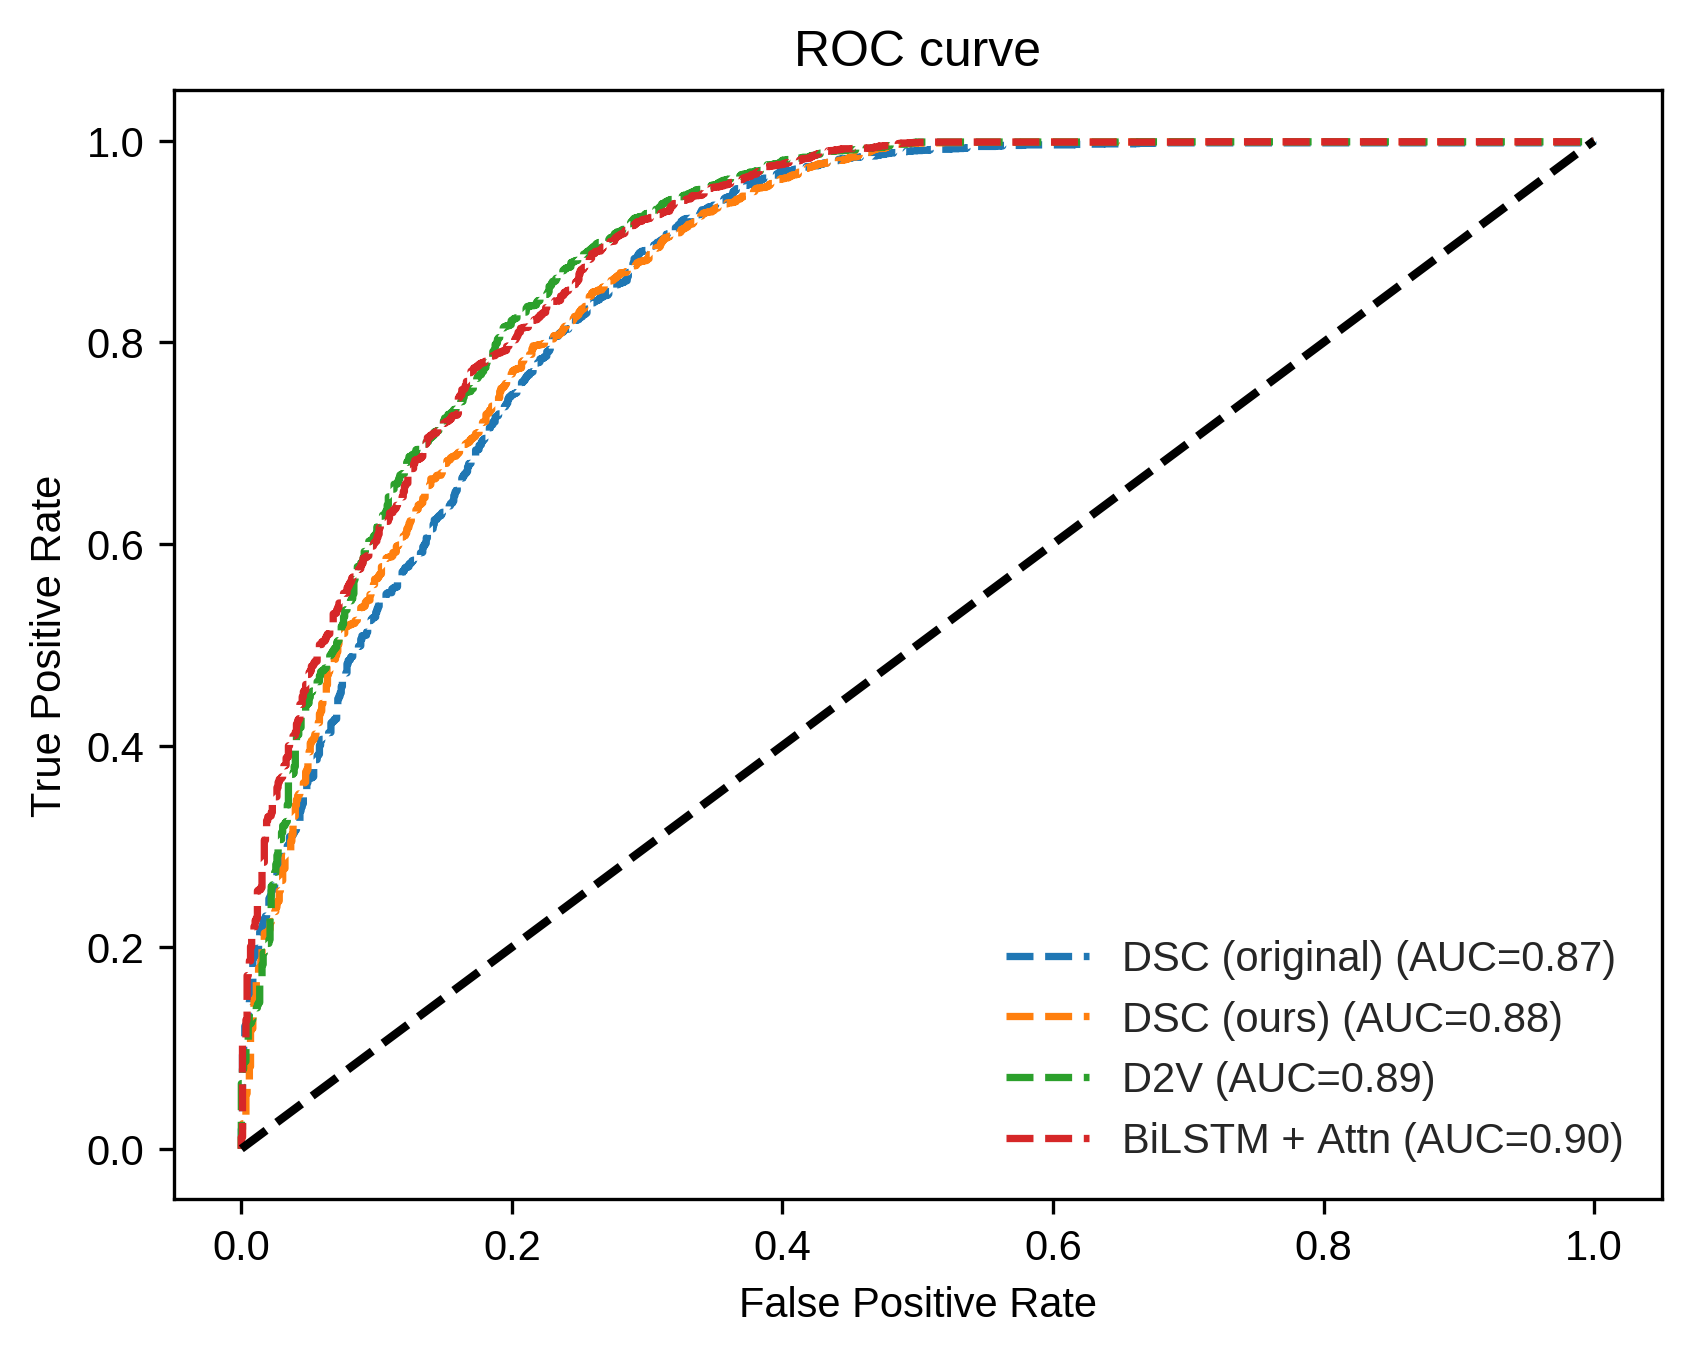
\includegraphics[width=0.7\textwidth]{../visualizations/ch5-results/hexevent_cross_model_roc_auc_comparison.png} 
	\caption{Comparison of the ROC curves of the three models as well as the original implementation on the HEXEvent dataset. The values of the original implementation were obtained by rerunning the training on the publicly available implementation. }
	\label{fig:hexevent_auc}
\end{figure}

%main takeaway: all models perform extremely well \& very similarly



%To showcase the advantage of using the attention mechanism, we also included the BiLSTM-based model where only the last output is used for classification. This model performs significantly worse than the other ones.

% Observation: Performance heavily drops when no lengths feature is used

\subsubsection{Length features are necessary}
Reimplementation was completed piece-wise, that is, first the sequence features were added as input, then the networks were trained to ensure that this was done correctly and then the length features were added. This lead to an interesting observation: model performance is significantly worse when no length features are given to the models. Quantitative results for this observation are given in Table \ref{table:results_hexevent}. This observation is true across models and leads to an average relative performance drop of over 66\%. The information about the secondary structure obtained in the lengths seems to be necessary for the models to obtain good predictive power.

% 0.684, 0.737, 0.663
%0.255, 0.282, 0.268

\begin{table}[h!]
	\centering
		\resizebox{\textwidth}{!}{\begin{tabular}[width=\textwidth]{| l | c | c | c| c} 
			\hline
			Model name & Only sequences & Sequences + lengths & Relative gain\\
			\hline
			DSC & 0.618 & 0.873 & 68.4\%\\
			D2V & 0.614 & 0.896 & 73.7\%\\
			RASC & \textbf{0.636} & \textbf{0.904} & 66.3\%\\
			\hline
		\end{tabular}}
	\caption{Performance of the main models on the HEXEvent dataset with and without length features given as AUC. The relative performance gain (from adding the length features) was computed as $\frac{AUC - AUC_{no\_lengths}}{AUC - 0.5}$. Computing it this way accounts for the baseline AUC of random guessing being 0.5.
	}
	\label{table:results_hexevent}
\end{table}

\subsubsection{Further investigations}
To further investigate, we also test three other models: MLP100, MLP20 and MLPLinear which respectively contain 100, 20 and 20 trainable parameters. The models are MLPs with one hidden layer which only take the length features as inputs. MLPLinear doesn't contain a non-linear activation function after its hidden layer.

\begin{figure}
	\centering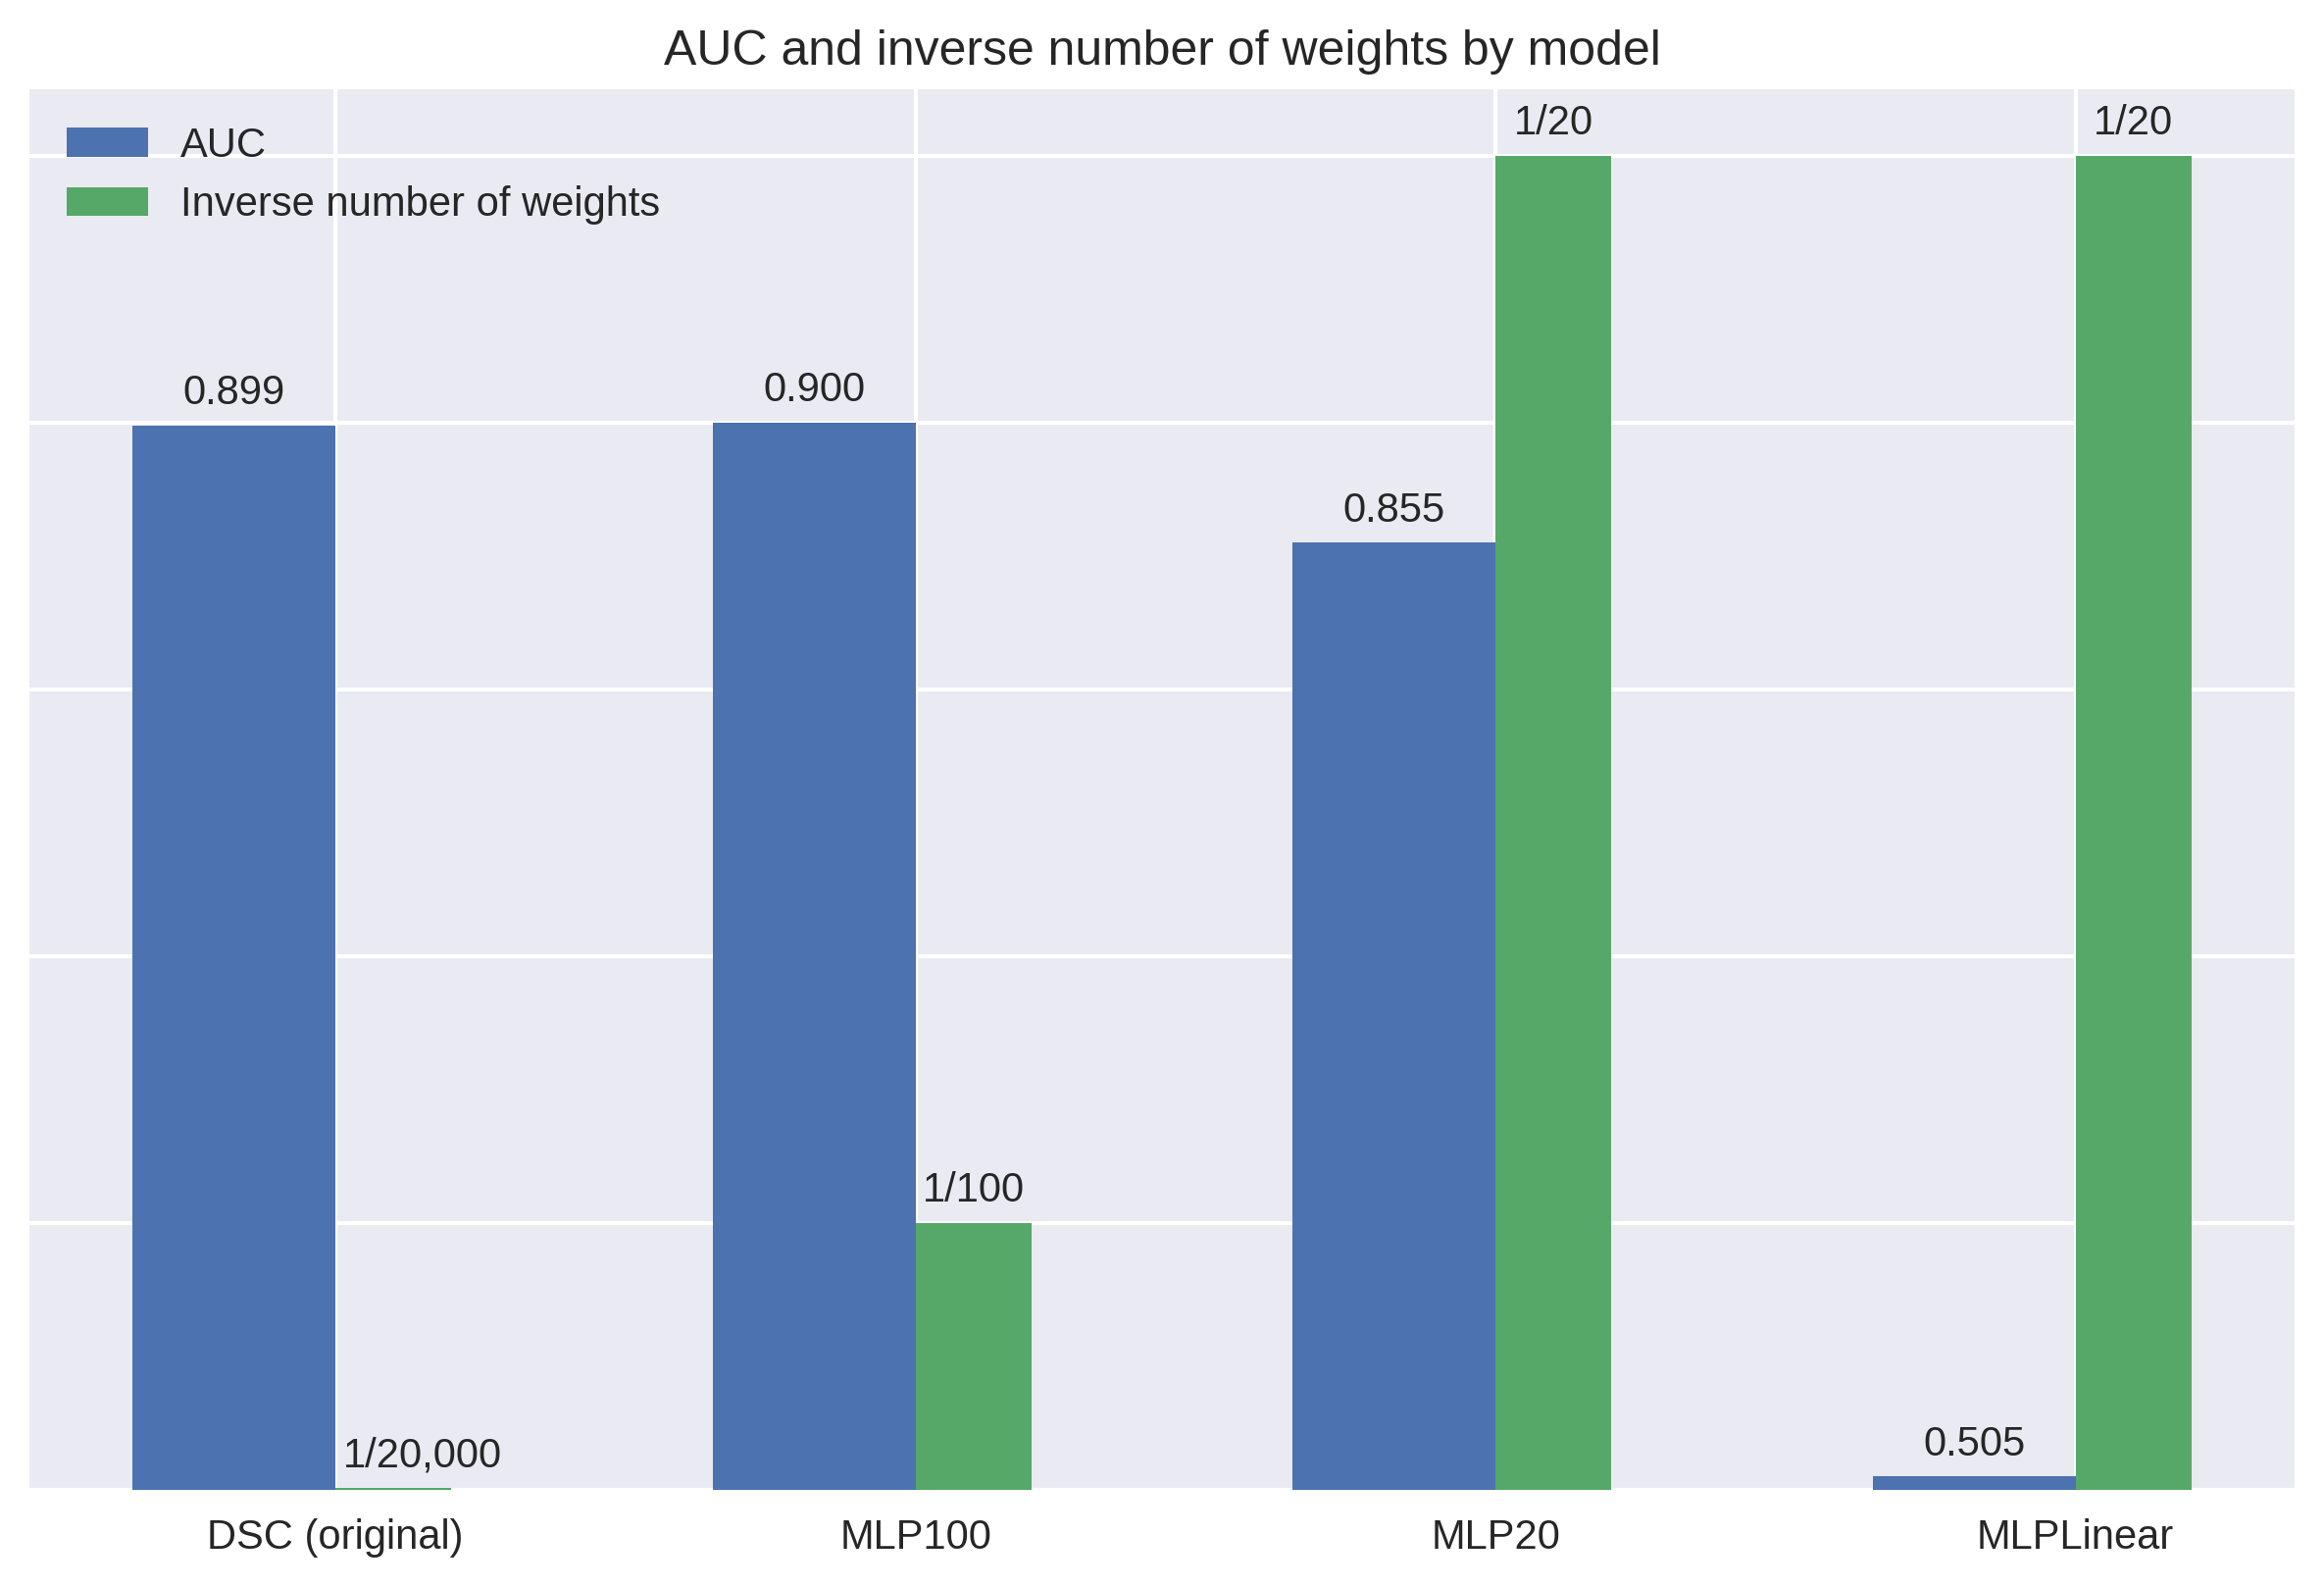
\includegraphics[width=0.85\textwidth]{../visualizations/ch5-results/dsc_funeral_barchart.png} 
	\caption{Stress testing the HEXEvent dataset used in \cite{dsc}. The graph shows the performance as well as the inverse of the respective model sizes used.}
	\label{fig:dsc_funeral}
\end{figure}

Surprisingly, the results in Figure \ref{fig:dsc_funeral} show that it is possible to replicate the results of \cite{dsc} with these very simple models using two to three orders of magnitude fewer parameters (note that DSC has 20,001 parameters). Model performance is improved by adding further parameters and breaks down when no non-linearities are used in the network. This indicates that the models capture a relatively simple, but non-linear relationship between the lengths and the classification of an exon in the dataset. 
There are multiple possible explanations for why this is:
\begin{enumerate}
	\item There are confounders in the dataset learned by the model. As discussed in Section \ref{subsec:hexevent}, EST-based data is inherently biased. The biases inherent in EST-based data could be captured by the exon and intron structure and the model is learning to make its prediction based on this bias. 
%	This explanation is made more likely, if the findings on the HEXEvent dataset don't replicate on the other datasets we evaluate.
	\item Exon splicing is extremely well predictable based on the lengths of neighbouring introns and exons. This is very unlikely given that research into splicing has been ongoing for over 40 years. 
%	This explanation, albeit unlikely already, can be disproven if this observation fails to replicate on other datasets.
	\item There are bugs (e.g. mixing of testing and validation data) in our reimplementation. In the first instance, this is unlikely given that we were able to replicate the original results of \cite{dsc}. To reduce complexity and further reduce the likelihood of a bug leading to these observations, we extracted the complete code for replicating the results of the simple MLP models from \ref{fig:dsc_funeral} into a single file. Additionally, in case of a data leakage bug, the performance of the linear model likely wouldn't break down either. Therefore, we judge bugs in our reimplementation unlikely.
\end{enumerate}

Overall, we conclude that the HEXEvent-based dataset is most likely fundamentally flawed and suffers from confounders.
These findings have significant implications. It calls into questions the meaningfulness of \cite{dsc}'s results, showing the competitiveness of their model. These findings likely also warrant a critical investigation of any other conclusions drawn from papers based on the HEXEvent database. At the time of writing, the HEXEvent paper is cited 34 times. While most of these citations are in passing, multiple papers use a HEXEvent-derived dataset for the training of Machine Learning models such as SVMs \cite{buschhertel}, Random Forests \cite{flawed4} \cite{flawed1}, Decision Trees \cite{flawed2} or AdaBoost-based algorithms \cite{flawed3}. The validity of these papers results' are called into question by these findings.

These data quality issues motivated us to construct alternative, better, datasets. We now give their results.


% many of them, even correlational studies, say that this is a feature, rather than a bug
% how true is this?
% mgith even have to post-pone condemning of HEXEvent dataset until I find a better one 

%Recognition of alternatively spliced cassette exons based on a hybrid model -- confirmed

%A classification of alternatively spliced cassette exons using AdaBoost-based algorithm -- actually says that this is a feature, not a bug

%G2P: Using machine learning to understand and predict genes causing rare neurological disorders --- definitely in some capacity
%Exon size and sequence conservation improves identification of splice-altering nucleotides -- this observation is actually their main contribution
% short exons are more likely to be alternatively spliced


%We showed that the EST-based HEXEvent dataset is likely too flawed to serve as a basis for our methods. Thus, we try to construct an alternative dataset.




%tSNE of MLP embeddings? - nah


\section{GTEx-based datasets} \label{sec:gtex}
\subsection{Exon-centric datasets} \label{subsec:gtex_exon}

\begin{figure}
	\centering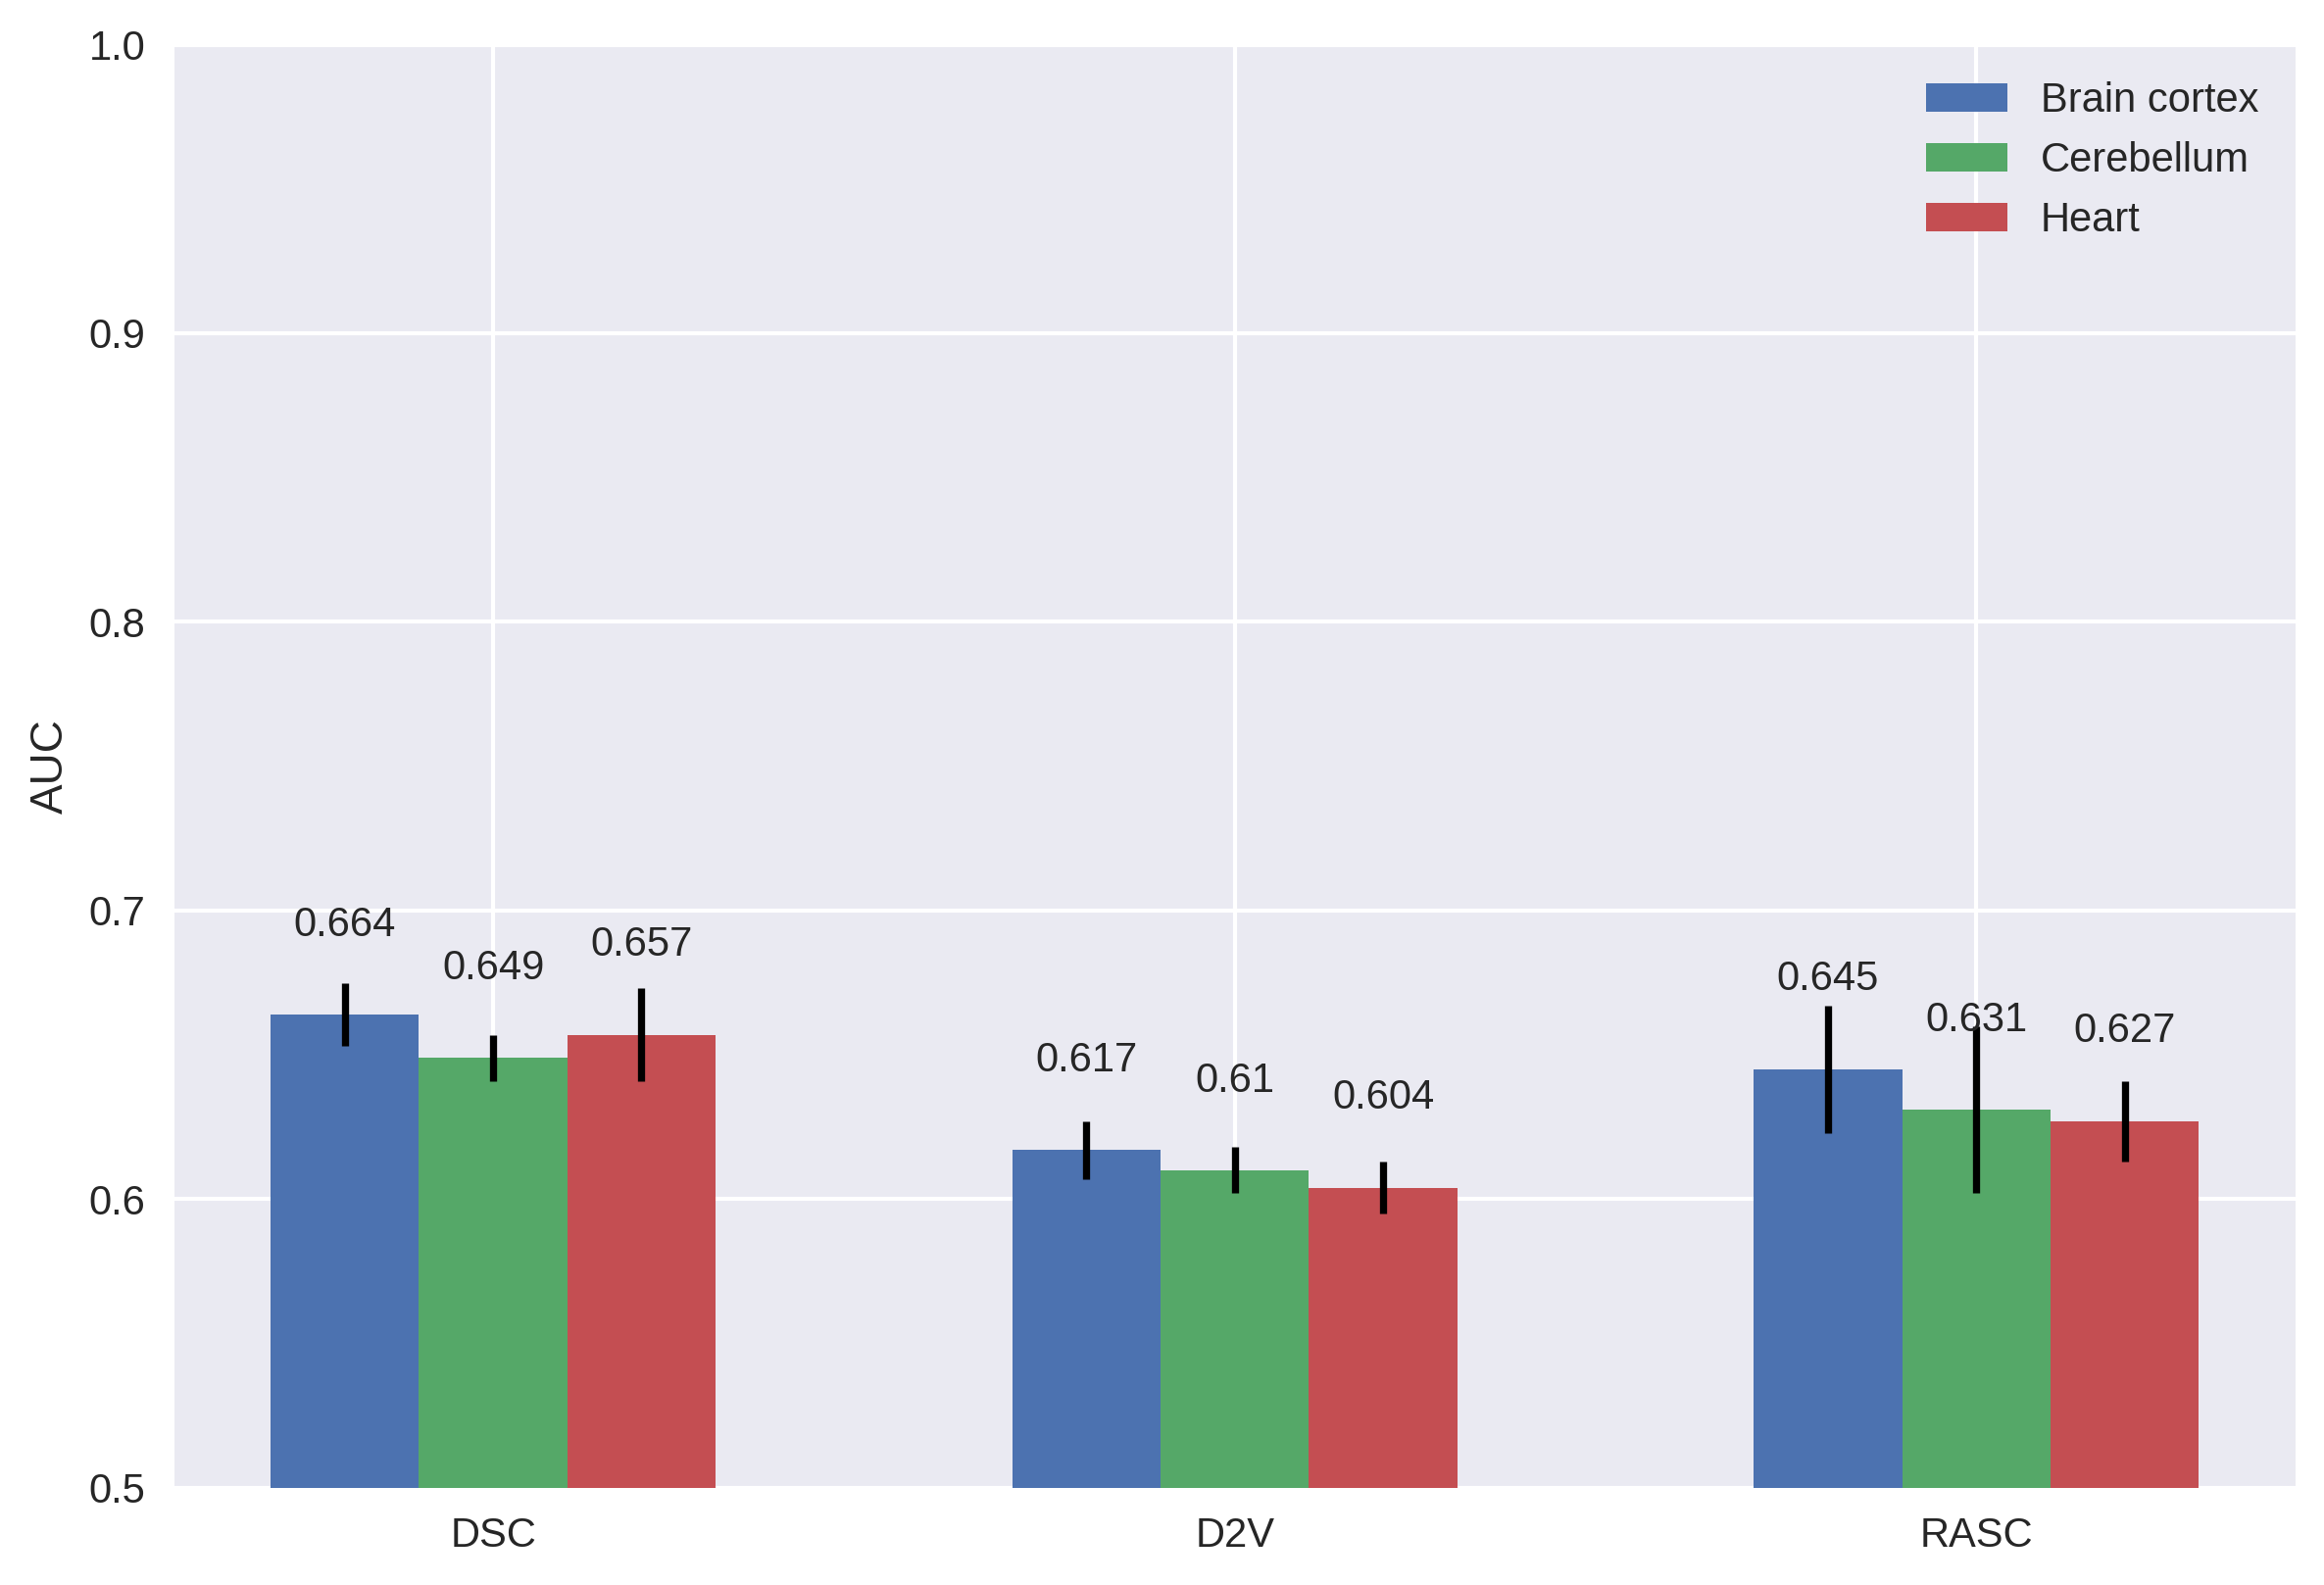
\includegraphics[width=0.85\textwidth]{../visualizations/ch5-results/gtex_exon_barcharts.png} 
	\caption{Performance on the GTEx-based exon-centric datasets across different tissues. The error bars give the standard deviation across all cross-validation runs. }
	\label{fig:gtex_exon_barcharts}
\end{figure}

\begin{figure}
%	\centering\includegraphics[width=0.7\textwidth]{../saved/log/GTEx_Exon_Brain_Attn/final/ROC.png} 
	\centering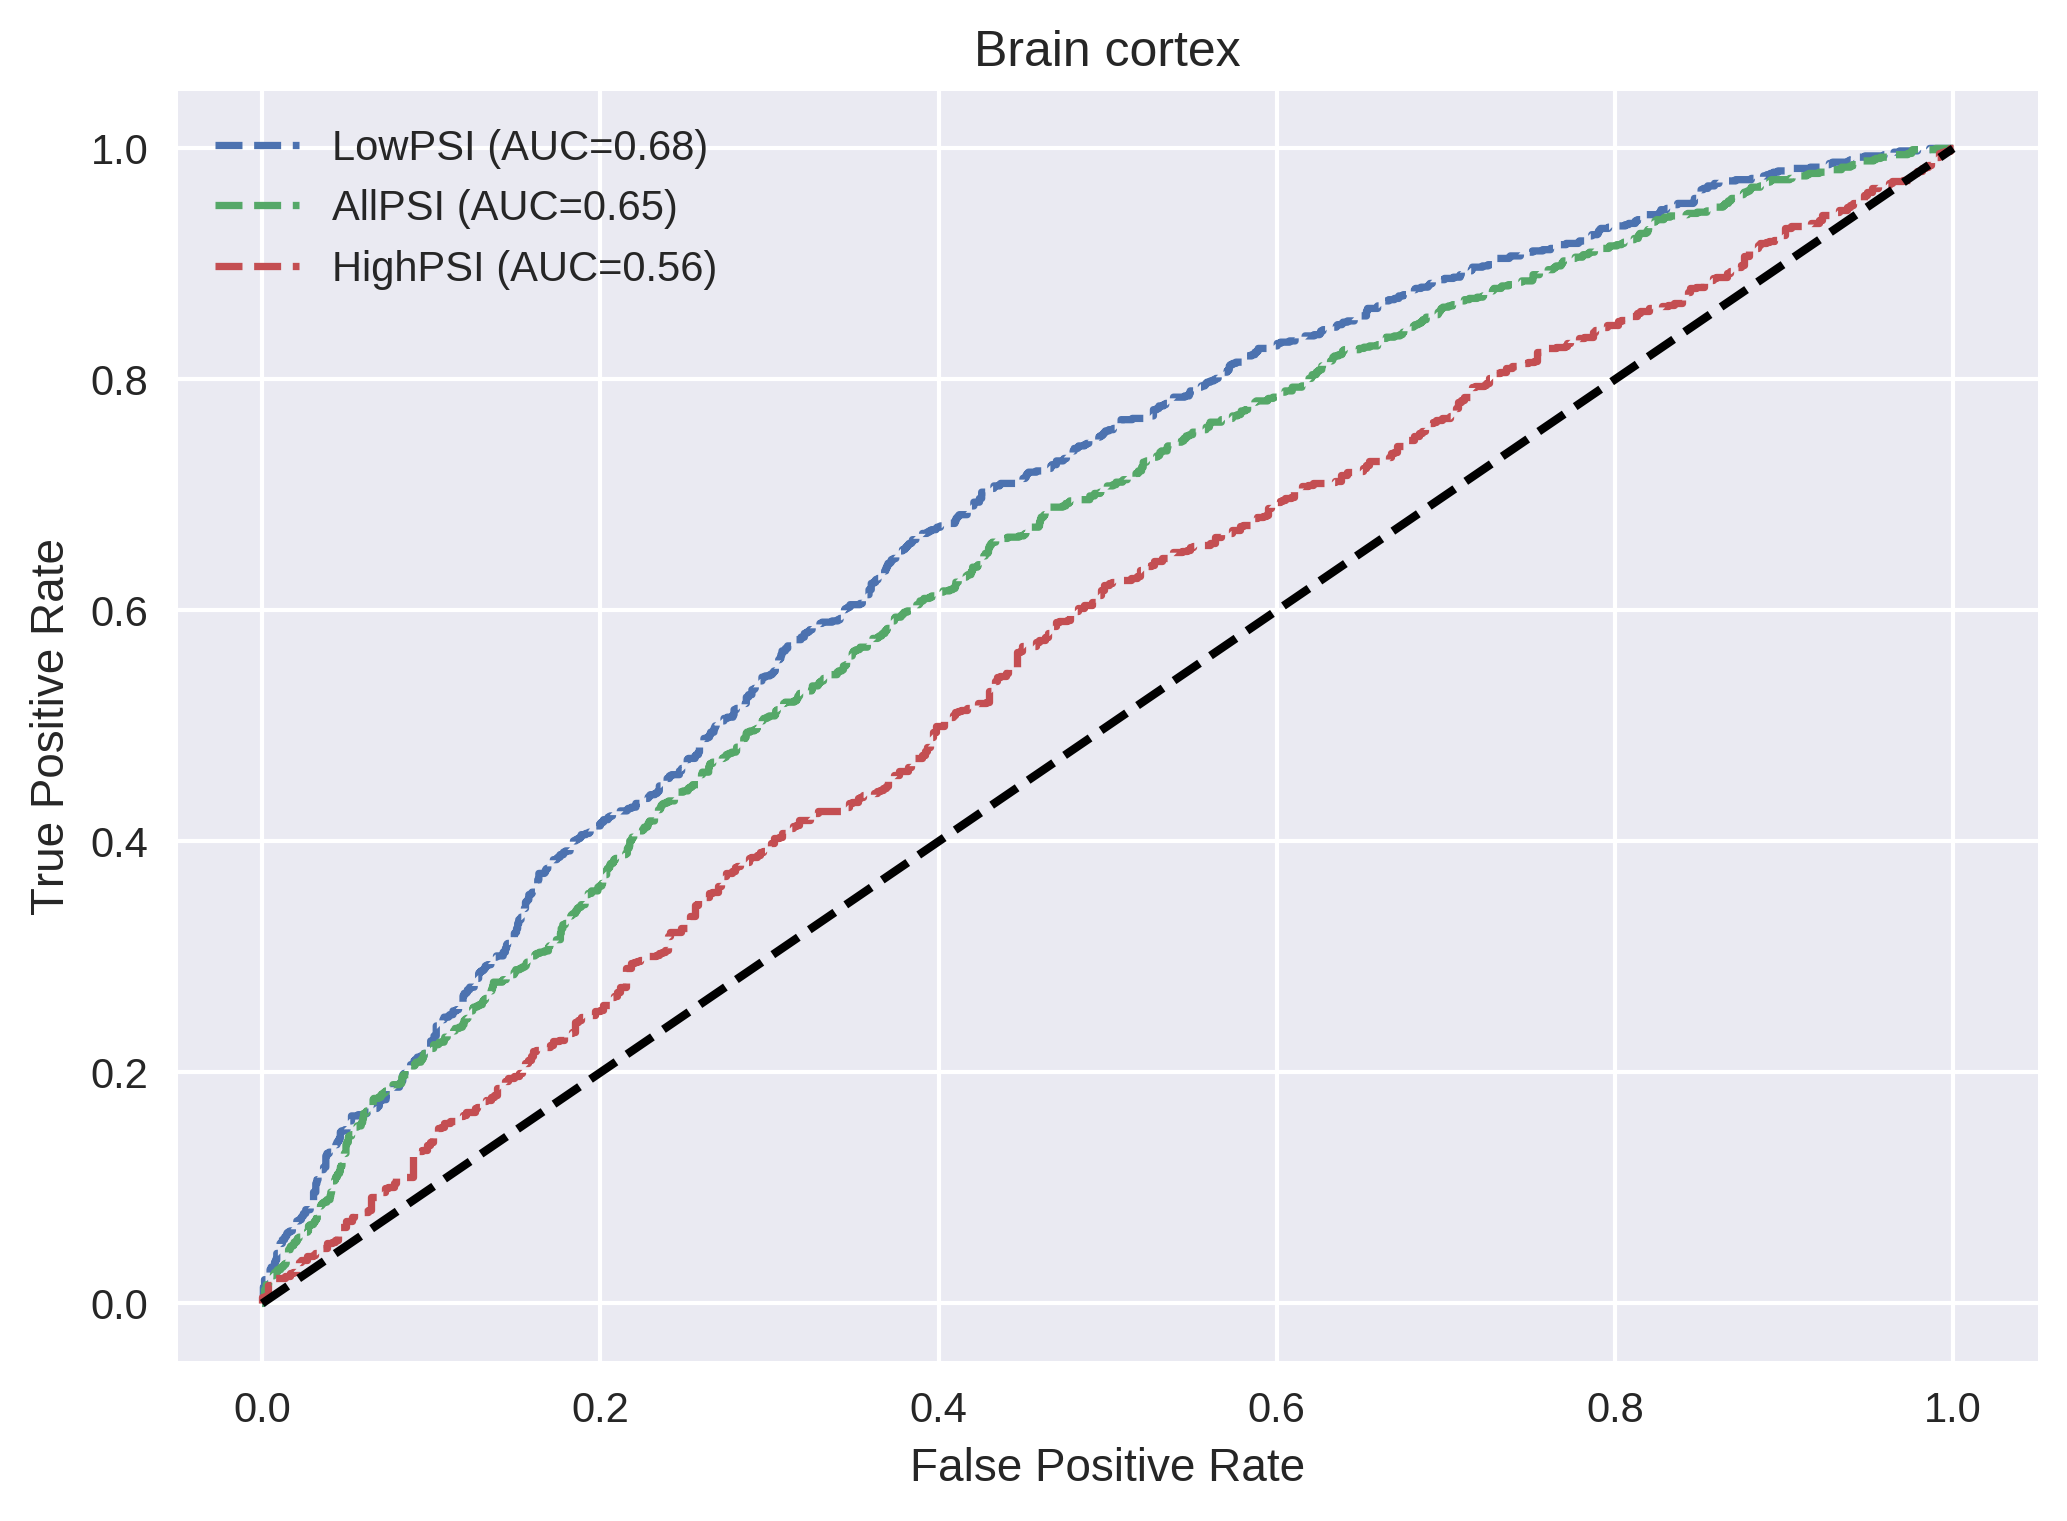
\includegraphics[width=0.7\textwidth]{../visualizations/ch5-results/gtex_exon_brain_roc.png} 
	\caption{
	ROC curve of RASC on GTEx-based exon-centric brain cortex dataset. 
  }
	\label{fig:gtex_exon_roc}
\end{figure}
\subsubsection{Main analysis}
Results are given in Figure \ref{fig:gtex_exon_barcharts}. Across all models, performance is poor: the highest mean performance we observe is 0.664 AUC. Surprisingly, performance is also very similar across tissues: the mean cross-tissue performance difference of 0.007 AUC is smaller than the mean cross-run difference of 0.014 AUC. This is surprising from a biological perspective as cross-tissue splicing differences are well-documented \cite{crosstissuesplicing}. 
This could indicate that, while splicing across tissues varies, the relative complexity of cassette exon splicing behaviour across the evaluated tissues is similar. However, this would be overinterpreting models with low predictive power.
Most likely, the models are already struggling to learn the baseline splicing behaviour invariant across tissues and don't learn finer cross-tissue differences. 
% that Since our models perform so poorly they likely already struggle to learn the baseline splicing behaviour invariant across tissues. 
The low cross-tissue performance differences also surprising from a machine learning perspective, as the cerebellum-based dataset contains almost twice as many training samples as the heart-based dataset. This indicates that either 1) the models have already hit a point of diminishing returns for adding more data or 2) the models generally require significantly more training samples. All models perform best on the dataset based on a brain cortex sample. 
%even if splicing varies across tissues, performance as measured by AUC could be the same if roughly same level of complexity -- avoid this issue by referrering to it as most likely explanation

Cross-model performance differences are small (mostly between 0.02-0.03 AUC), yet constant between tissues: DSC tends to perform best, followed by RASC and the D2V model. The variance of RASC between runs is on average twice as twice as high as the respective variance of DSC and D2V. As a result, RASC is the best performing model, as measured by the maximum rather than mean AUC value, on the brain cortex tissue-based and cerebellum tissue-based datasets. This indicates that RASC needed more regularization on this dataset and dataset specific fine-tuning could've lead to it performing the best across cross-validation runs.

\subsubsection{Differences between highly and rarely included exons}
Figure \ref{fig:gtex_exon_roc} gives more insight into model performance. 
The performance on highly included, alternatively spliced exons (80\% <= PSI < 99\%) is significantly worse than on more rarely included, alternatively spliced exons (PSI < 80\%). Per definition of the AUC, the AUC on the allPSI dataset lies in-between these two extremes. In this case, only $\sim$28\% of alternatively spliced exons belong to the exons with a high PSI and therefore the combined AUC is heavily weighted towards the AUC on the exons with low PSI. These observations mirror analogue observations made on the HEXEvent dataset \cite{dsc}.

%---- removing length feature would be interesting; doing it on brain as best performance and sort of lowest combined variance\\


%- could note that in earlier variation of the dataset where no TPM treshold was used (?) the networks didn't learn anything\\
%	-- would be great finding out / remembering what exact step is the crucial one
%	




%\textbf{conclusions:}\\
%	- performance generally poor\\
%	- inter-tissue variance low\\
%	- due to issues with GTEx data, likely desirable to test with other datasets
	
	
	

\subsection{Intron-centric datasets} \label{subsec:gtex_junc}

\begin{figure}[h]
	\centering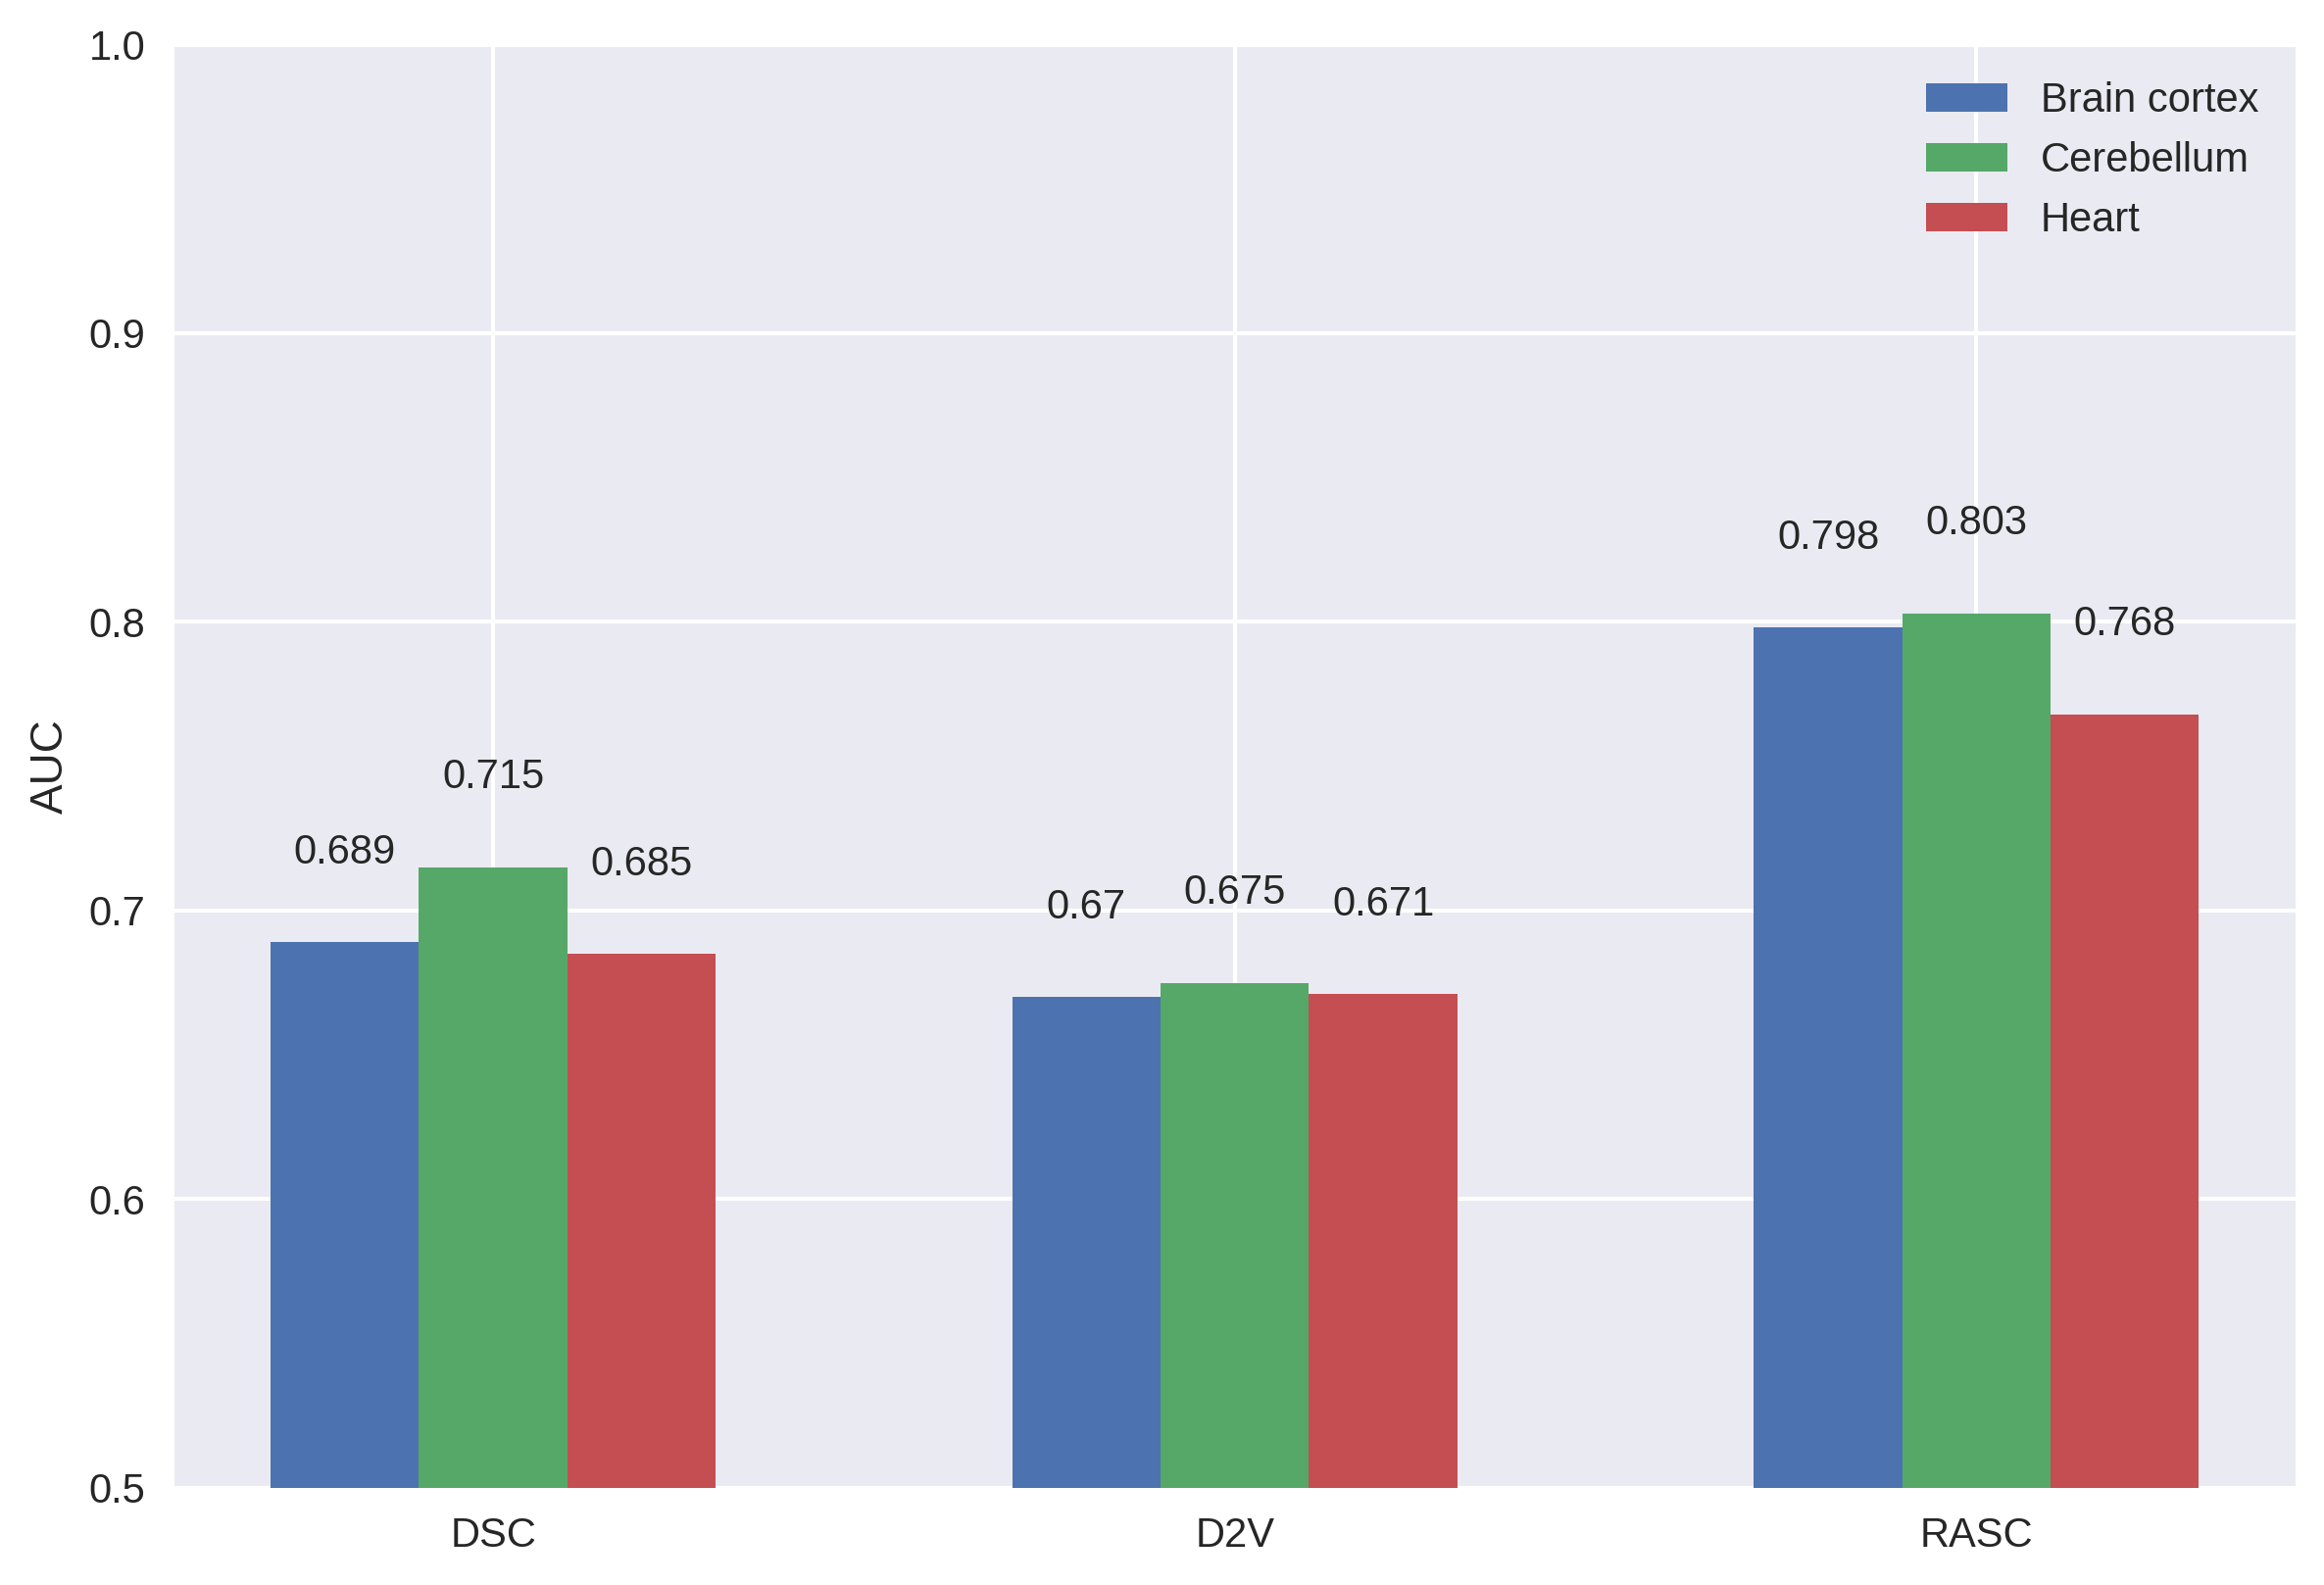
\includegraphics[width=1\textwidth]{../visualizations/ch5-results/gtex_junc_barcharts.png} 
	\caption{Performance on the GTEx-based junction datasets across different tissues. }
	\label{fig:gtex_junc_barcharts}

\end{figure}


\begin{figure}[h]
%	\includegraphics[width=0.5\textwidth]{../saved/log/GTEx_Junc_Heart_DSC/final/ROC.png} 
%	\includegraphics[width=0.7\textwidth]{../saved/log/GTEx_Junc_Heart_Attn/junc_cv_final/ROC.png}
	\centering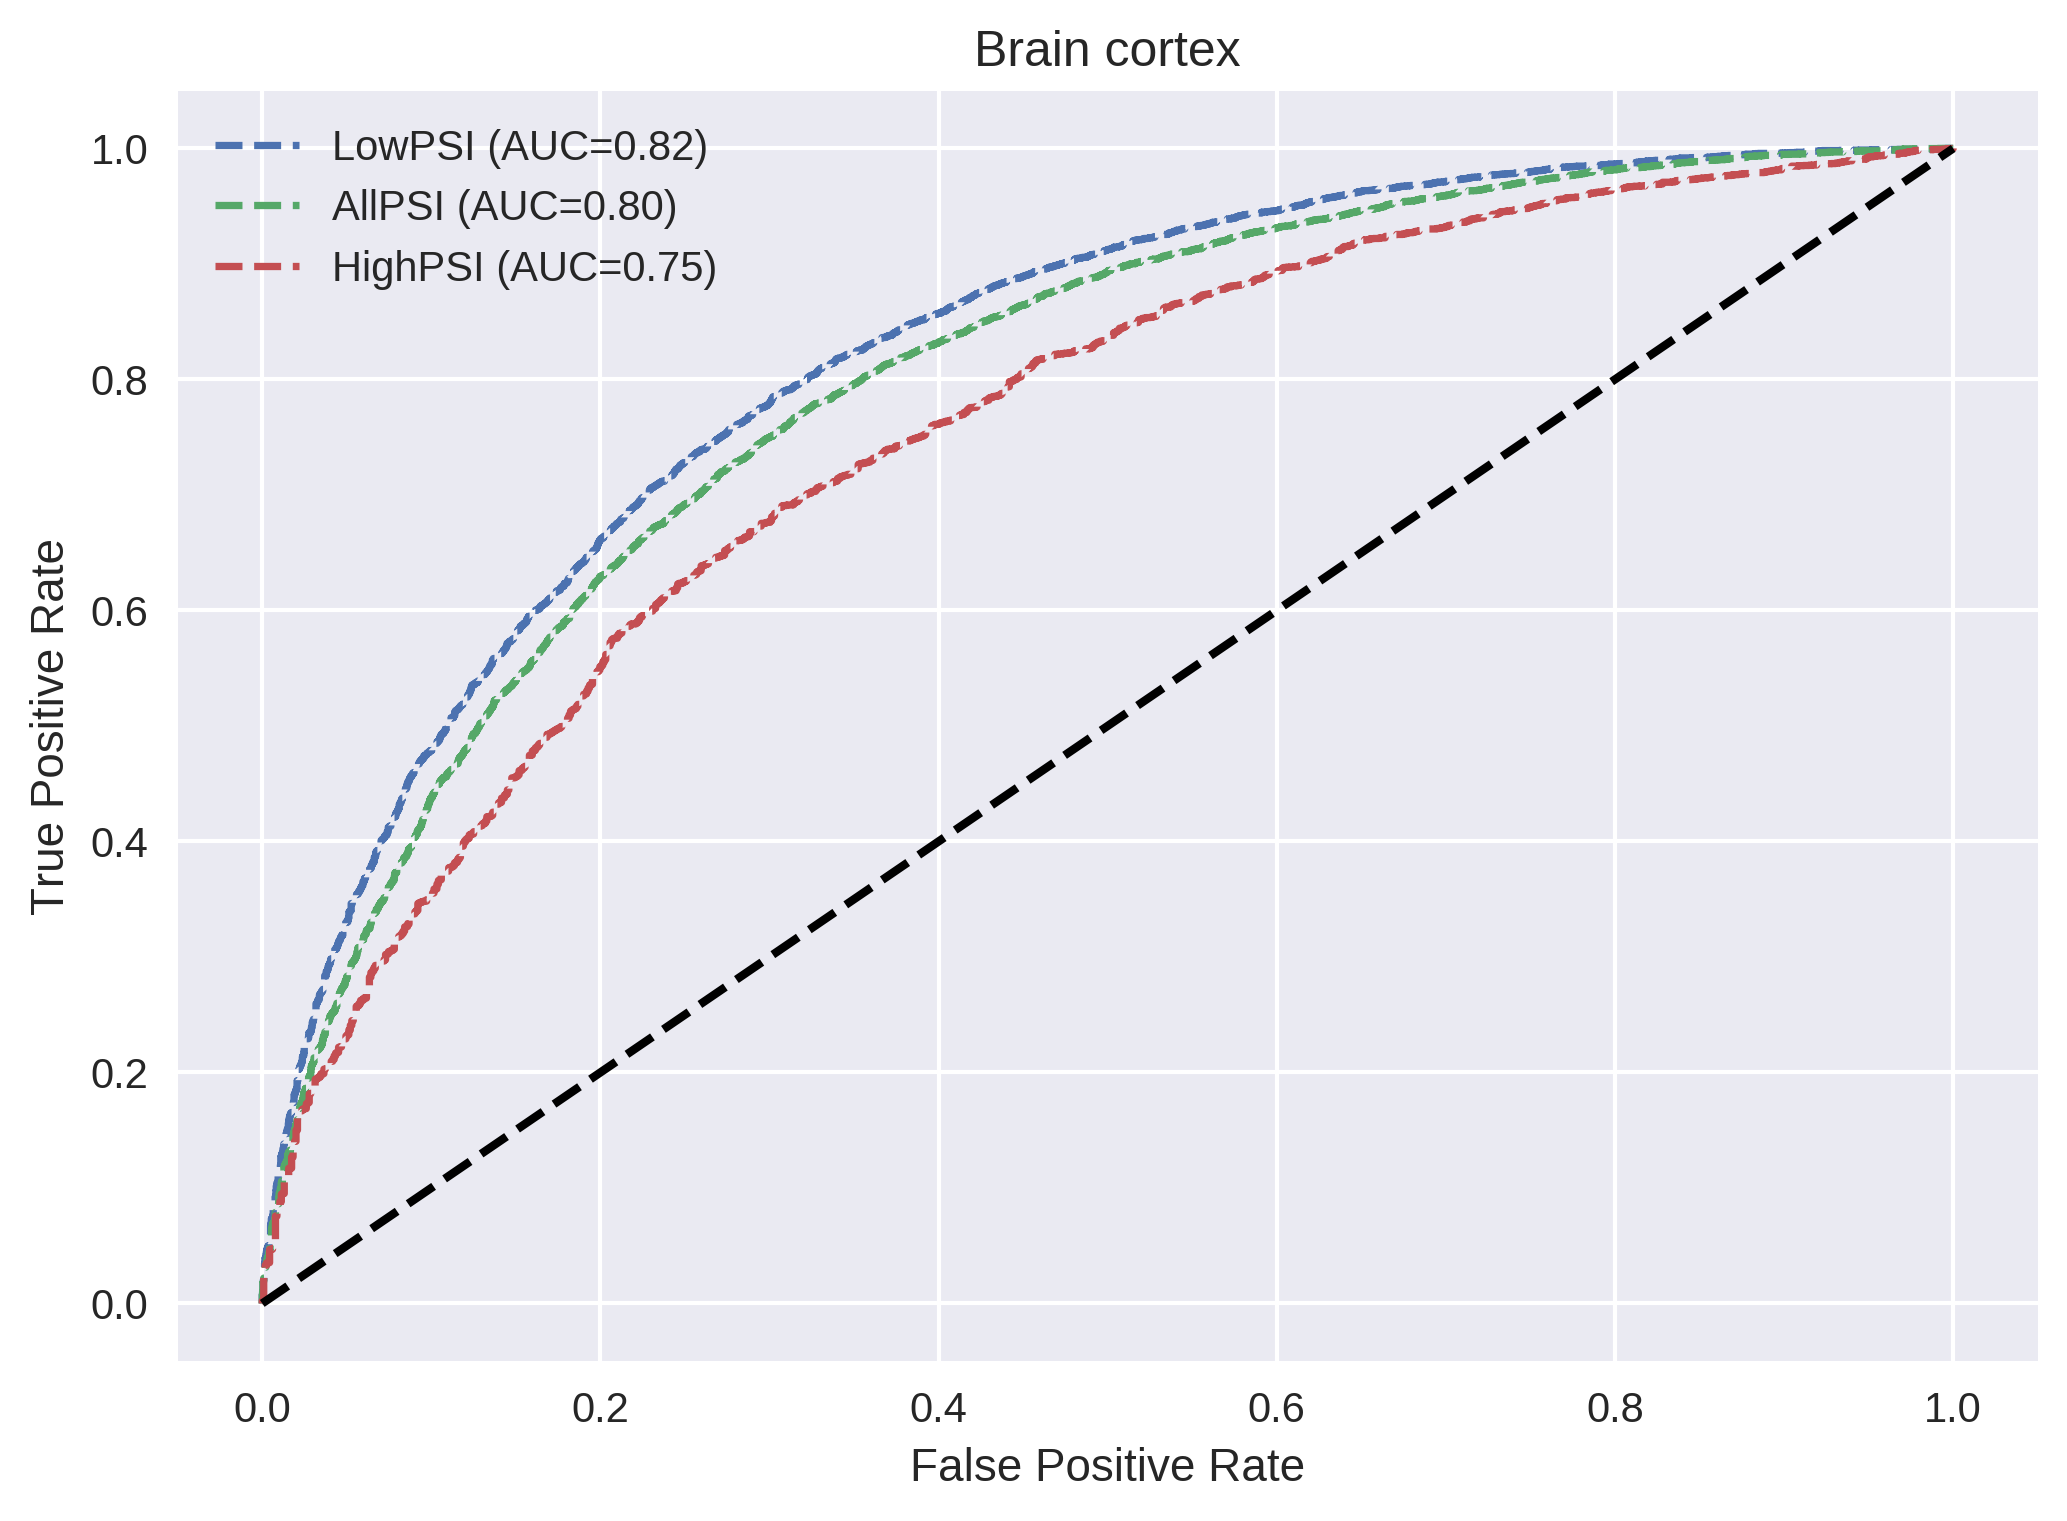
\includegraphics[width=0.7\textwidth]{../visualizations/ch5-results/gtex_junc_brain_roc.png} 
	\caption{ROC curve from training RASC on the GTEx-based intron-centric brain-cortex-tissue-based dataset. }
	\label{fig:gtex_junc_rocs}
\end{figure}



\subsubsection{Main analysis}
Figure \ref{fig:gtex_junc_barcharts} shows that the AUC of all models increases by at least 0.05 to 0.06 compared to the exon classification task. This is likely a result of the intron-centric datasets containing on average four times more training samples than the exon-centric datasets. The performance of RASC is the most promising and experiences the largest growth (by 0.15 AUC) demonstrating its capacity to capitalize on the increased number of training samples. The corresponding classification accuracy of RASC, when choosing the decision threshold which maximizes the F1 score, is roughly 70\% and shows that there is still room for further improvement. 

Similar to the exon-centric datasets \ref{subsec:gtex_exon}, we observe very low cross-tissue performance differences. We again believe that model performance is generally too poor to warrant speculation about the underlying biological realities. However, we come to a different conclusion regarding the observation that the different dataset sizes between tissues don't affect model performance:
for the GTEx-based exon-centric datasets we hypothesized that the models have hit diminishing returns for adding more data or that they need significantly more data. As the number of training samples has quadrupled in the move from exon- to intron-centric datasets, we now believe that the models have hit a point of diminishing returns for adding more data. 



The performance across rarely and highly included junctions is less disparate than on the exon-centric datasets (see Figure \ref{fig:gtex_junc_rocs}). This indicates that the models are better able to learn to recognize motifs which separate constitutive and highly alternatively spliced junctions than for exons.
%However, this observation may not be very epistemiologically certain as only 15\%
% explanation for this

\subsubsection{Assessing model performance without length features}

\begin{table}[h!]
	\centering
	\resizebox{\textwidth}{!}{\begin{tabular}{| l | c | c | c| c} 
		\hline
		Model name & Only sequences & Sequences + lengths & Relative gain\\
		\hline
		DSC & 0.661 & 0.704 & 0.211\\
		D2V & 0.629 & 0.673 & 0.254\\
		RASC & \textbf{0.776} & \textbf{0.808} & 0.104\\
		\hline
	\end{tabular}}
	\caption{Performance on the GTEx-based intron-centric dataset with and without length features. 
		%		Note that the relative performance drop was computed with reference to the baseline AUC value of 0.5.
	}
	\label{table:gtex_junc_nolens}
\end{table}

As model performance is more promising than on the GTEx-based exon-centric datasets, we validate that this isn't due to an overreliance on the length features as on the HEXEvent dataset. Table \ref{table:gtex_junc_nolens} shows that the length features still make up a large part of model performance, but that the models don't rely on them completely. However, the performance proportion the length features account for is still biologically implausible. 

Thus we conclude that the dataset is an improvement over the HEXEvent dataset, but generating a dataset where model performance is less dependent on the length features is still desirable. 


%15 \% of alternatively spliced exons are highly included 

%\subsection{Reconstructing HEXEvent-dataset with GTEx data}
%- dataset where I only took exons which were also in GTEx data\\
%- seriously considering not showing these results as I basically already debunked HEXEvent at this point -- so from a narrative perspective, why spend effort on replicating it?

\subsubsection{Evaluation of the GTEx-based datasets}
Overall, we observe poor to promising model performance, biologically surprising low cross-tissue performance differences and biologically implausible reliance on the length features. 
In \ref{subsubsec:naivepsi}, we mentioned issues when trying to estimate PSI naively. Although we alleviated these in pre-processing, we don't account for the information contained in non-junction reads and don't integrate information from multiple samples. As a result, data quality is likely still an issue distorting the results in this section. 
Thus we conclude that the GTEx-based datasets improve upon the HEXEvent dataset, but using datasets based on more accurate PSI estimation methods is desirable and would lead to more meaningful results. %would lead to more meaningful results.

%Alleviating these issues, we next evaluate the models based on a primary data source which gives access to raw RNA-seq reads. This enables us to use methods from the literature which leverage information from non-junction reads and multiple samples.

%Overall, we observe poor model performance and biologically surprising low cross-tissue performance differences. This indicates that the GTEx-based exon-centric dataset is not fit for training neural-network based splicing codes and conclude that evaluating the models on other datasets is desirable.



\section{HipSci SUPPA datasets} \label{subsec:hipsci_suppa}
\subsection{Dataset based on iPSC-derived sensory neuron cell lines}

\begin{figure}
	\centering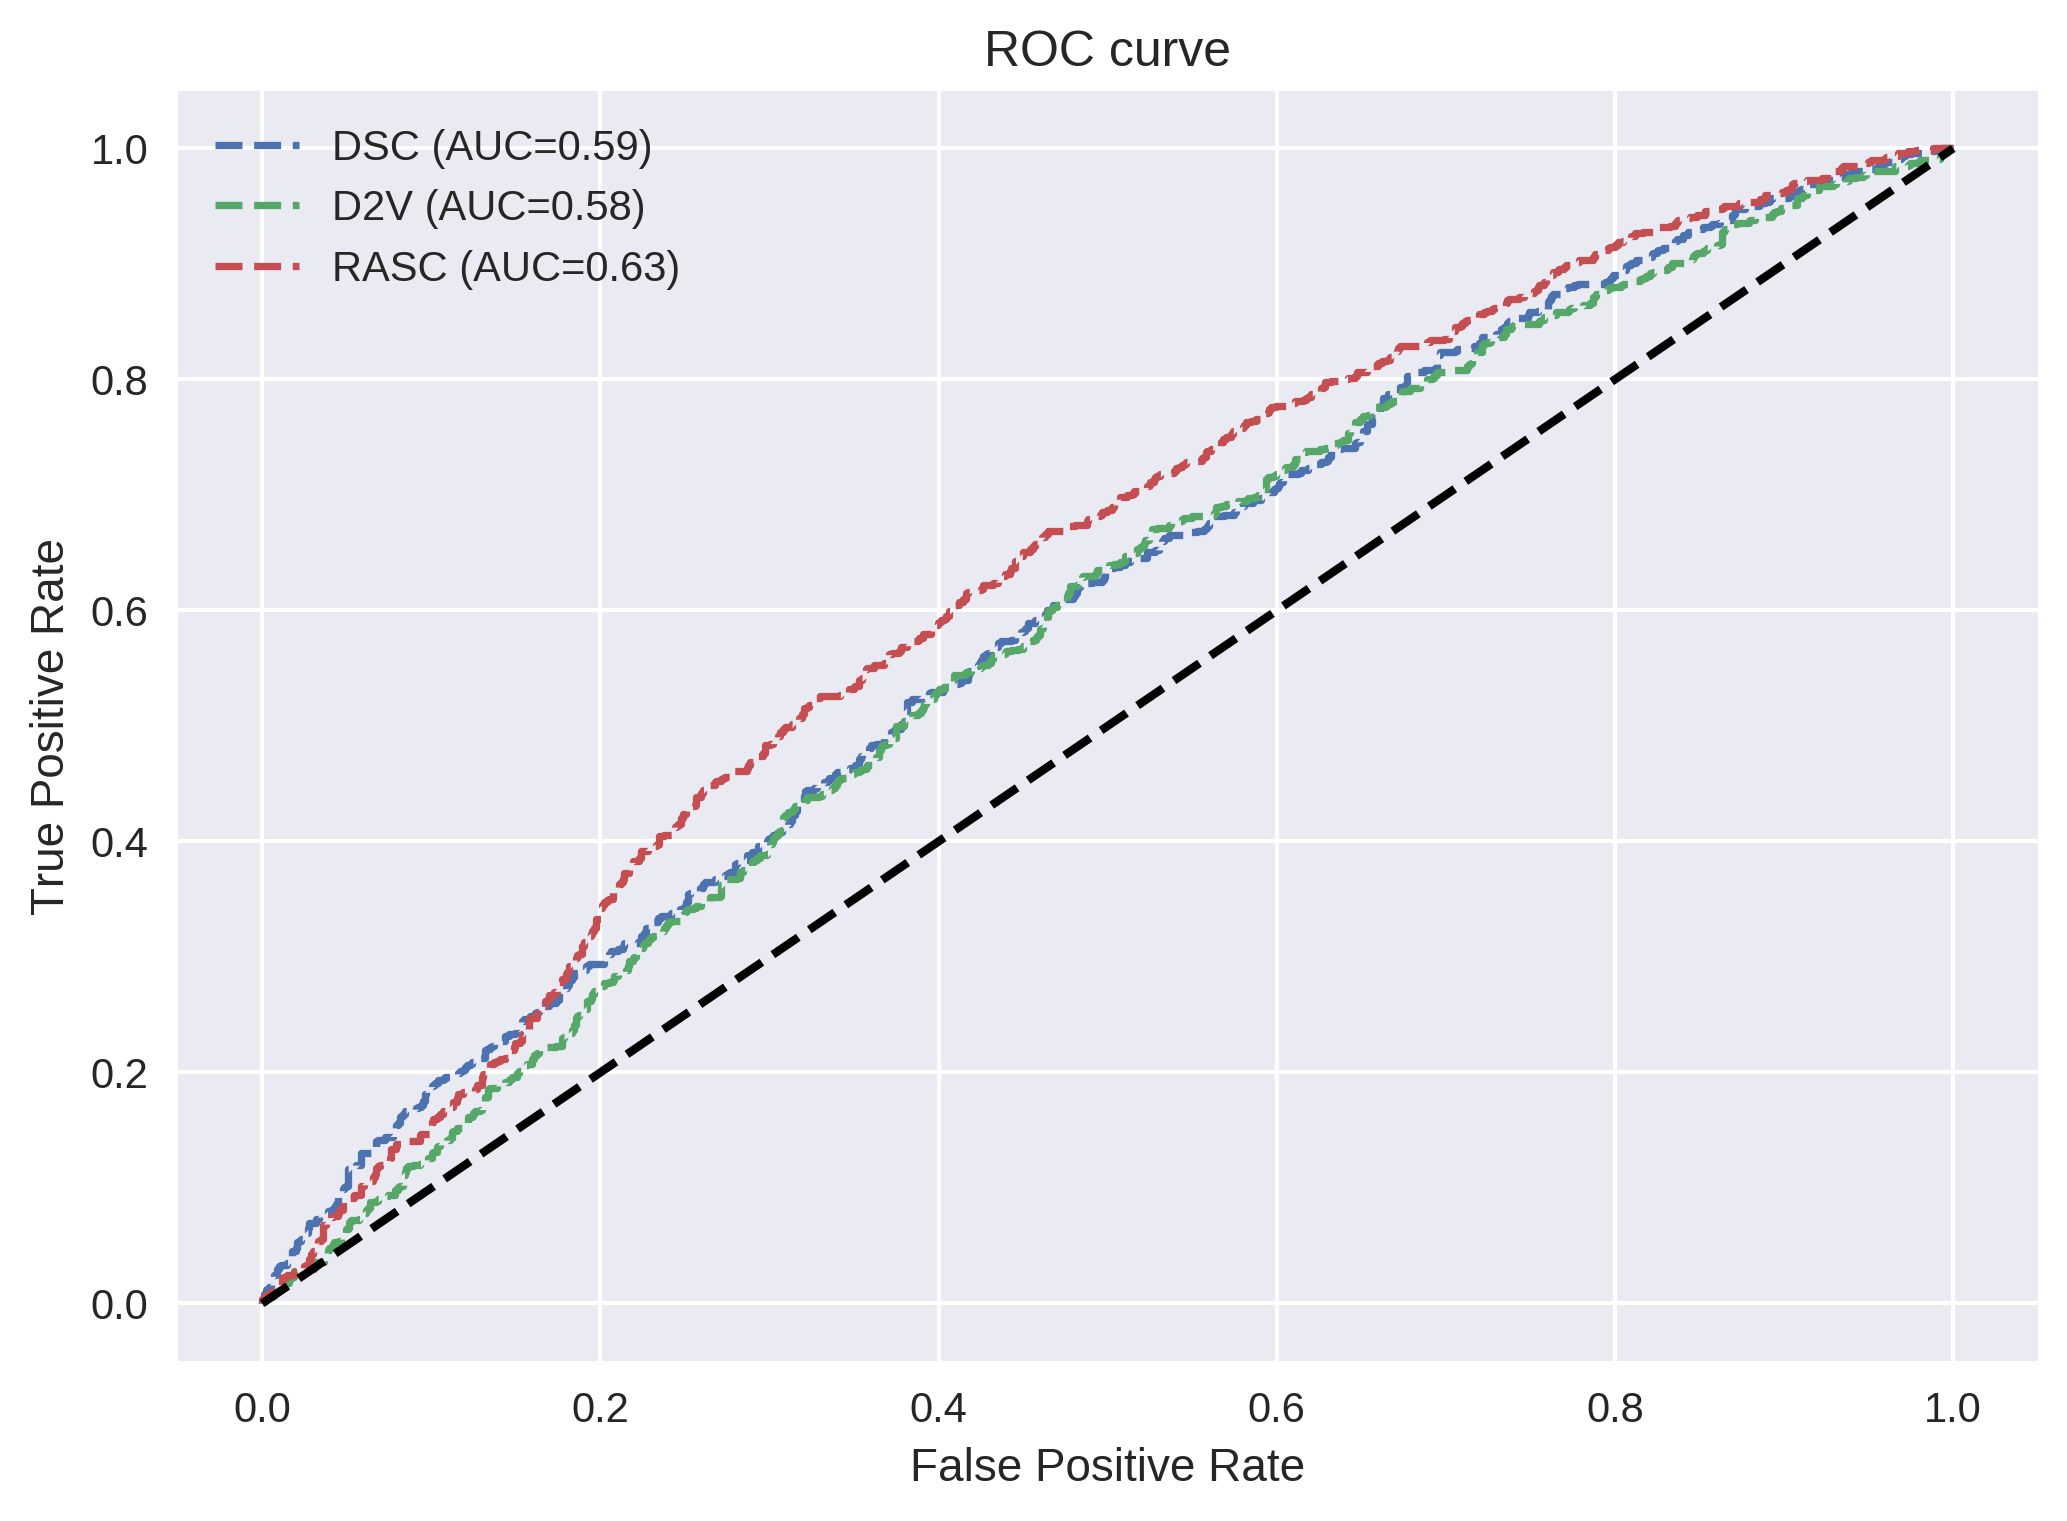
\includegraphics[width=0.7\textwidth]{../visualizations/ch5-results/suppa_cross_model_roc_auc_comparison.png} 
	\caption{Comparison of the ROC curves of the three models on the HipSci SUPPA dataset. The dataset is based on iPSC lines differentiated to sensory neuron cell lines. }
	\label{fig:suppa_auc_roc}
\end{figure}
\subsubsection{Main analysis}
Figure \ref{fig:suppa_auc_roc} shows how the model perform very poorly on the HipSci SUPPA dataset. The performance is worse than on the GTEx-based exon-centric dataset and roughly equal to the performance on the HEXEvent dataset without length features. This indicates that 
\begin{enumerate}
	\item either we arrive at a strong dataset here and that constitutive exon classification is more challenging than so far anticipated,
	\item or this dataset suffers from data quality and quantity issues which make constitutive exon classification very challenging for the models.
\end{enumerate}

Among these two, 2. is more likely because SUPPA does not address various challenges in PSI estimation and because it does not generate constitutive training samples (see also \ref{subsubsec:suppa}). SUPPA does not appear to be suited for our purposes. Therefore, we skip the evaluation of the models on the HipSci SUPPA dataset based on undifferentiated iPSC lines.


%in retrorespect, SUPPA was not the best choice for dataset processing. It operates at a transcript level and therefore implicitly relies on the assumption that all transcripts of a given gene are known - this is often not the case. Additionally, it does not make it possible to generate a list of non-cassette constitutive exons, therefore roughly halving the size of the training set and the number of samples the model can learn from. Its PSI estimation is very simplistic and doesn't account for multiple of the issues highlighted in \ref{subsec:psiestimation}. Thus, we now turn to data processing with MAJIQ in hopes of better results. 

%thought: what if AUC here is only worse because the model doesn't have easy to classify constitutive exons which boost the AUC? 


\section{HipSci MAJIQ datasets} \label{subsec:majiq}

\subsection{Dataset based on sensory neuron cells and iPSCs}\label{sec:hipsci_neuron_majiq}

%\begin{figure}
%	\centering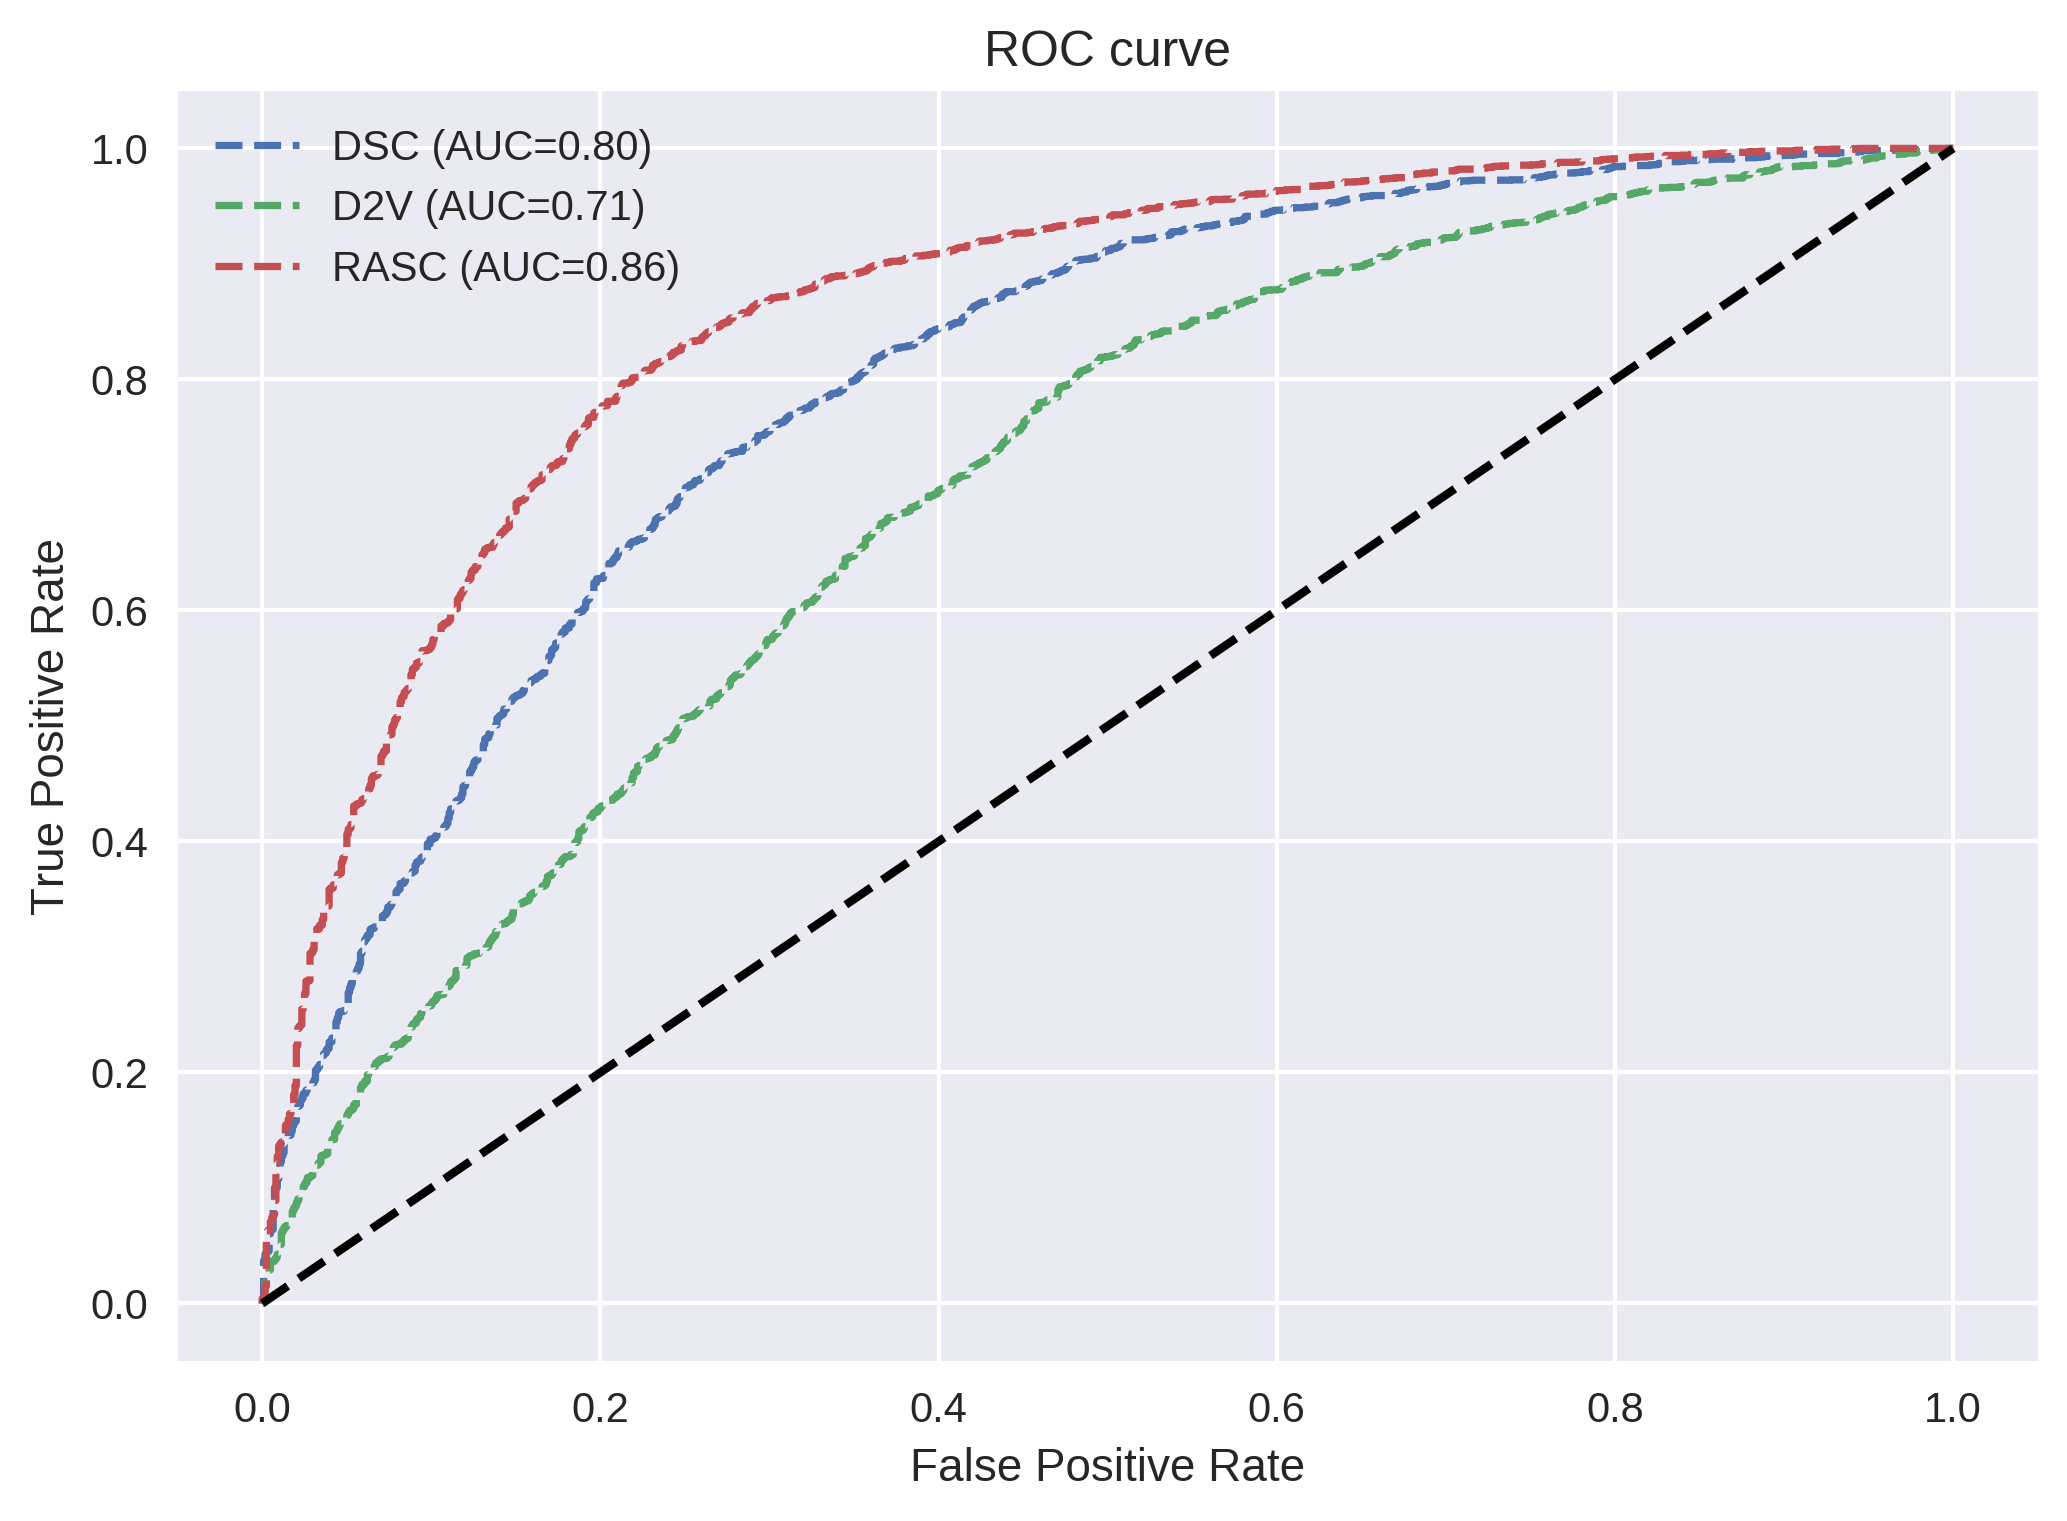
\includegraphics[width=0.49\textwidth]{../visualizations/ch5-results/majiq_neuron_cross_model_roc_auc_comparison.png} 
%	\centering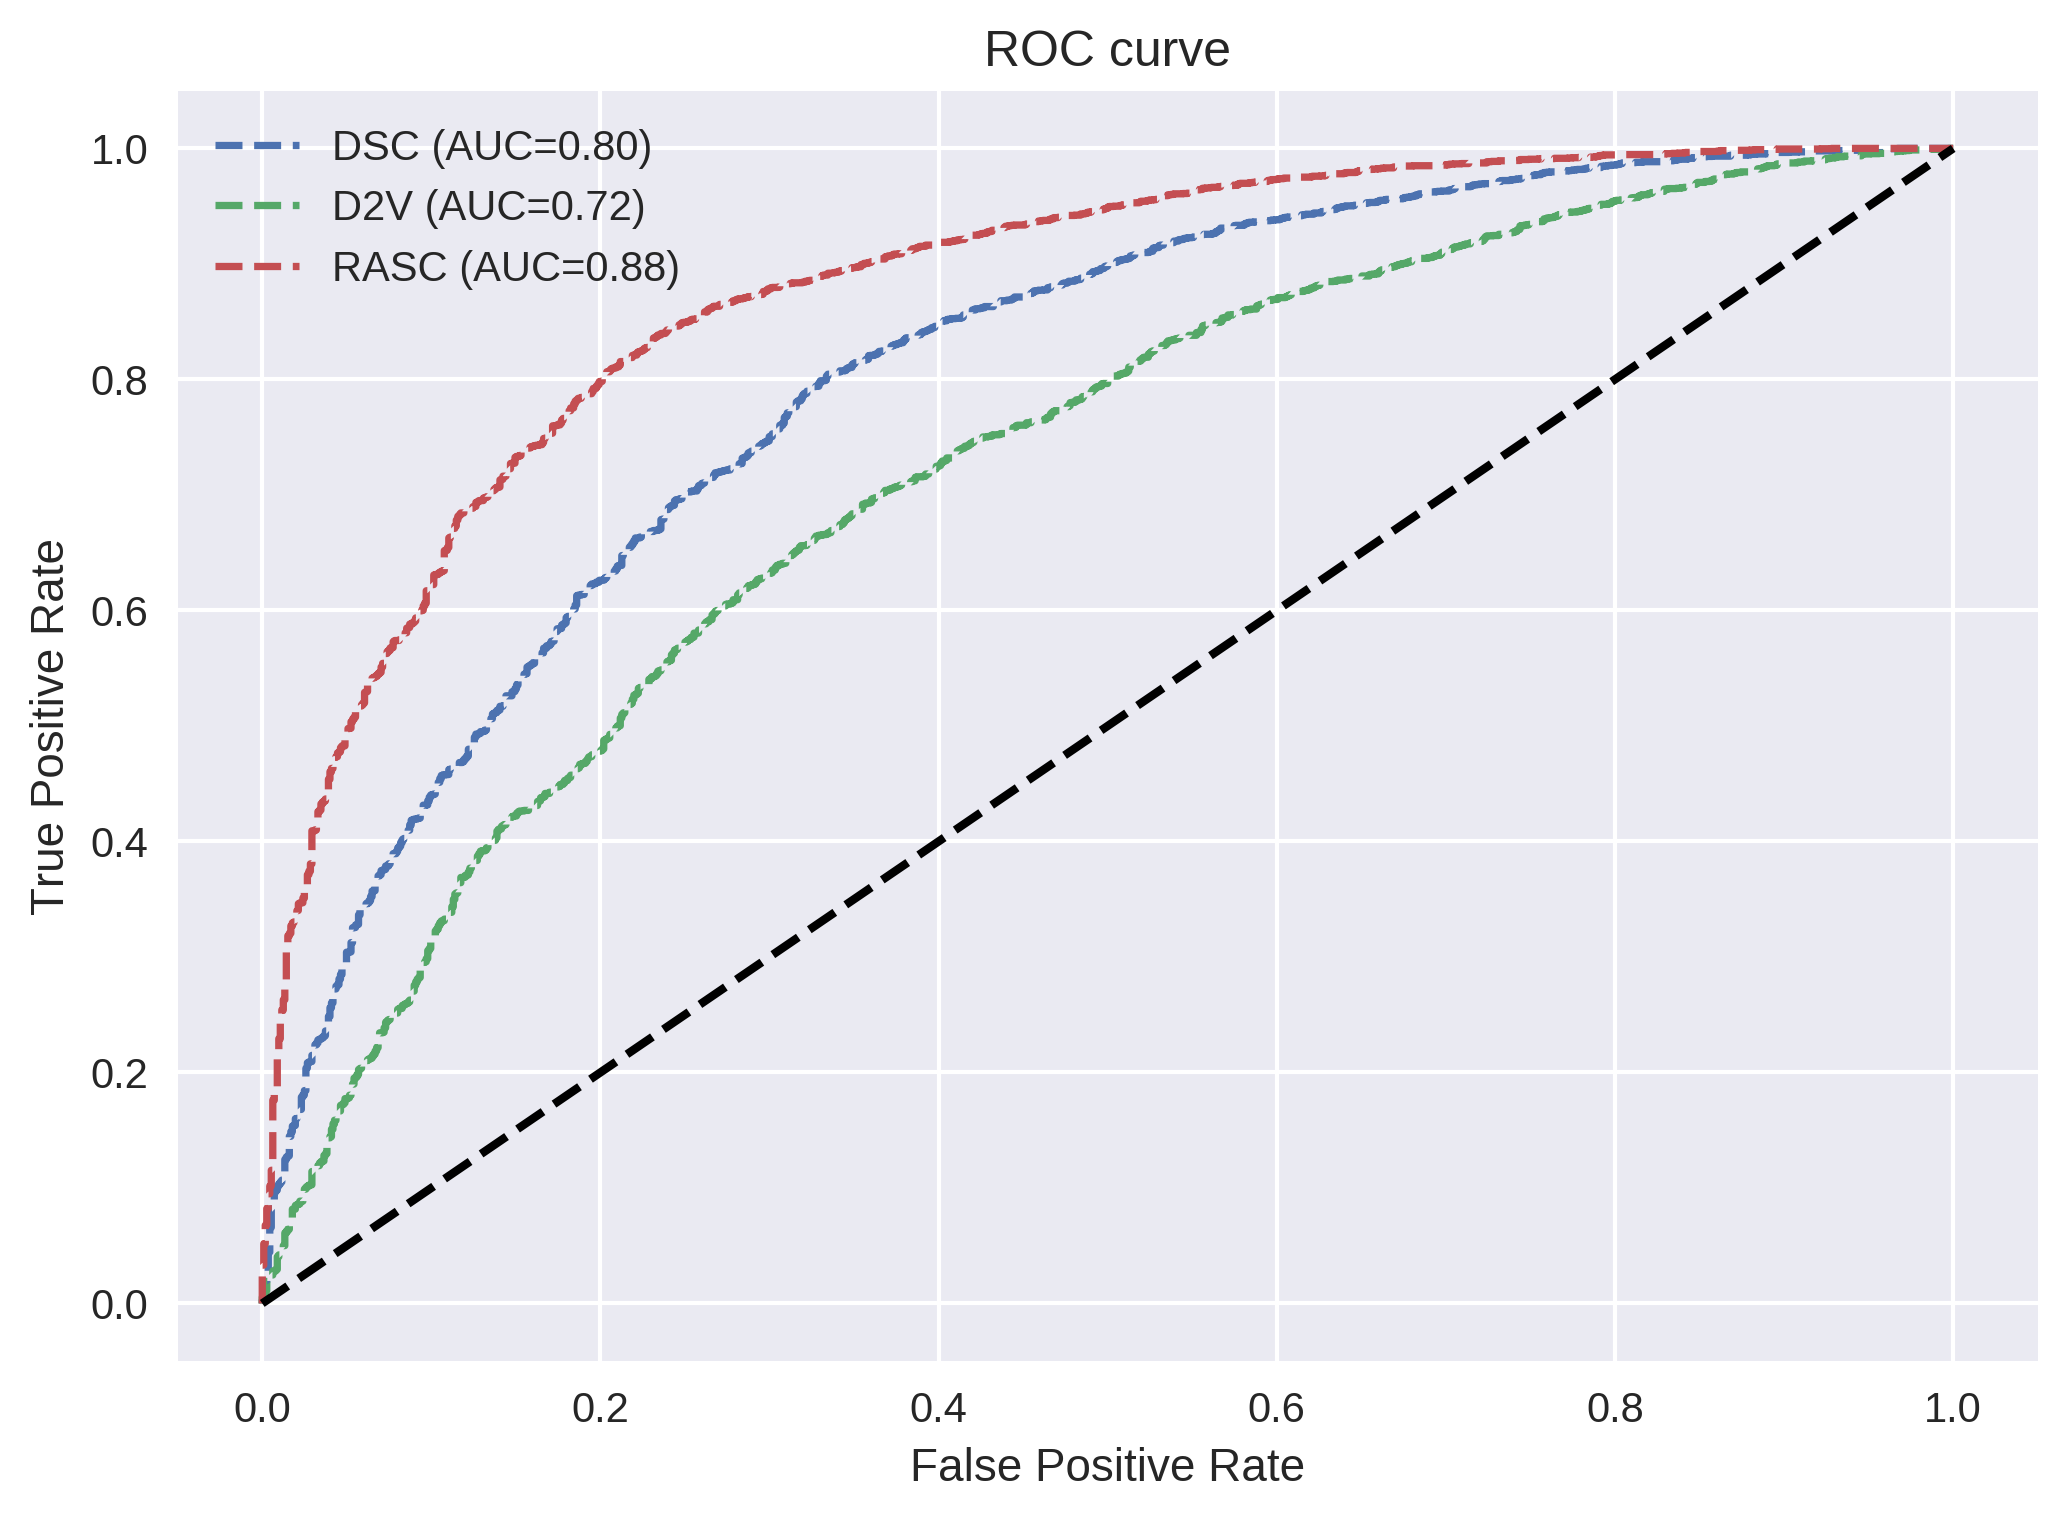
\includegraphics[width=0.5\textwidth]{../visualizations/ch5-results/majiq_ipsc_cross_model_roc_auc_comparison.png} 
%	\caption{Left: ROC curves on dataset based on processing with MAJIQ and iPSCs differentiated to neurons. Right: ROC curves on dataset based on processing with MAJIQ and undifferentiated iPSCs. }
%	\label{fig:majiq_rocs}
%\end{figure}



\begin{figure}
	\centering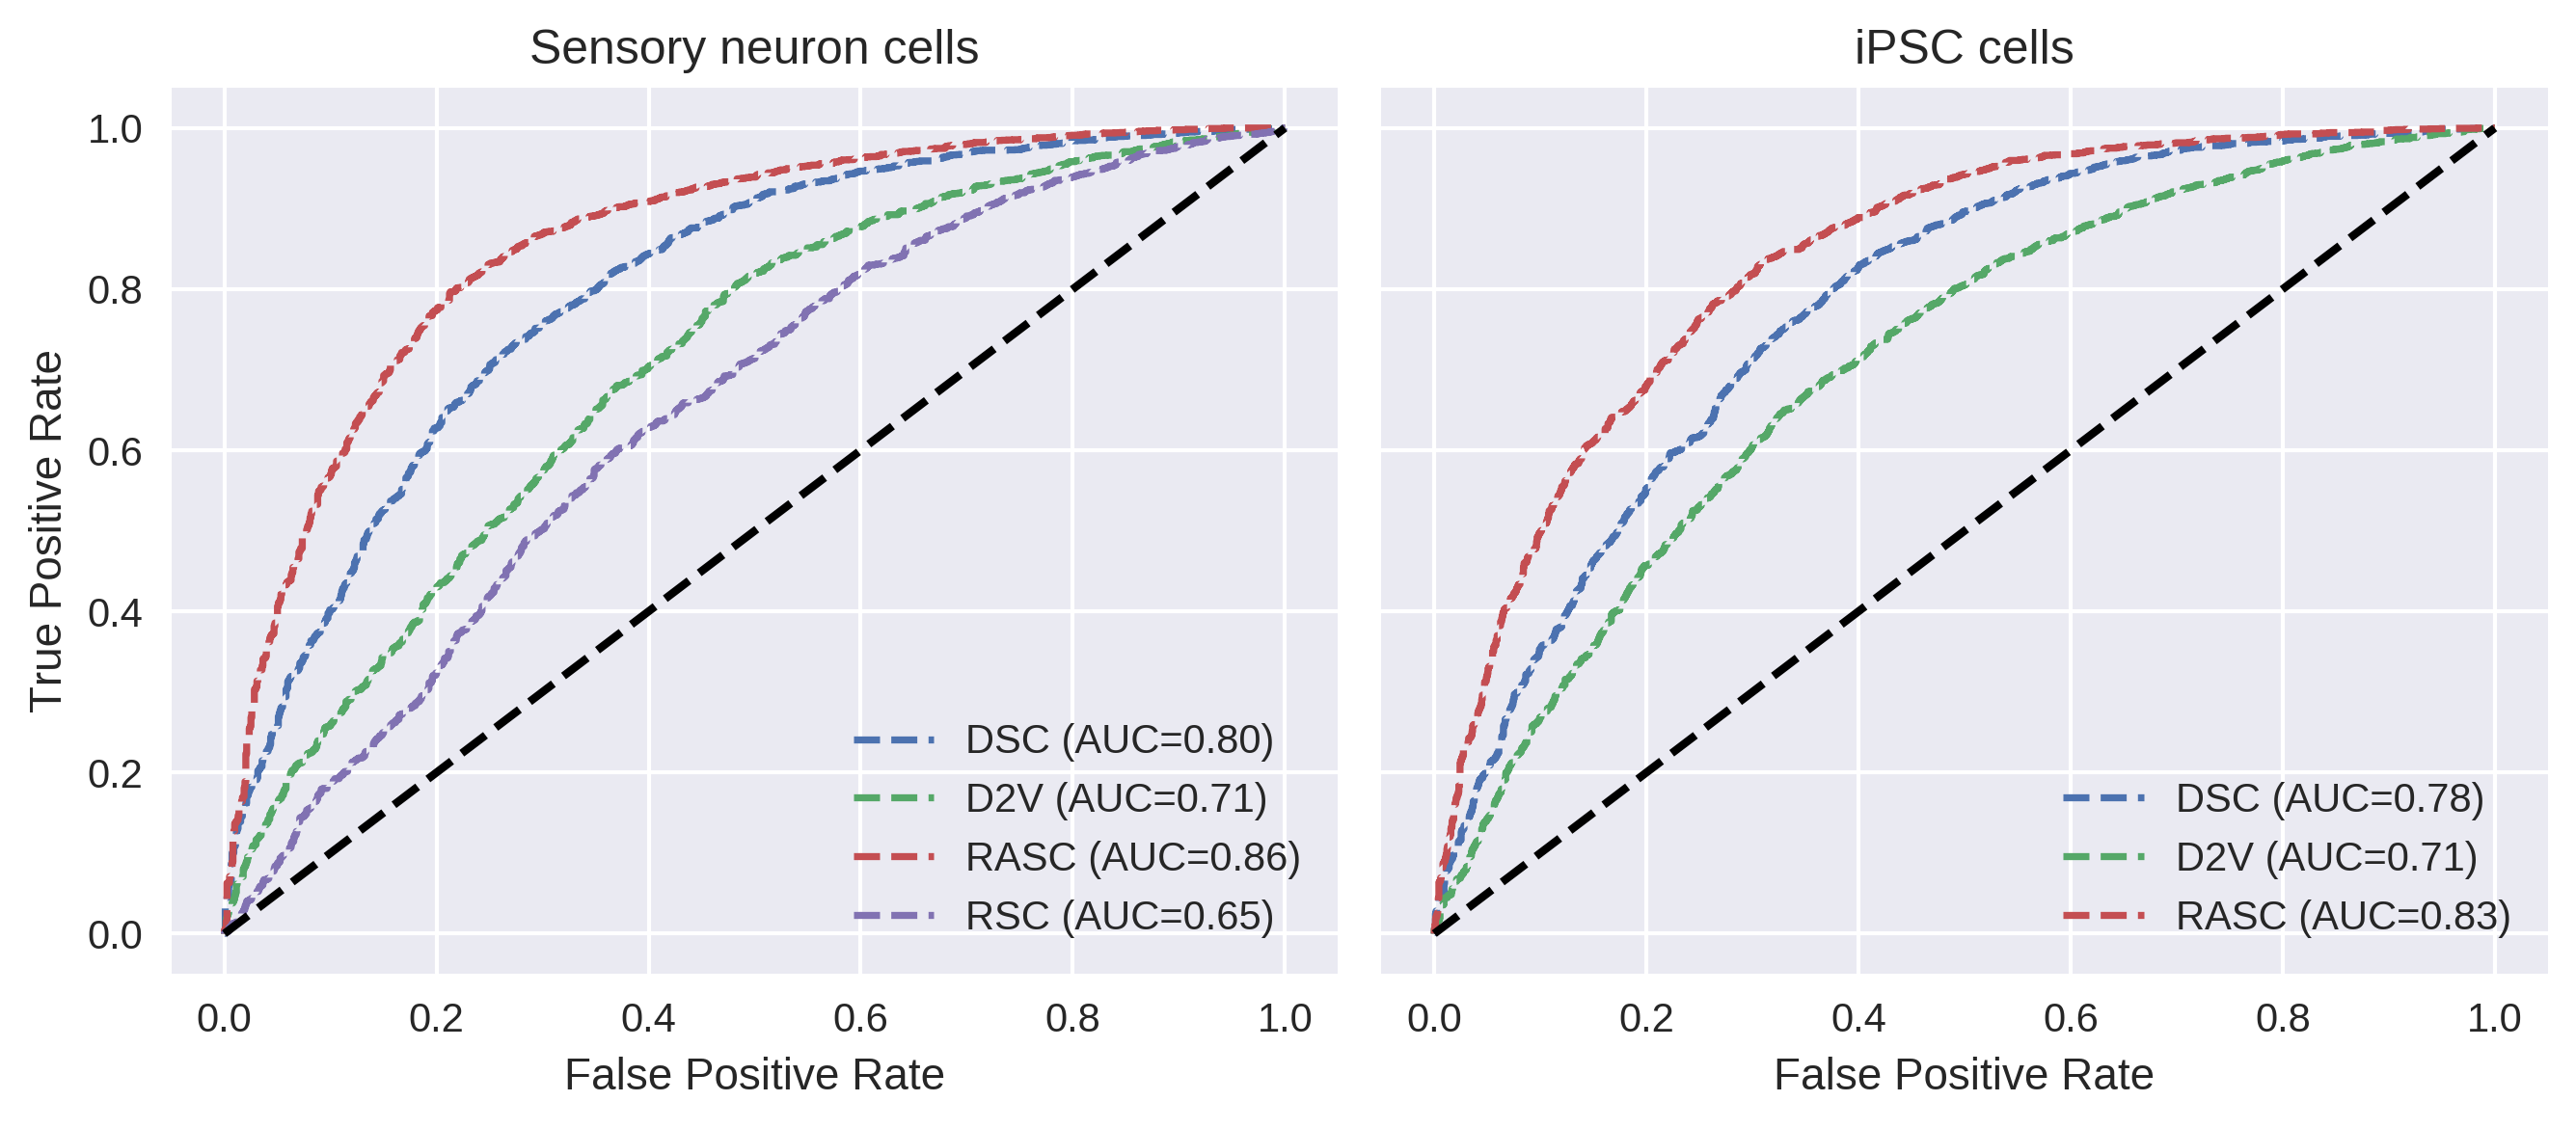
\includegraphics[width=1\textwidth]{../visualizations/ch5-results/majiq_neuron_ipsc_cross_model_roc_auc_comparison.png} 
	\caption{Left: ROC curves on HipSCi MAJIQ dataset derived from iPSCs differentiated to neurons. Right: ROC curves on HipSCi MAJIQ dataset derived from undifferentiated iPSCs. }
	\label{fig:majiq_rocs}
\end{figure}

\subsubsection{Main analysis}
All models perform significantly better than on previous datasets and we observe stark disparities between the models (see Figure \ref{fig:majiq_rocs}). While DSC outperforms D2V by a significant margin, it is outperformed by a similar margin by RASC. Adding attention to RSC promotes it from the worst to the best performing model, validating our choice. Performance on the sensory neuron cell dataset is generally higher by 2\%, indicating that the captured splicing behaviour is easier to predict for the models. To explain this, we observe that the models are again worse at classifying non-constitutive exons (see Figure \ref{fig:majiq_rocs_low_high}) and that these constitute a roughly 2\% larger proportion in the iPSC-based dataset. 


%As on the previously evaluated datasets, the performance on the LowPSI test set is better than on the HighPSI test set: on LowPSI even AUC larger than 0.90 are consistently achieved (see Figure \ref{fig:majiq_rocs_low_high}). 

%something from DSV  
%As in previous datasets, the AUC for LowPSI is higher 


\begin{figure}
	\centering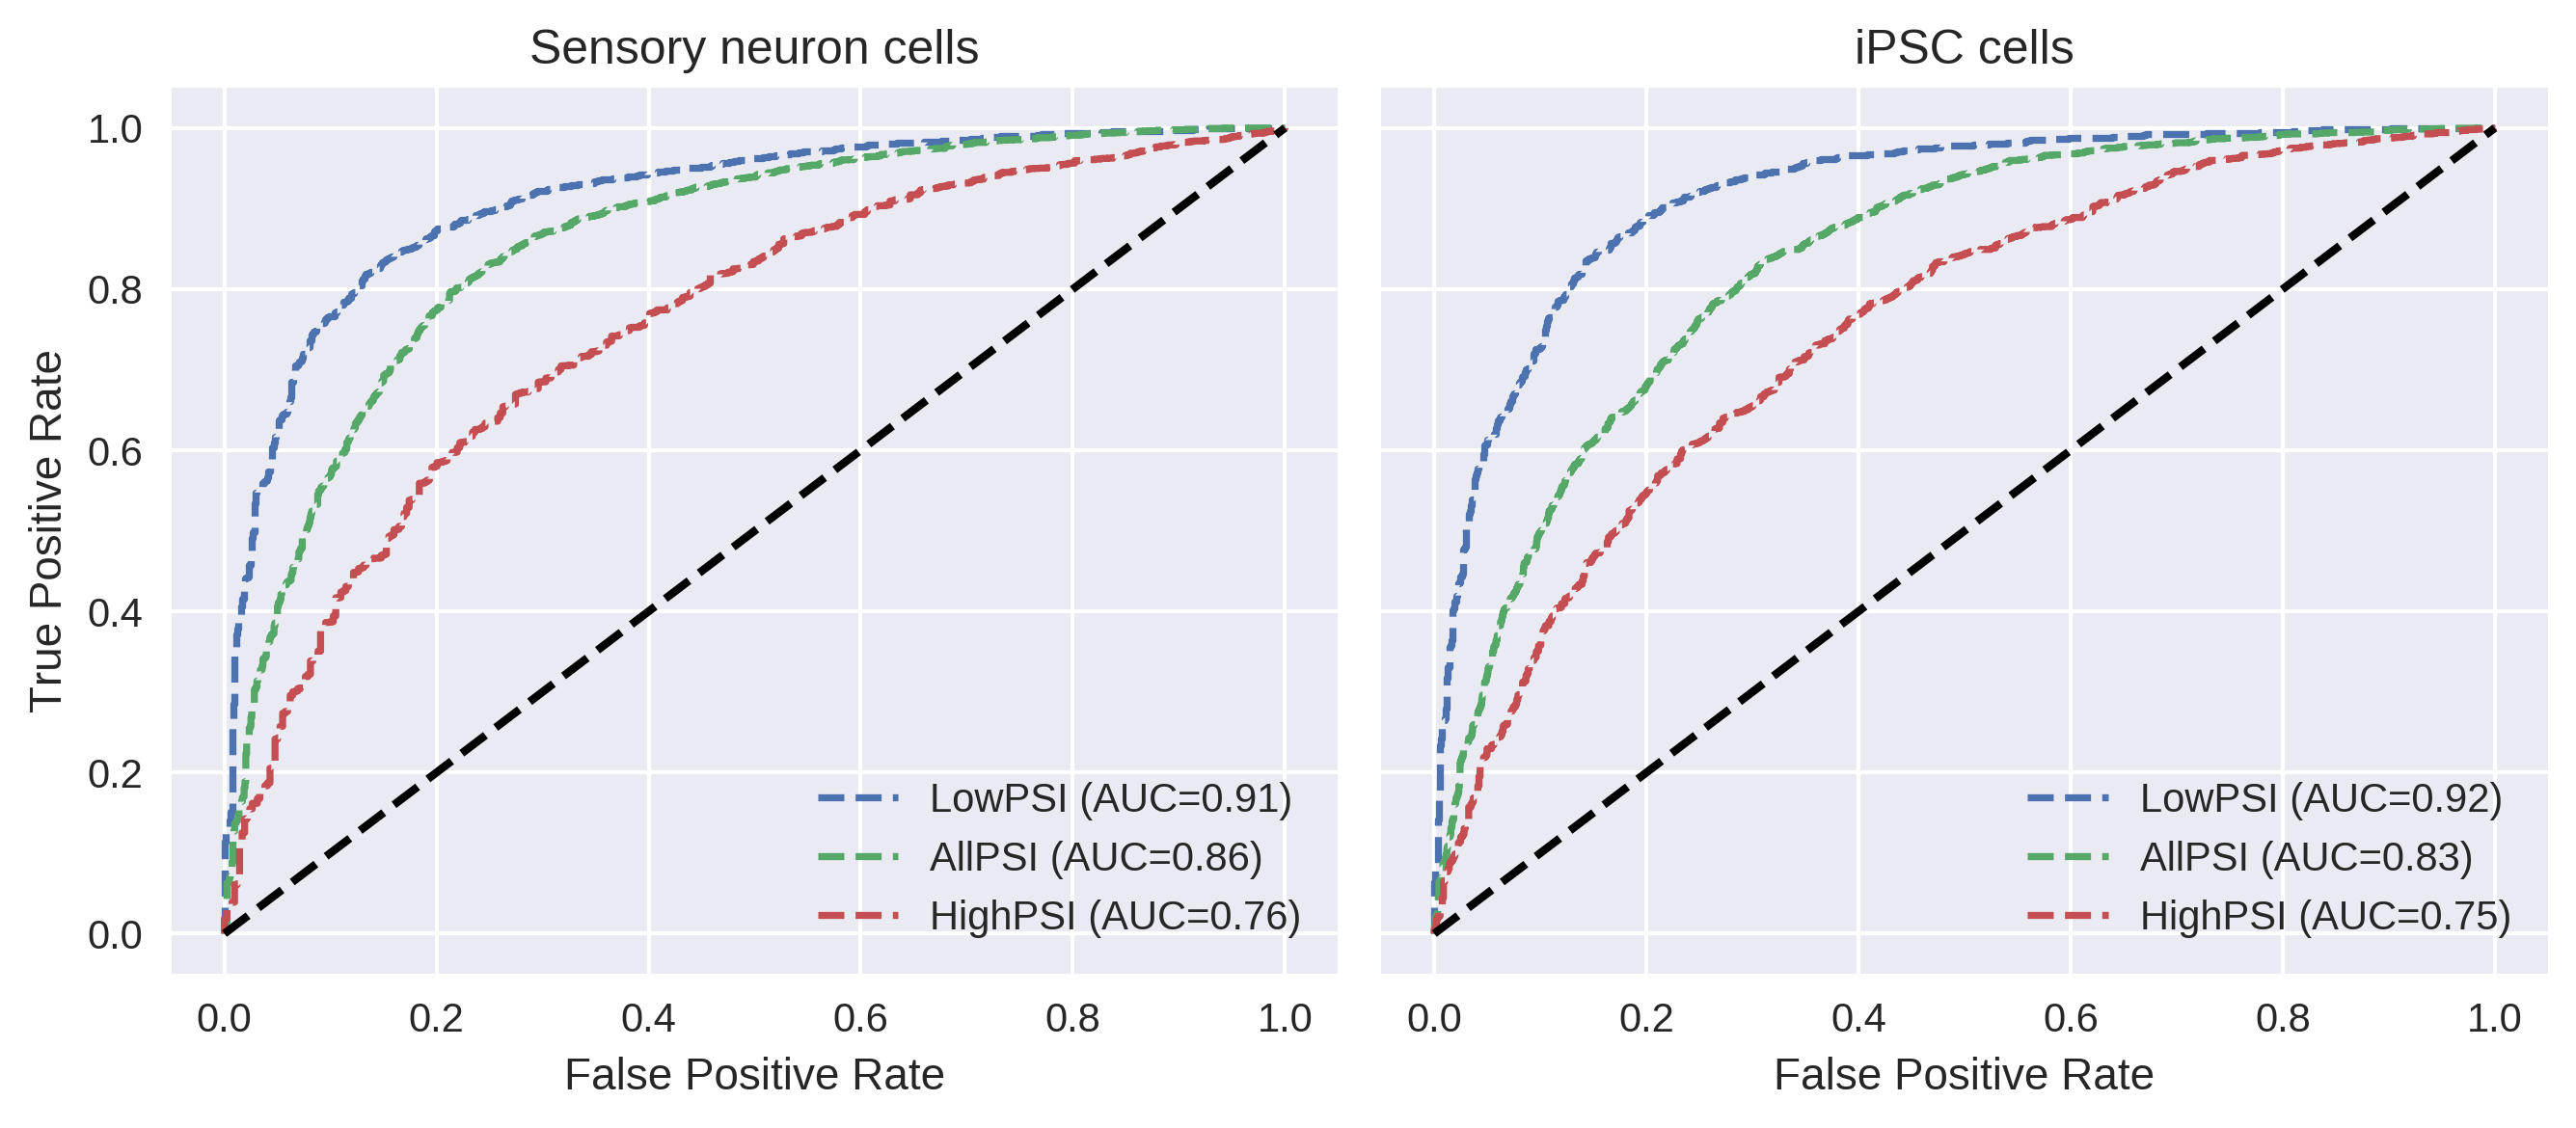
\includegraphics[width=1\textwidth]{../visualizations/ch5-results/majiq_neuron_ipsc_cross_psi_roc_auc_comparison.png} 
	\caption{Left: ROC curves on HipSCi MAJIQ dataset derived from iPSCs differentiated to neurons. Right: ROC curves on HipSCi MAJIQ dataset derived from undifferentiated iPSCs. }
	\label{fig:majiq_rocs_low_high}
\end{figure}
%The dataset based on undifferentiated iPSCs seems to be less challenging: the AUCs are roughly 0.02 higher than on the dataset based on sensory neuron cells. At a closer look at the dataset distribution....

% dataset composition:
% neuron: 26394 / 8201 / 10151 = 44746
% ipsc: 27371 / 9299 / 11819 = 48489
% --> look at relative numbers, once you have analyzed across tissue-performance

% change roc curves such that I give AUC values explicitly (better than alternative of redoing)


\subsubsection{Impact of architectural choices} \label{subsubsec:majiq_architectural_choices}
The poor performance of D2V is likely a result of its architecture: the 100-dimensional embeddings used for classification weren't optimized jointly during training and likely don't contain fine-grained information, such as the specific positons of motifs, required for accurate splicing prediction. We conjecture that D2V would benefit from receiving further split input sequences, e.g. input sequences containing 35 nucleotides. The best solution, while keeping the word embeddings, would likely be to embed the overlapping 3-mers in the sequence via word2vec and combine this with an efficient convolutional architecture, as done in \cite{d2vsplicing}.



\subsubsection{Assessing the dataset quality}

\begin{table}[h!]
	\centering
	\resizebox{\textwidth}{!}{\begin{tabular}{| l | c | c | c| c} 
		\hline
		Model name & Only sequences & Sequences + lengths & Relative gain\\
		\hline
		DSC & 0.811 & 0.808 & -1.0\%\\
		D2V & 0.665 & 0.715 & 23.3\%\\
		RASC & \textbf{0.853} & \textbf{0.865} & 3.3\%\\
		\hline
	\end{tabular}}
	\caption{
		Performance on the sensory neuron cell-based HipSci MAJIQ dataset with and without length features given. 
%		Performance on the dataset based on processing with MAJIQ and iPSCs differentiated to neurons with and without length features given. 
		%		Note that the relative performance drop was computed with reference to the baseline AUC value of 0.5.
	}
	\label{table:majiq_nolens}
\end{table}

As litmus test for dataset quality, we repeat the experiment of removing the length features as model input. We document the results in Table \ref{table:majiq_nolens}.
They reveal that a large part of D2V's performance relies on information contained in the length features. However, since removing the length features only marginally affects the performance of DSC and RASC, we conclude that this observation is symptomatic of D2V being unable to effectively incorporate information from the sequences (see discussion in \ref{subsubsec:majiq_architectural_choices}), rather than the dataset being biased in the same way as the HEXEvent dataset.  

Given a) the strong model performance independent of the length features and b) the prior expectation for MAJIQ to produce the highest quality PSI estimates, we conclude that it does. This indicates that the comparatively poor performance on the GTEx-based and HipSci SUPPA datasets are due to poor data quality, and not due to the inherent difficulty of the splicing classification task. Thus, using the HipSci MAJIQ datasets is preferable to using any of the other datasets we have evaluated. 

Motivated by this observation, we use the HipSci MAJIQ dataset to validate our architectural choices for RASC and to carry out further analysis omitted on the other datasets.





\subsection{Evaluation of the additional attention modifications} \label{subsubsec:attn_hyperparams}

We evaluate the three additional attention modifications described in \ref{subsec:alternative_attention} by testing them sequentially. The results of these tests are shown in Figure \ref{fig:attn_extension_barcharts}. 

\begin{figure}
	\centering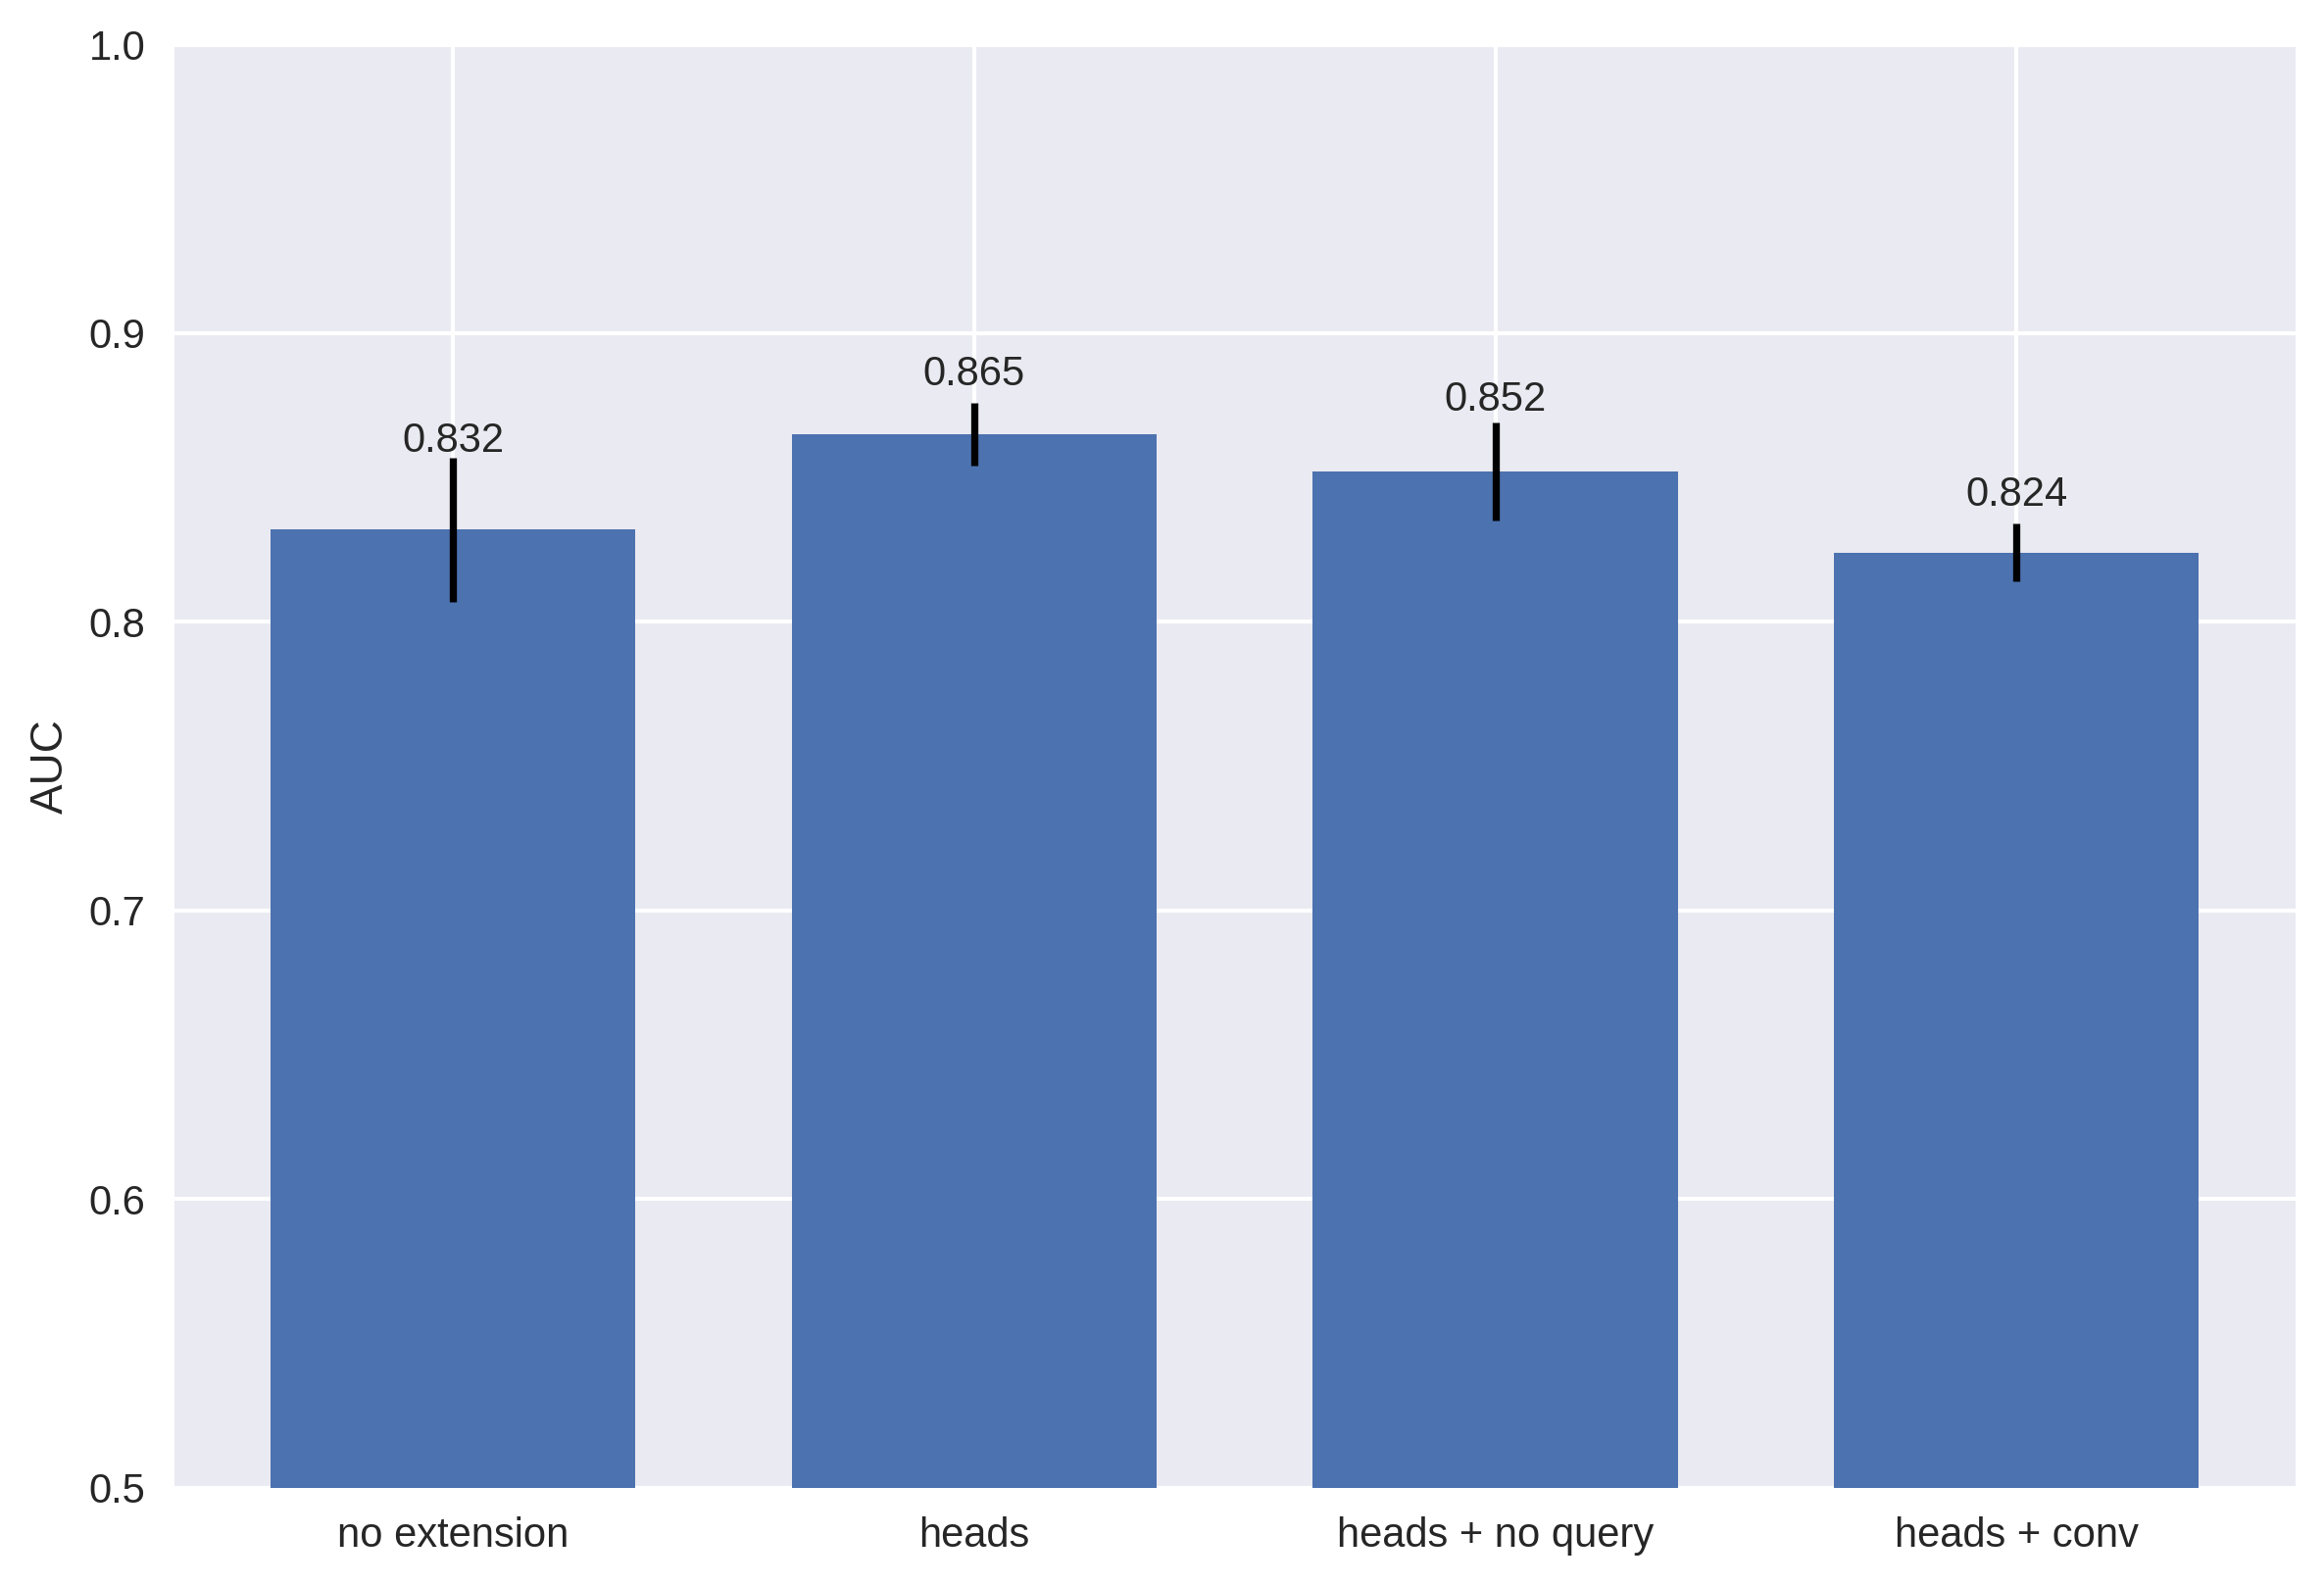
\includegraphics[width=1\textwidth]{../visualizations/ch5-results/attn_extension_barcharts.png} 
	\caption{Performance evaluation of the three extensions to the attention mechanism. We abbreviate the use of multiple attention heads as `heads', the removal of the query matrix as `no query' and the introduction of an additional convolution as `conv'. }
	\label{fig:attn_extension_barcharts}
\end{figure}


%compute average of conv training error: 0.9884710561726501 for conv + no query

%
%\begin{table}[h!]
%	\centering
%	\begin{tabular}{| c c c | c c | c} 
%		\hline
%		%   & configuration & & performance & \\
%		heads & no query & conv & $\mu$ & $\sigma$ \\
%		\hline
%		0 & 0 & 0 & 0.832 & 0.025 \\
%		0 & 0 & 1 & 0.860 & 0.021 \\
%		0 & 1 & 0 & 0.851 & 0.013 \\
%		0 & 1 & 1 & 0.818 & 0.019 \\
%		1 & 0 & 0 & \textbf{0.865} & 0.011 \\
%		1 & 0 & 1 & 0.824 & \textbf{0.010} \\
%		1 & 1 & 0 & 0.852 & 0.017 \\
%		1 & 1 & 1 & 0.846 & 0.017 \\
%		\hline
%	\end{tabular}
%	\caption{Results of evaluating the three additional attention extensions. $\mu$ denotes the average AUC across 9 experiments and $\sigma$ the respective standard deviation. 0 codes for the extension not being used, 1 codes for the extension being used. The extensions were abbreviated as follows: heads = multiple attention heads were used, no query = no conceptual query matrix was used, conv = an additional convolution operation was applied to the key and value matrices.
%	}
%	\label{table:attn_extensions}
%\end{table}
\subsubsection{Using multiple attention heads} \label{subsubsec:result_heads}
Using multiple attention heads leads to significantly improved performance and to significantly reduced variance between runs. Thus, the additional representational subspaces appear to improve performance and the ensemble model effect of multiple attention heads appear to reduce variance. No overfitting is observed, despite the number of model weights increasing from roughly 36,000 to 67,000 compared to the single attention head model. Due to the uniformly improved performance, we elect to incorporate multiple attention heads into RASC. 

%36361 -> 66861 

\subsubsection{Removing the query matrix}  % 56465 parameters
We observe slightly diminished performance upon removing the query matrix. The extra representational capacity afforded to RASC by having query matrices appears to improve its predictive power. Despite decreasing model size by roughly 10,000 parameters when removing the query matrices, we decide to not incorporate this adaption of the attention mechanism. 

%However, in initial experiments, the attention** mechanism performed significantly worse than the attention* mechanism. The extra representational capacity by having a query matrix seems to be important for performance. 
%In practice, this lead to a model about 10\% smaller. 
%In practice, this lead to an about 10\% smaller model.

%all 8 possible variations of combining them. Quantitative results are reported in Table \ref{table:attn_extensions}. 
%The overall best performing model uses multiple attention heads, but no other extensions. Using multiple attention heads appears to make the model perform consistently better than the baseline, except when paired with the convolution extension. On a closer look, this seems to be the result of the model overfitting to the dataset as shown in Figure [...]. %TODO
\subsubsection{Adding an extra convolution}
Adding an additional convolution operation to the attention mechanism, surprisingly leads to decreased performance, even comparing unfavorably to the baseline single-head attention model. This in contrast to \cite{ghentransformers} where this extension lead to very significant relative performance improvements. There are likely multiple factors contributing to these varying results:
% Reasons for why this extension did not work might be related to the use of a recurrent encoder as well as task differences:

\begin{figure}
	\centering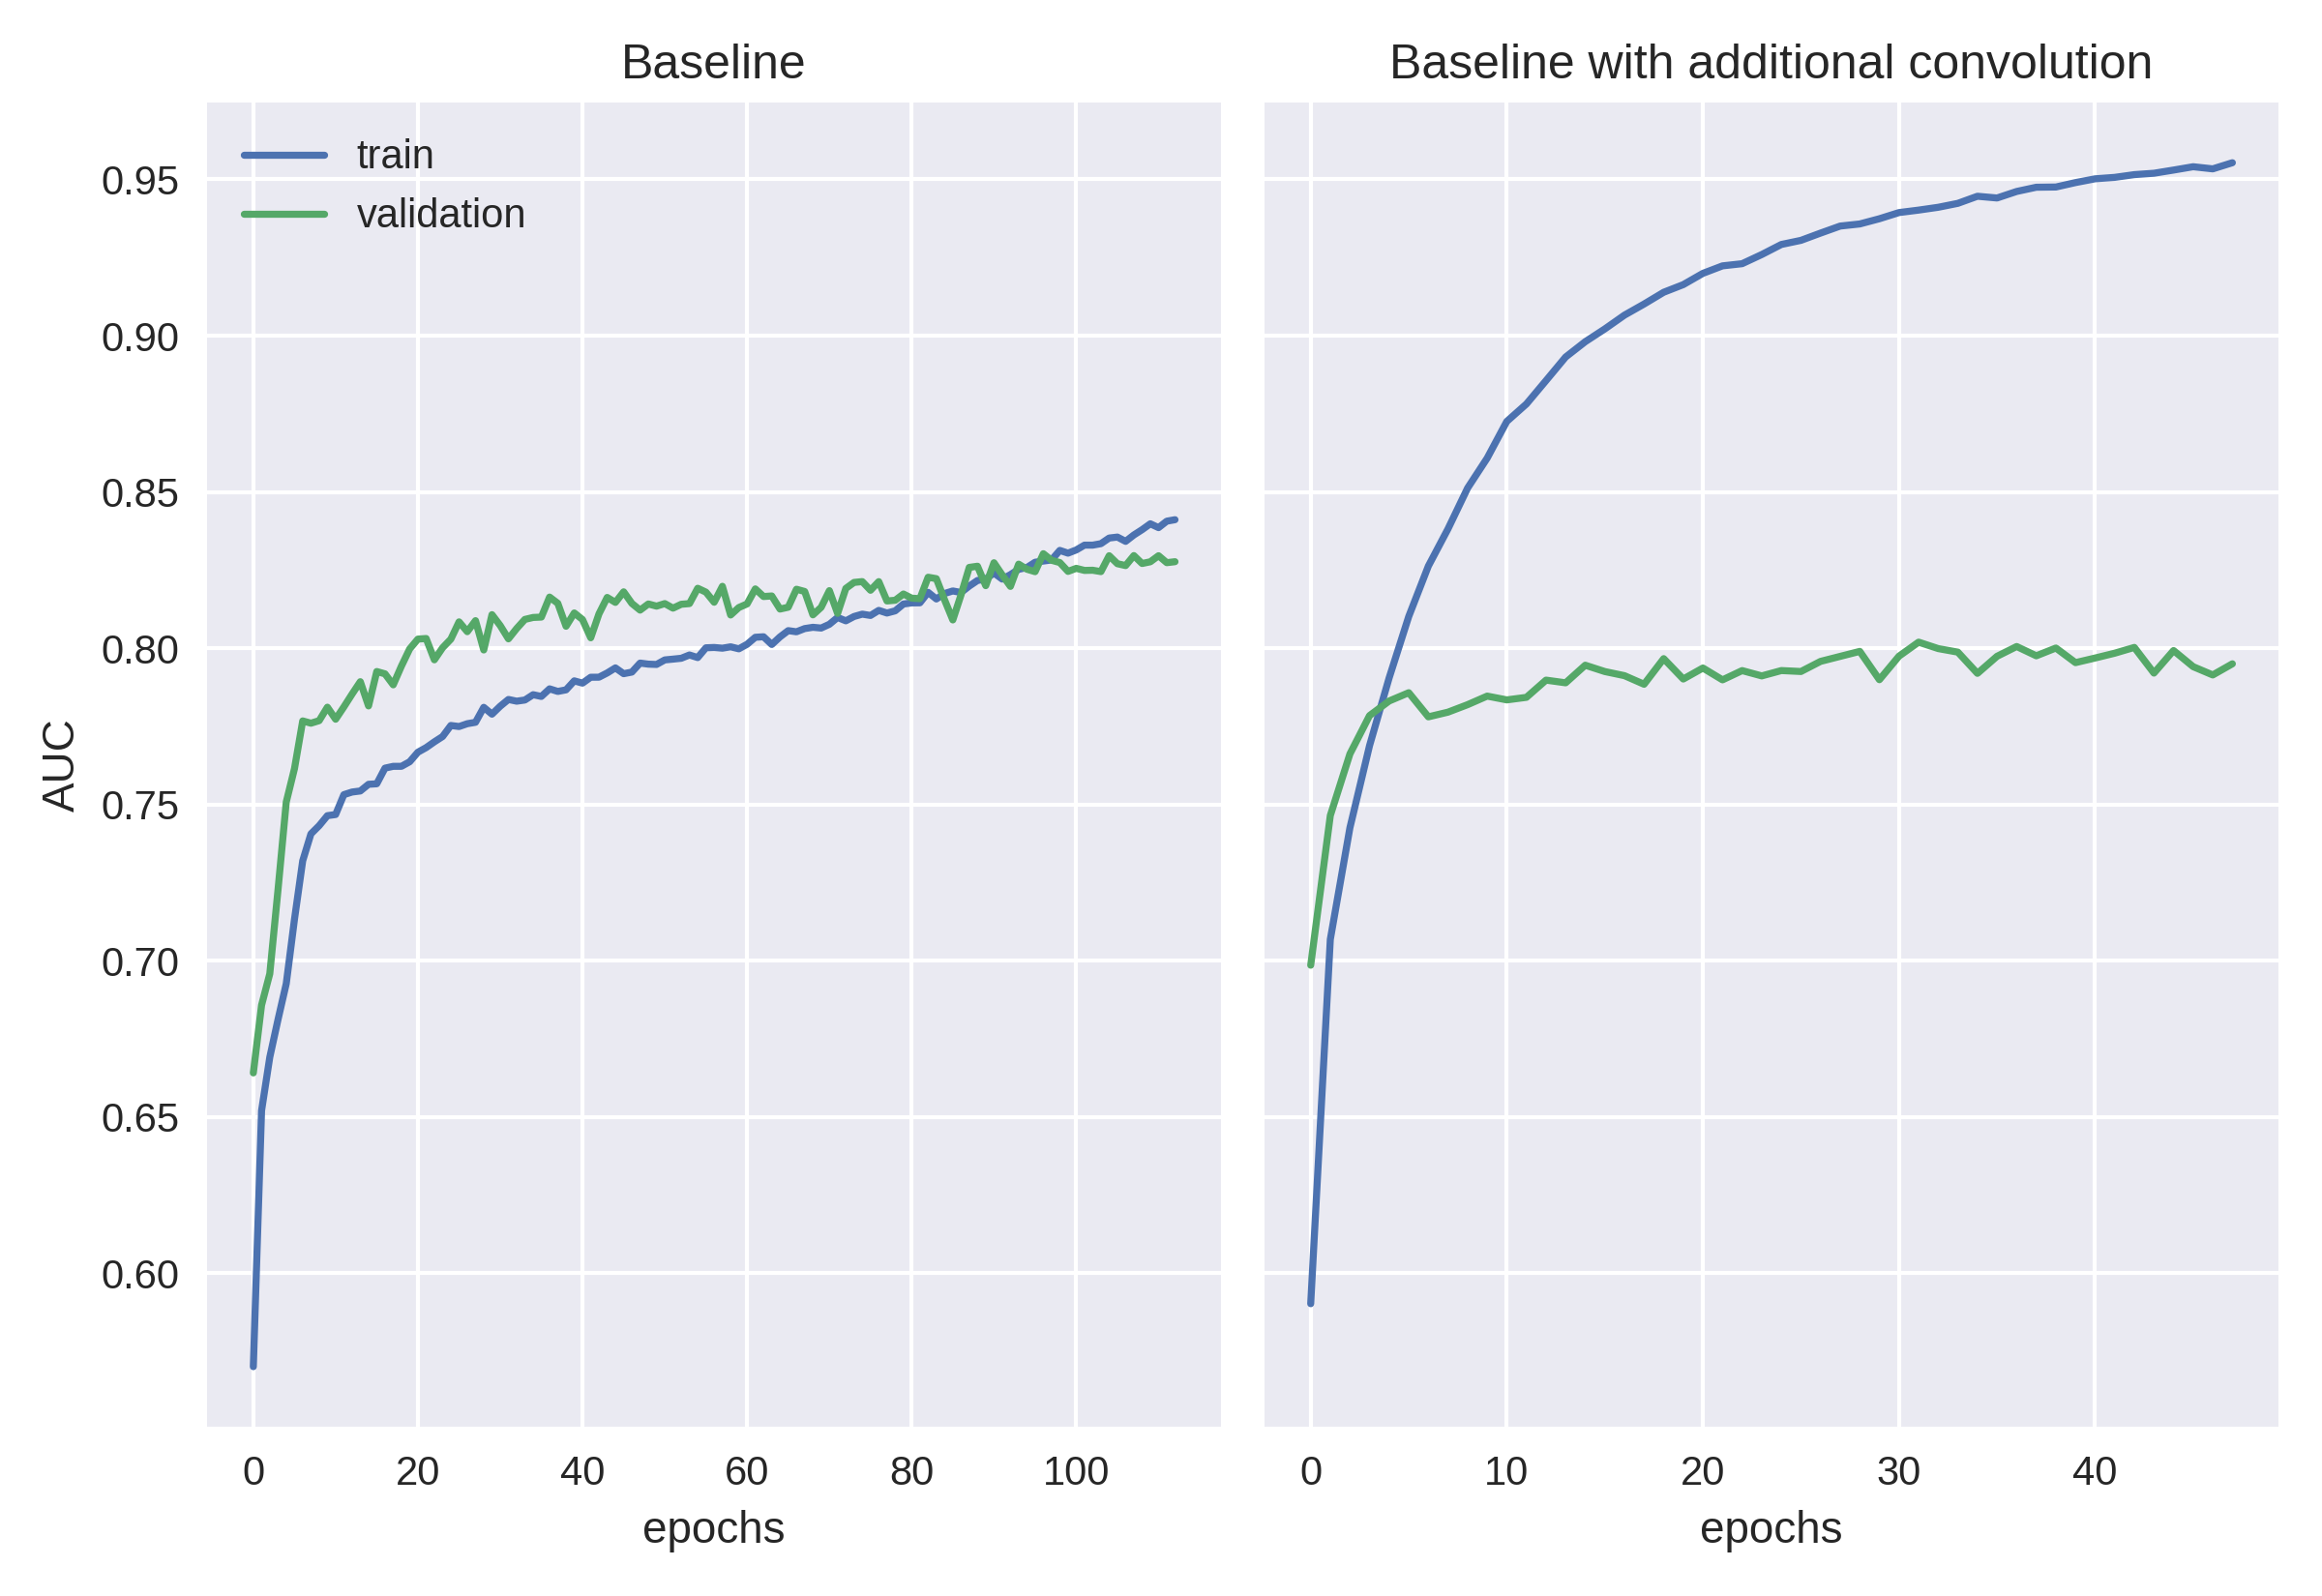
\includegraphics[width=1\textwidth]{../visualizations/ch5-results/training_curve_conv_heads2.png} 
	\caption{RASC overfits when the additional convolution operation is introduced into the attention heads. The baseline refers to RASC with multiple attention heads. }
	\label{fig:training_curve}
\end{figure}


\begin{enumerate}
	\item Although we process the input at single-nucleotide resolution, the use of a BiLSTM unit means that the encoder is aware of the nucleotides which precede and follow it. Therefore, the model can already encode information about the neighbouring nucleotides in the representation for a given nucleotide. This is in contrast to a Transformer model where the layers are non-recurrent and only work at single-nucleotide resolution. Thus, the convolutional layers likely give the model less additional modelling flexibility.
	\item In \cite{ghentransformers}, a 3000 nucleotide context window is processed through 6 attention layers (so 500 nucleotides per layer). In our work, a 280 nucleotide context window is processed through 1 attention layer. Thus, one attention layer in RASC needs to integrate information from fewer nucleotides. Thus, RASC might need less additional capacity to integrate evidence from multiple nucleotides than \cite{ghentransformers}'s model. 
%	  are given to the model. In contrast, we only give 280 nucleotides to our model. Thus, the additional capacity 
	
%	\item In \cite{ghentransformers}, the task is full genome transcription start site annotation (so predicting where genes start). Therefore, their task occurs at the inter-gene level while our task occurs at the intra-gene level. This likely means that the motives \cite{ghentransformers}'s model has to consider generally span more nucleotides and granting the model more capacity to integrate information over multiple nucleotides is more crucial. 
%	In contrast, granting RASC more capacity to integrate information over multiple nucleotides may not be necessary to identify the shorter motifs influencing splicing. 

%	In contrast, the comparably fine-grained working of RASC may be necessary for it to identify the shorter motifs which influence splicing. 
%	Thus, these differences likely also influenced the performance differences when using the convolutional attention layer extension in the different models.
	%		they: 3000 nucleotides, convolution filter of 7
	\item Furthermore, we observe overfitting when using this extension. The training curve in Figure \ref{fig:training_curve}
	showcases this behaviour. We observe overfitting despite using the same convolution across multiple heads, increasing the dropout probability in the attention heads, introducing additional batch normalization layers and limiting the convolution kernel size to 3.
	%(see Table \ref{app:conv_tests} in the appendix for further results)
\end{enumerate}


In summary, we extend RASC with multiple attention heads. The results of RASC we report on the other datasets also use the model with multiple attention heads. 


%\subsection{MAJIQ with iPSCs differentiated to neurons (junctions)}
%haven't run experiments yet, not sure if results are interesting (but probably yes)\\
%due to training times, probably don't want to run these with cross-validation as that would take 15 hours+

\subsection{Sensitivity and specificity analysis}
\begin{figure}
	\centering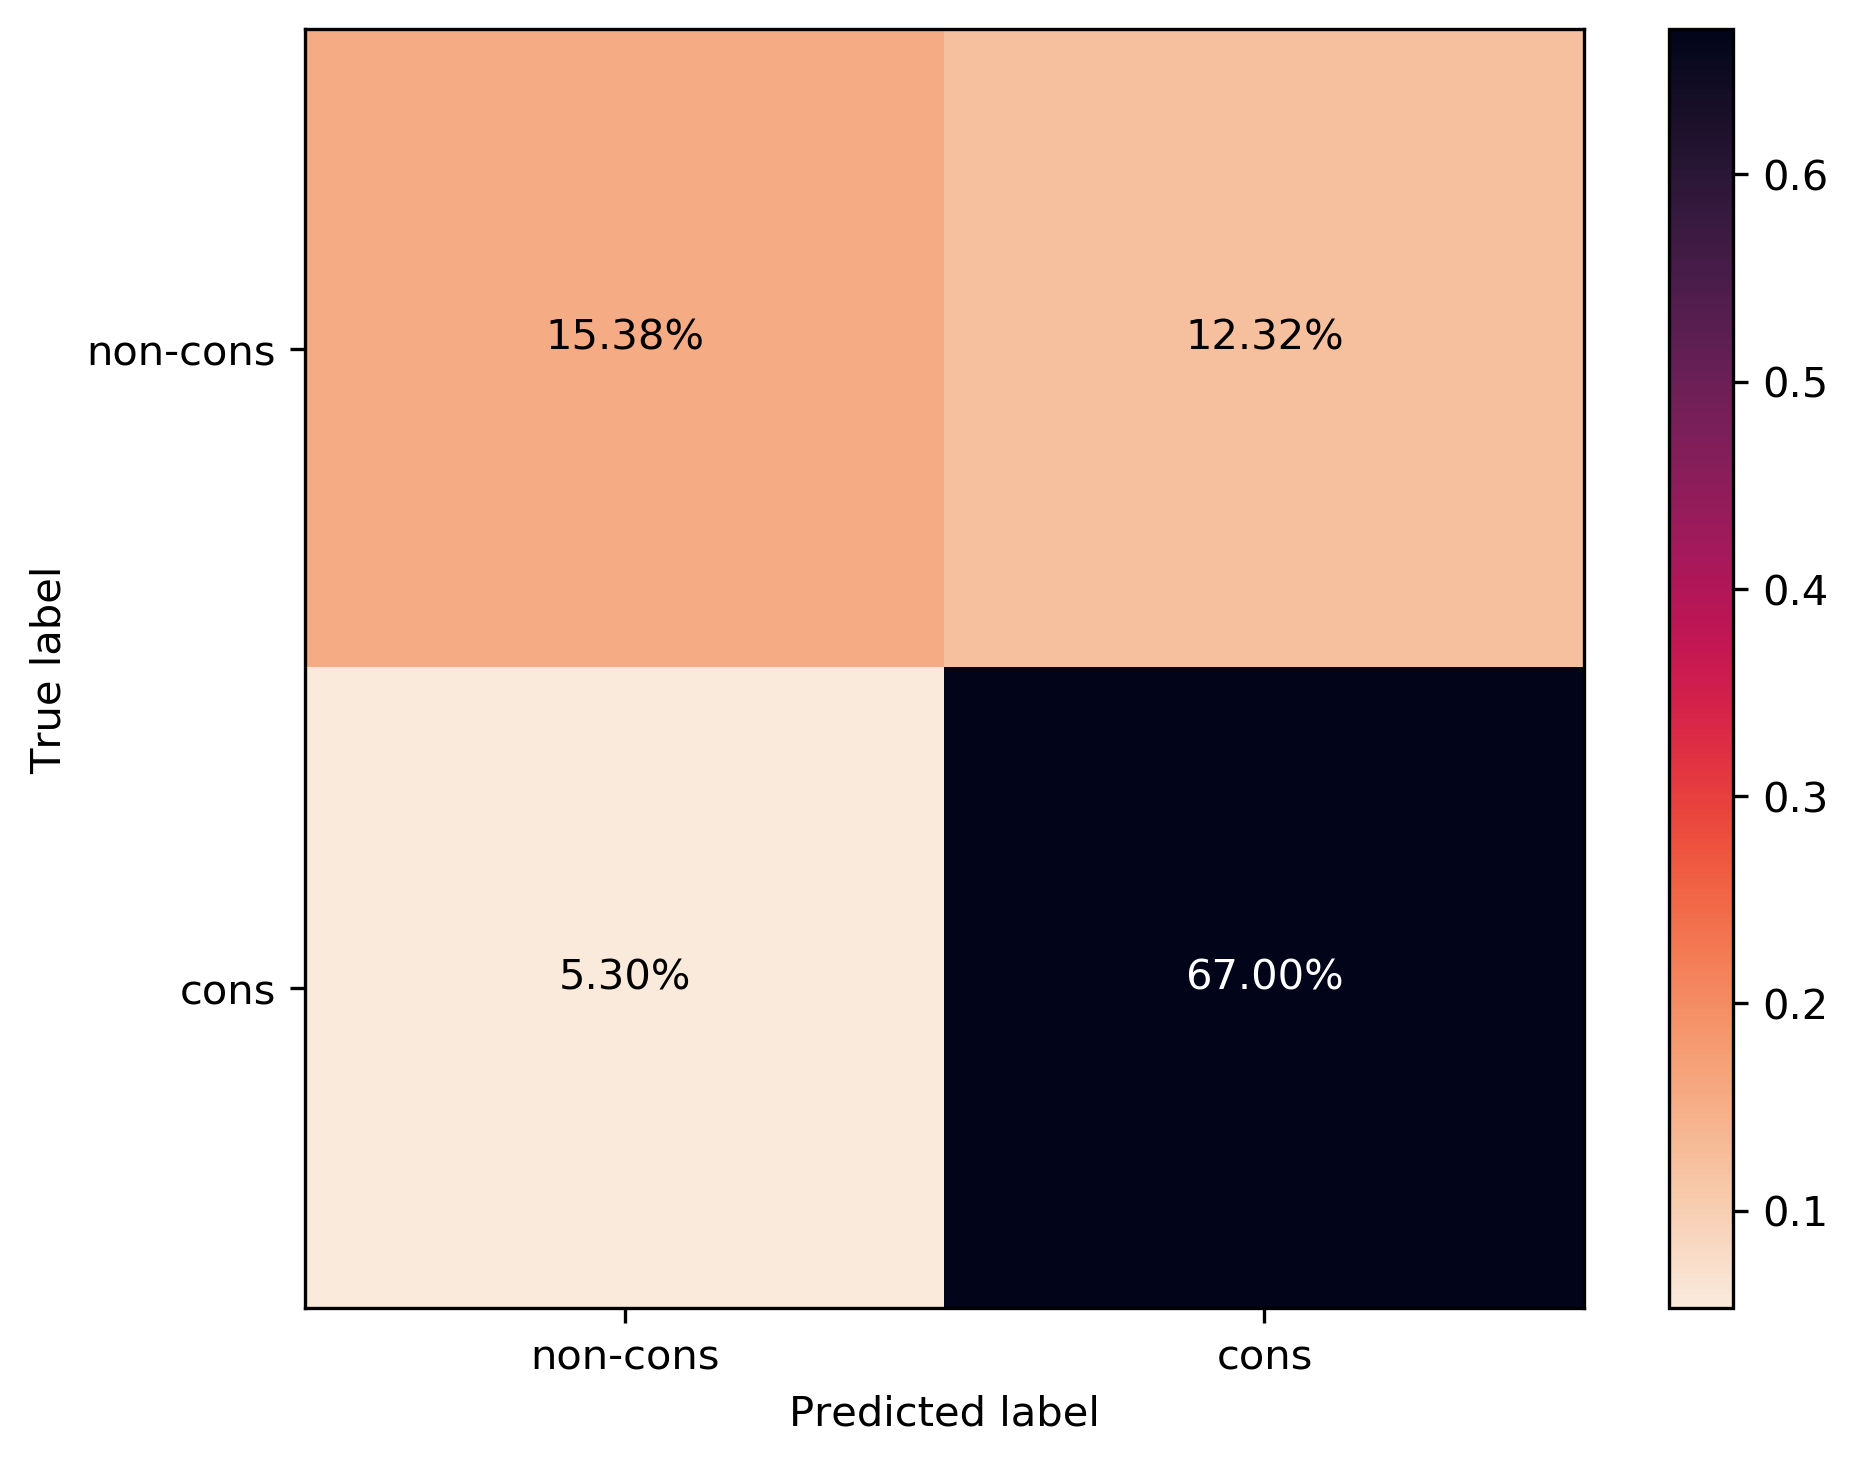
\includegraphics[width=0.7\textwidth]{../visualizations/ch5-results/confusion_matrix.png} 
	\caption{Confusion matrix from RASC on the neuron HipSci MAJIQ dataset. `cons' and `non-cons' respectively abbreviate constitutive and non-constitutive exons. }
	\label{fig:confusion_matrix}
\end{figure}

We present the confusion matrix for the binary classifier based on RASC in Figure \ref{fig:confusion_matrix}. The decision threshold which maximizes the F1 score was chosen resulting in a F1 score of 0.88 (for the negative class of constitutive exons) and classification accuracy of 82\%. We observe comparatively few false positives, but many false negatives and correspondingly obtain a low sensitivity score of 0.56, but a high specificity score of 0.93. Thus, the classifier performs well at ruling in that an exon is alternatively spliced, but poorly at ruling that it isn't. This means the classifier is attractive for guiding the investigation of exons, where it wasn't previously known that they are alternatively spliced. This wouldn't be possible with a less specific classifier because further investigation relies on expensive wet-labs experiments for which the number of false positives need to be minimized. When employing RASC in practice, the decision threshold should be chosen such that the specificity is even higher (at the cost of further reduced sensitivity): a false positive rate of 5.3\% is still too high for wet lab experiments. Thus, we conclude that our classifier shows attractive properties, but would require further tuning before practical use. 
% todo (maybe): actually evaluate other decision thresholds here

%              precision    recall  f1-score   support
%cons       0.74      0.56      0.64      1239
%non-cons       0.84      0.93      0.88      3234
%accuracy                           0.82      4473


% sensitivity: 0.56 -- ruling out alternatively spliced
% specificity: 0.93 -- ruling in alternative spliced
% f1 score: 0.88, precision: 0.845 (cons), recall (cons): 0.927


\subsection{Cross-condition performance} \label{subsec:hipsci_ipsc_majiq}

\begin{figure}
	\centering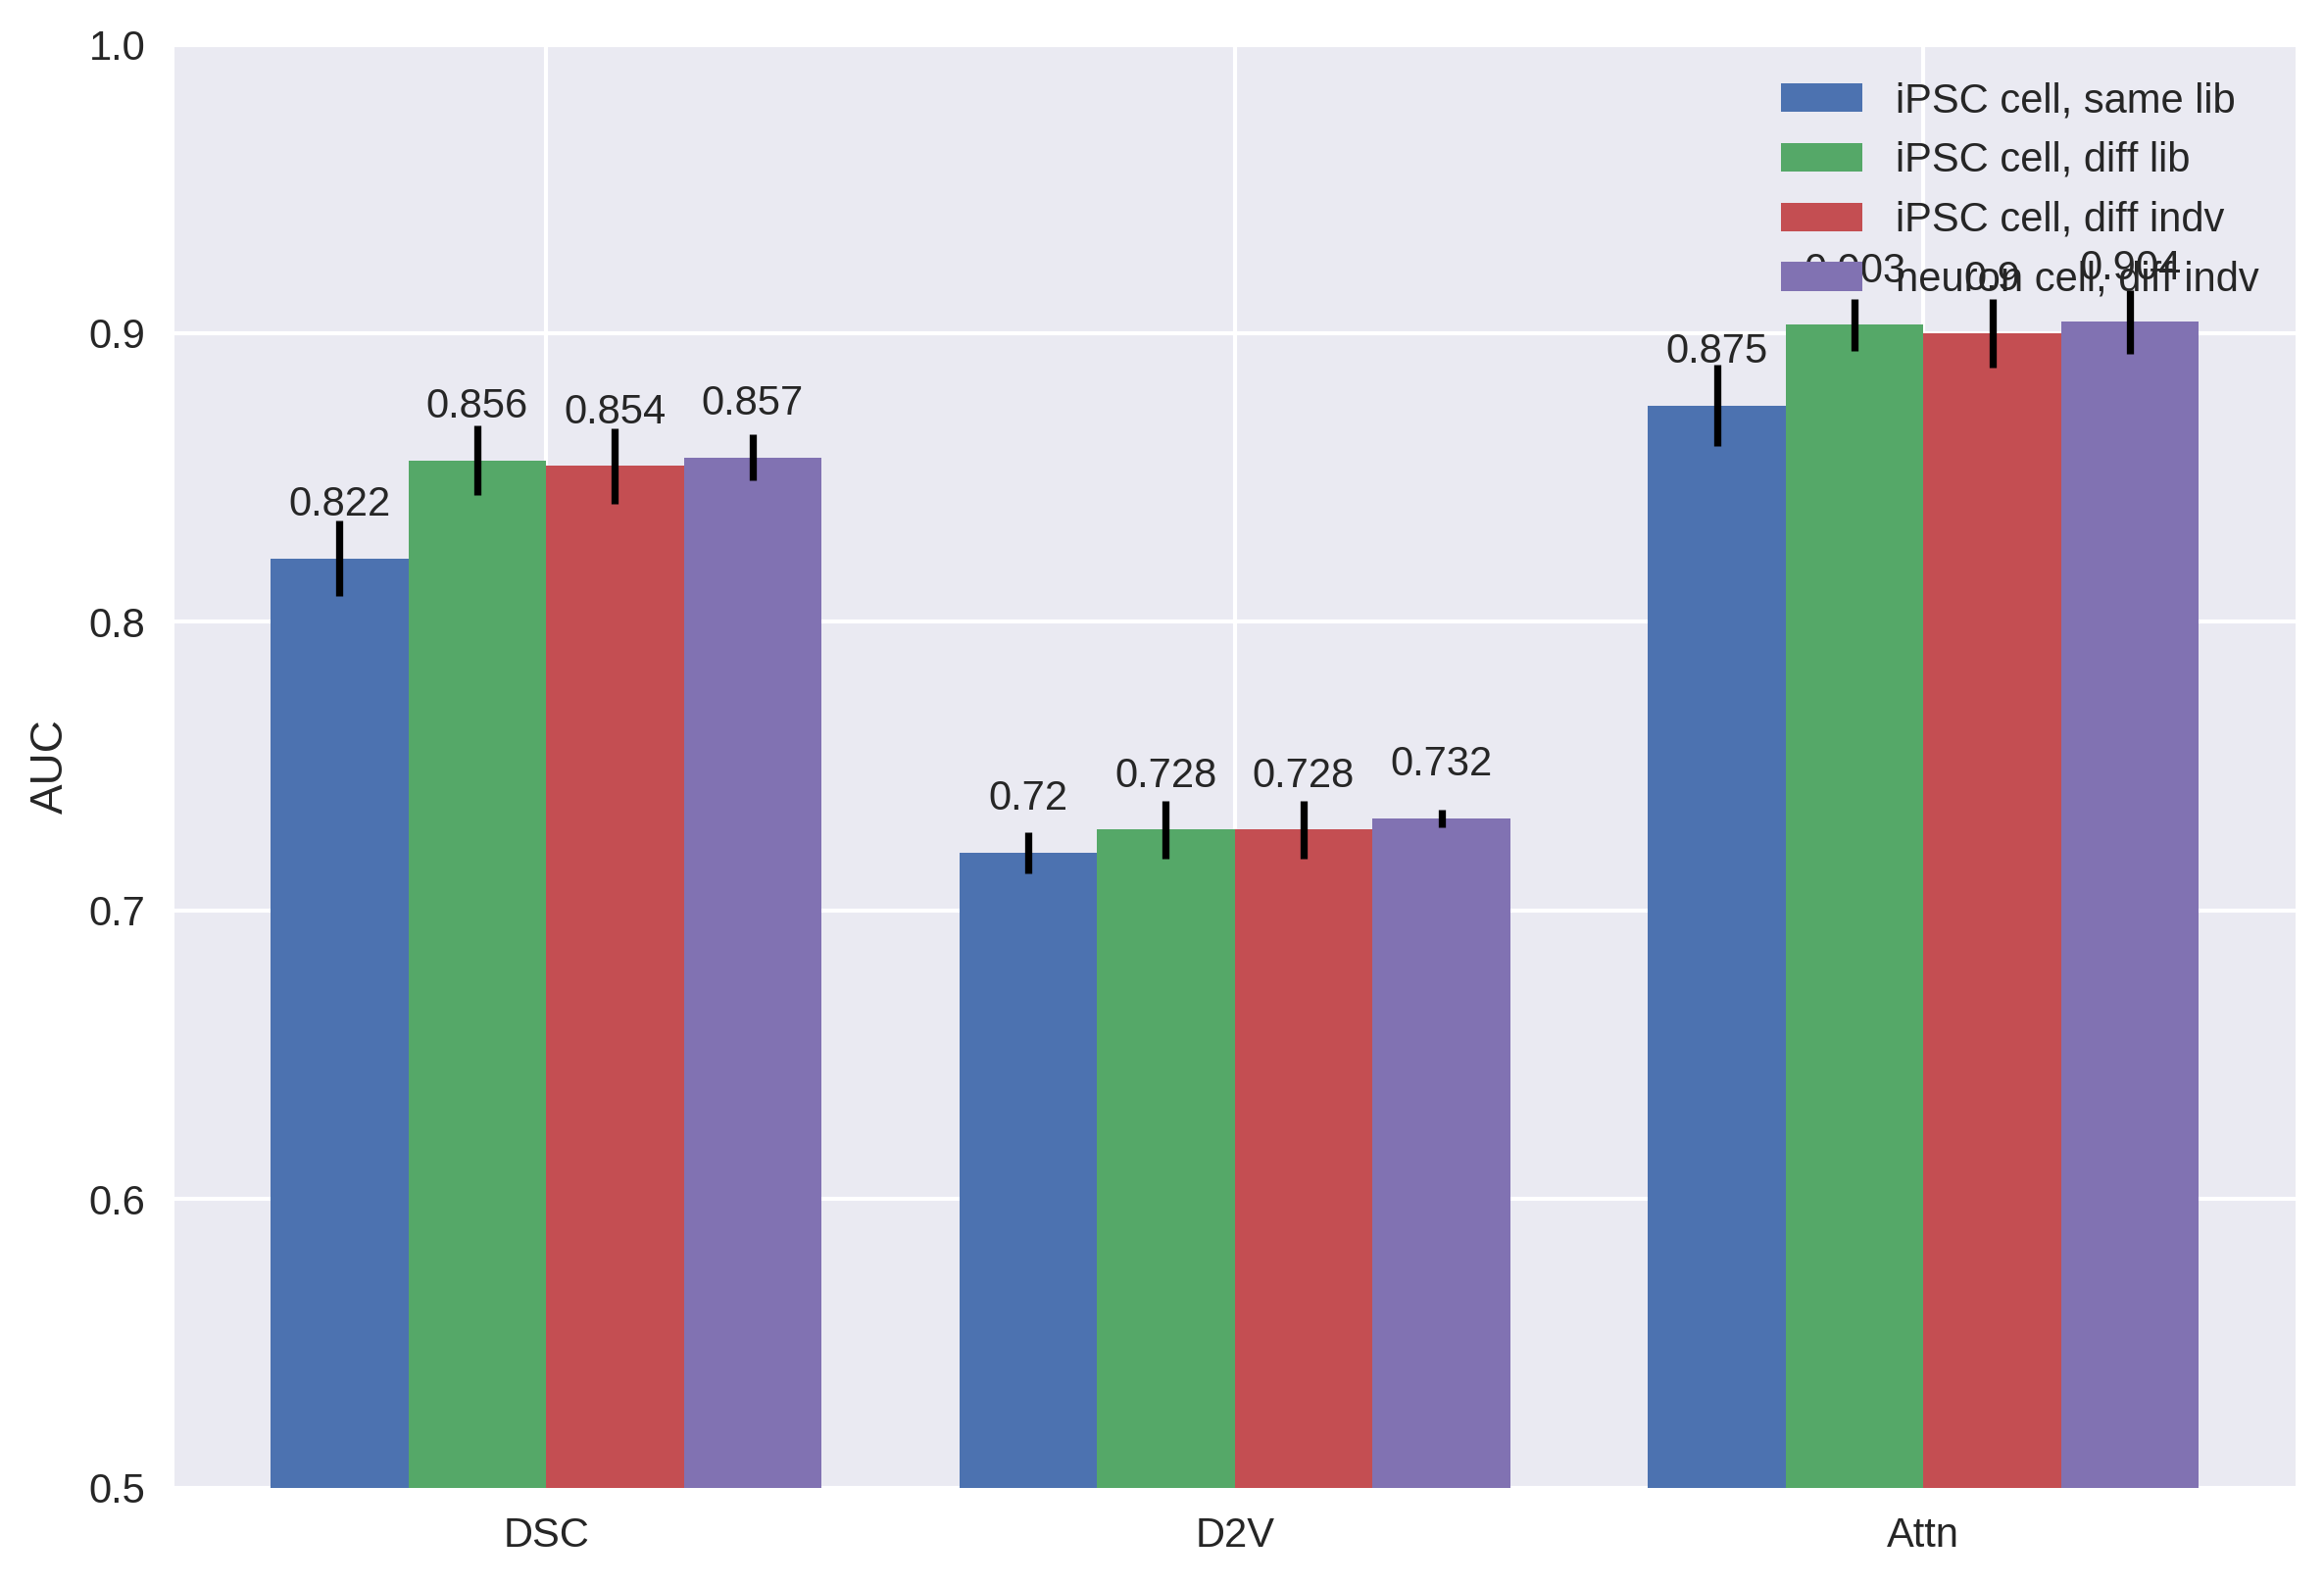
\includegraphics[width=0.85\textwidth]{../visualizations/ch5-results/majiq_comparison_barcharts.png} 
	\caption{Performance when training models on one HipSci dataset and testing on the same dataset as well as three others. Within the bars of one model, going further right means using a dataset which is less similar to the dataset the model was trained on (the left-most bar display performance when testing the model on the dataset it was trained on). `lib' refers to a library or biological sample from the same individual, `indv' refers to the indivdiual the sample was taken from, `diff' abbreviates different. `iPSC' refers to a dataset based on RNA-seq data from undifferentiated iPSCs while `neuron cell' refers to iPSCs differentiated to sensory neuron cells. }
	\label{fig:majiq_comparison_barcharts}
\end{figure}


We evaluate how well the models generalize when trained on a dataset derived from one individual and then tested on a dataset derived\footnote{When choosing the samples to evaluate on from the different datasets, care needs to be taken to avoid a subtle data leak: despite the different primary data sources, many of the cassette exons appear as training samples in multipe datasets. %are duplicated of the same exons occur in final training samples.
%	 are 
%	many training samples are shared betwee
%	due to the specifics of MAJIQ, the original dataset and the dataset from the same individual but a different library share the consecutive exon training samples. 
	This initially lead to the surprising observation that it is better to train on a dataset different from the one the model is evaluated on. We avoid this issue by efficiently filtering all samples that are in the original training dataset from the three additional datasets via a hash set.}
\begin{itemize}
	\item from the same individual, but a different library.
	\item from a different individual, but the same cell type.
	\item from a different individual from a different cell type.
\end{itemize}


We visualize the results in Figure \ref{fig:majiq_comparison_barcharts}.
Unsurprisingly, performance generally drops when a model is evaluated on a dataset different from the one it was trained on. Surprisingly, this performance drop does not directly correlate with the similarity to the original dataset: the least similar dataset from a different tissue performs best. 
This is because the baseline performance on the sensory neuron dataset is roughly 2\% higher and it experiences only a roughly 1\% higher performance drop when training was done on a different dataset. The models generalize extremely well across tissues and conditions. As previously suggested, this is biologically surprising due to known splicing differences between tissues \cite{crosstissuesplicing}. Possibly the datasets don't capture the splicing behaviour which is different across tissues.


%This means that the splicing behaviour learned on one tissue generalizes extremely shows that the splicing behaviour 

%iPSC_D2V_MLP	0.711	0.007	0.756	0.010	0.675	0.006
%iPSC_Attn	0.846	0.007	0.933	0.006	0.765	0.009
%iPSC_DSC	0.785	0.010	0.856	0.010	0.720	0.012
%MultiHeads	0.865	0.011	0.919	0.018	0.768	0.018
%HIPSCI_MAJIQ_DSC	0.808	0.010	0.850	0.011	0.721	0.010
%HIPSCI_MAJIQ_D2V_MLP	0.715	0.007	0.741	0.007	0.672	0.014

% 865 - 846 = 019
% 2, 2, 
%Coupled with \ref{fig:majiq_rocs} showing that performance when training and evaluating on the sensory neuron cells dataset is higher than that of the iPSC dataset too, we conclude that the splicing behaviour derived from sensory neuron cell data is easier to predict. 
%idea: substract performance from sensory too -- what do we get? 


%The performance drop when evaluating on a dataset from a different library or a different individual is the same and bewteen 2\% to 4\% for all models. In this instance, such a moderate performance drop is not surprising due to the similaritie


However, to more seriously investigate how splicing differs between conditions and tissues, the capability of MAJIQ to quantify differential splicing should be taken advantage of. The best performing model, RASC, could be adapted such that it takes in an exon as well as two different conditions (e.g. via one-hot encoded tissues) and then predicts the change in splicing behaviour between the two conditions. 


%- constitutive exons are shared across all datasets
%- majiq builder builds up initial splice graph using all samples -- some confounding there for sure
%- for this sort of analysis, prediting differential splicing itself would be more apt
%
%cross-tissue comparison here with very low variance across tissues;\\
%seems like learned features are mostly tissue-invariant\\

















\subsection{PSI Regression} \label{subsubsec:psi_regression}
After having achieved a good level of performance on the classification task, we turn to the regression task. We train the models on the sensory neuron cell HipSci MAJIQ dataset and give the results in Table \ref{table:psi_regression}. 


\begin{table}
	\centering
	\begin{tabular}{ c c c c c c c} 
		\hline
		Model & AllPSI &  LowPSI &  HighPSI \\
		\hline
		DSC	&	0.244   $\pm$	0.036	&	0.340	$\pm$	0.039	&	-77.980	$\pm$	13.631\\
		D2V	&	0.120	$\pm$	0.009	&	0.155	$\pm$	0.010	&	-57.523	$\pm$	2.771\\
		RASC	&	\textbf{0.486}	$\pm$	0.067	&	\textbf{0.595}	$\pm$	0.074	&	\textbf{-25.470}	$\pm$	5.717\\
		\hline
	\end{tabular}
	\caption{Mean $R^2$ for PSI regression task on sensory neuron cell HipSci MAJIQ dataset.  $\pm$ denotes standard deviation. 
	}
	\label{table:psi_regression}
\end{table}


The results show that the models still fail to explain a lot of the variation in the PSI value: no model is able to explain even half of it. 
As on the classification tasks, RASC outperforms the other models by a wide margin and all models are significantly worse on explaining the variance for highly included, rather than rarely to moderately included, non-constitutive exons. The latter observation is particularly pronounced: the $R^2$ score of all models on HighPSI is below 0, showing that they fail to explain the variance even as well as a baseline model whom consistently predicts the mean. Thus, we take these results as indication that the current Splicing Codes can still be significantly improved. 



%We generally observe poor to middling performance: DSC and D2V don't beat the baseline model with . Again, RASC outperforms the other models by a wide margin. 
%Like in the exon classification task, all models perform significantly worse on highly than on rarely to moderately included non-constitutive exons. 

\begin{table}
	\centering
	\begin{tabular}{ l c c c c c c} 
		\hline
		Model & Performance \\
		\hline
		BNN-UDC \cite{jha} & 0.220\\
		BNN-LMH \cite{jha}& 0.368\\
		DNN-PSI \cite{jha} & 0.434\\
		D2V \cite{d2vsplicing} & 0.594\\
		W2V \cite{d2vsplicing} & \textbf{0.680}\\
		\hline
	\end{tabular}
	\caption{Mean $R^2$ over 5 tissues for PSI regression task on mouse dataset as reported by \cite{d2vsplicing}. 
	}
	\label{table:ieee_regression}
\end{table}

%what percentage are non highly included ones? 
To further compare our model to other work, we repeat the main results from \cite{d2vsplicing} in Table \ref{table:ieee_regression}. \cite{d2vsplicing} used a dataset derived from mouse sequencing data, originally from \cite{jha}. On this dataset, D2V is the second-best performing model, only moderately outperformed by a more finer-grained word2vec model (denoted W2V). Nonetheless, D2V significantly outperforms all other models from the literature it was compared to. 
%Note that the models evaluated by \cite{d2vsplicing} comprise all of splicing codes from the last 5 years which we are aware of. 
However, D2V is significantly outperformed by RASC on our dataset. This indicates that RASC would compare very favorably against all five models also evaluated in \cite{d2vsplicing}. 


%https://blog.minitab.com/blog/adventures-in-statistics-2/regression-analysis-how-do-i-interpret-r-squared-and-assess-the-goodness-of-fit

We also observe that the $R^2$ values reported by \cite{d2vsplicing} are significantly higher: the best performing model W2V is able to explain nearly 70\% of the variance. We consider multiple possible explanations for this: 
\begin{itemize}
	\item Splicing behaviour on the mouse dataset is easier to predict because of data processing differences. Like our work, \cite{d2vsplicing} use MAJIQ for data processing. While they don't explicitly state the version of MAJIQ they used, MAJIQ has received various updates since their publication. These updates include improvements to the splicing detection algorithm which could affect the outcome of data processing. 
	\item Splicing behaviour on the mouse dataset is easier to predict because of dataset composition differences. The mouse dataset only includes cassette exons, while our dataset also includes constitutive non-cassette exons. Since splicing motifs between cassette and non-cassette exons likely differ, the learning task of our models could be more challenging since they have to learn to recognize both. As a counter point, the mouse dataset only contains 10,000 training samples which might be too few samples to train our models.

	

	\item Splicing behaviour on the mouse dataset is easier to predict because of different model inputs. \cite{d2vsplicing}'s models D2V and W2V take 300 nucleotides, instead of 70 nucleotides, before and after the cassette exon start and end sites as input. In addition, they are also given analogue 600 nucleotide windows around the exon start and end sites directly flanking the cassette exon. In total their models are given 2400 nucleotides as input, while we give our models a total of 280 nucleotides as input. Widening the input context may help to equalize the performance between the mouse dataset and our dataset. 
	\item Splicing behaviour on the mouse dataset is easier to predict because it is less complex. Increased relative prevalence in exon skipping has been observed for more complex eukaryotic organisms \cite{splicing_current_perspectives}, giving plausibility to this explanation. However, we observed nearly no cross-tissue performance differences between tissues, when cross-tissue splicing behaviour is also known to vary \cite{crosstissuesplicing}. This hypothesis is incredibly challenging to evaluate, as there are many dimensions to splicing and no universal measure for splicing complexity (nor likely ever will be). However, due to the other possible explanations we explored and due to the low cross-tissue performance differences we observed, we evaluate it as unlikely.
	
	%	Progress towards evaluating this hypothesis could be taken by evaluating our models on the mouse dataset and seeing whether . However, the the mouse dataset is not publicly available and we are predominantly interested in splicing in humans due to its practical applicability. Thus, we do not pursue this avenue. 
\end{itemize}

While most of these possible explanations are difficult to falsify, increasing the amount of sequence information given to the models is a simple to implement and promising avenue of research which we leave to future work. 



\subsection{Interpreting RASC} \label{subsubsec:attn_interpretation}


\begin{figure}
	\centering
	\makebox[0pt]{
		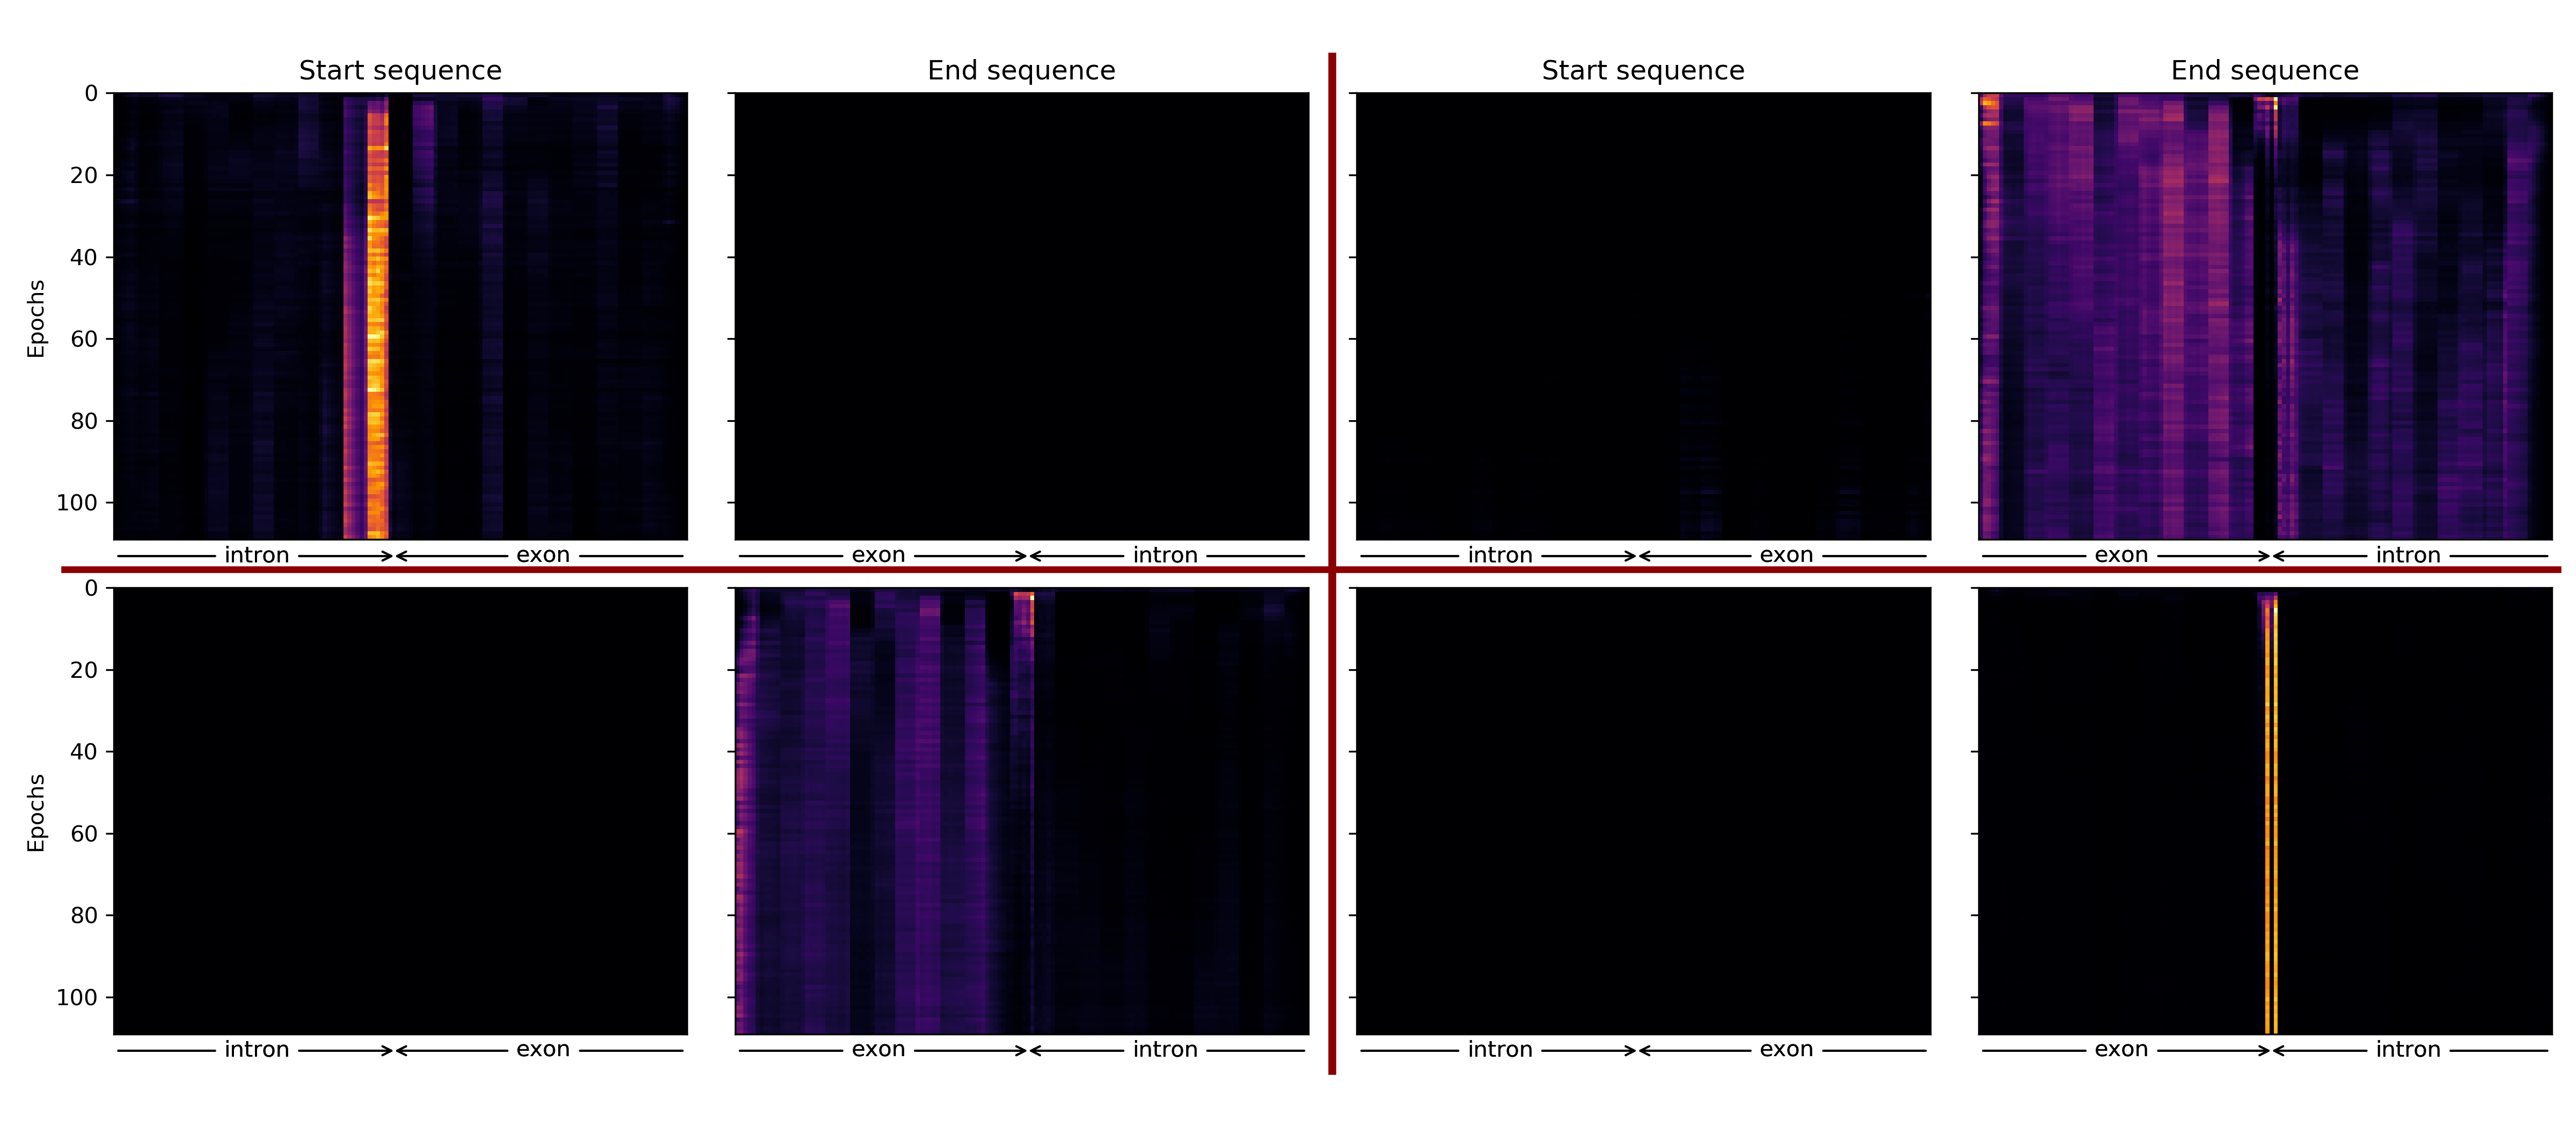
\includegraphics[width=1.3\textwidth]{../visualizations/ch5-results/attention_heatmap.png} 	}
	
	\caption{Each of the four quadrants (marked by the red grid) shows the distribution of the attention weights for a single attention head. The distribution of attention weights is visualized via one heatmap for the start and one heatmap for end sequence, showing how the distribution of attention weights develops during training. The mean distribution of the attention weights over the test set is displayed.}
	\label{fig:attn_heatmap}
	
	
	%	lines idea taken from https://discourse.matplotlib.org/t/horizontal-and-vertical-lines-between-subplots/13540 or powerpoint, https://stackoverflow.com/questions/26084231/draw-a-separator-or-lines-between-subplots?rq=1
\end{figure}

%We visualize to what parts of the input sequence RASC pays attention to in \ref{fig:attn_distribution}. 

%graphics in this section:\\
%- 4x2 heatmaps of mean attention over epochs of all four attention heads\\
%- 1 barchart of final mean attention over mean of all attention heads\\
%- 1+ barcharts for analyzing specific exons

%heatmap analysis:
%\begin{itemize}
%	\item Different attention heads focus on different things, although some overlap
%	\item attention rarely extremely focussed, but honestly can't really tell on this picture
%\end{itemize}

\subsubsection{Heads focus on a single sequence} 
When using a single attention head, the head needs to split its conceptual `focus' over the start and end input sequences. This is not the case for multiple attention heads: here single heads may focus on only one sequence as long as there is at least one attention head which also pays attention to the information in the other sequence. We observe exactly this behaviour in Figure \ref{fig:attention_heatmap}: one of the attention head attends purely to the start sequence and all other attention heads attend purely to the end sequence. Across the 9 cross-validation runs, single attention heads only split their `focus' 7 out of 36 times. None of the trained models only ever pay attention to only a single sequence. This reassures us that the dataset isn't biased such that the model only needs to take information from one sequence into account. 

The sequence which an attention head focusses on generally does not change after the first 5 epochs. Similar observation, that the role of attention heads is decided very early on in training, have also been made in the context of NLP \cite{sixteenheads}.

\subsubsection{What does the model pay attention to?}

\begin{figure}
	\centering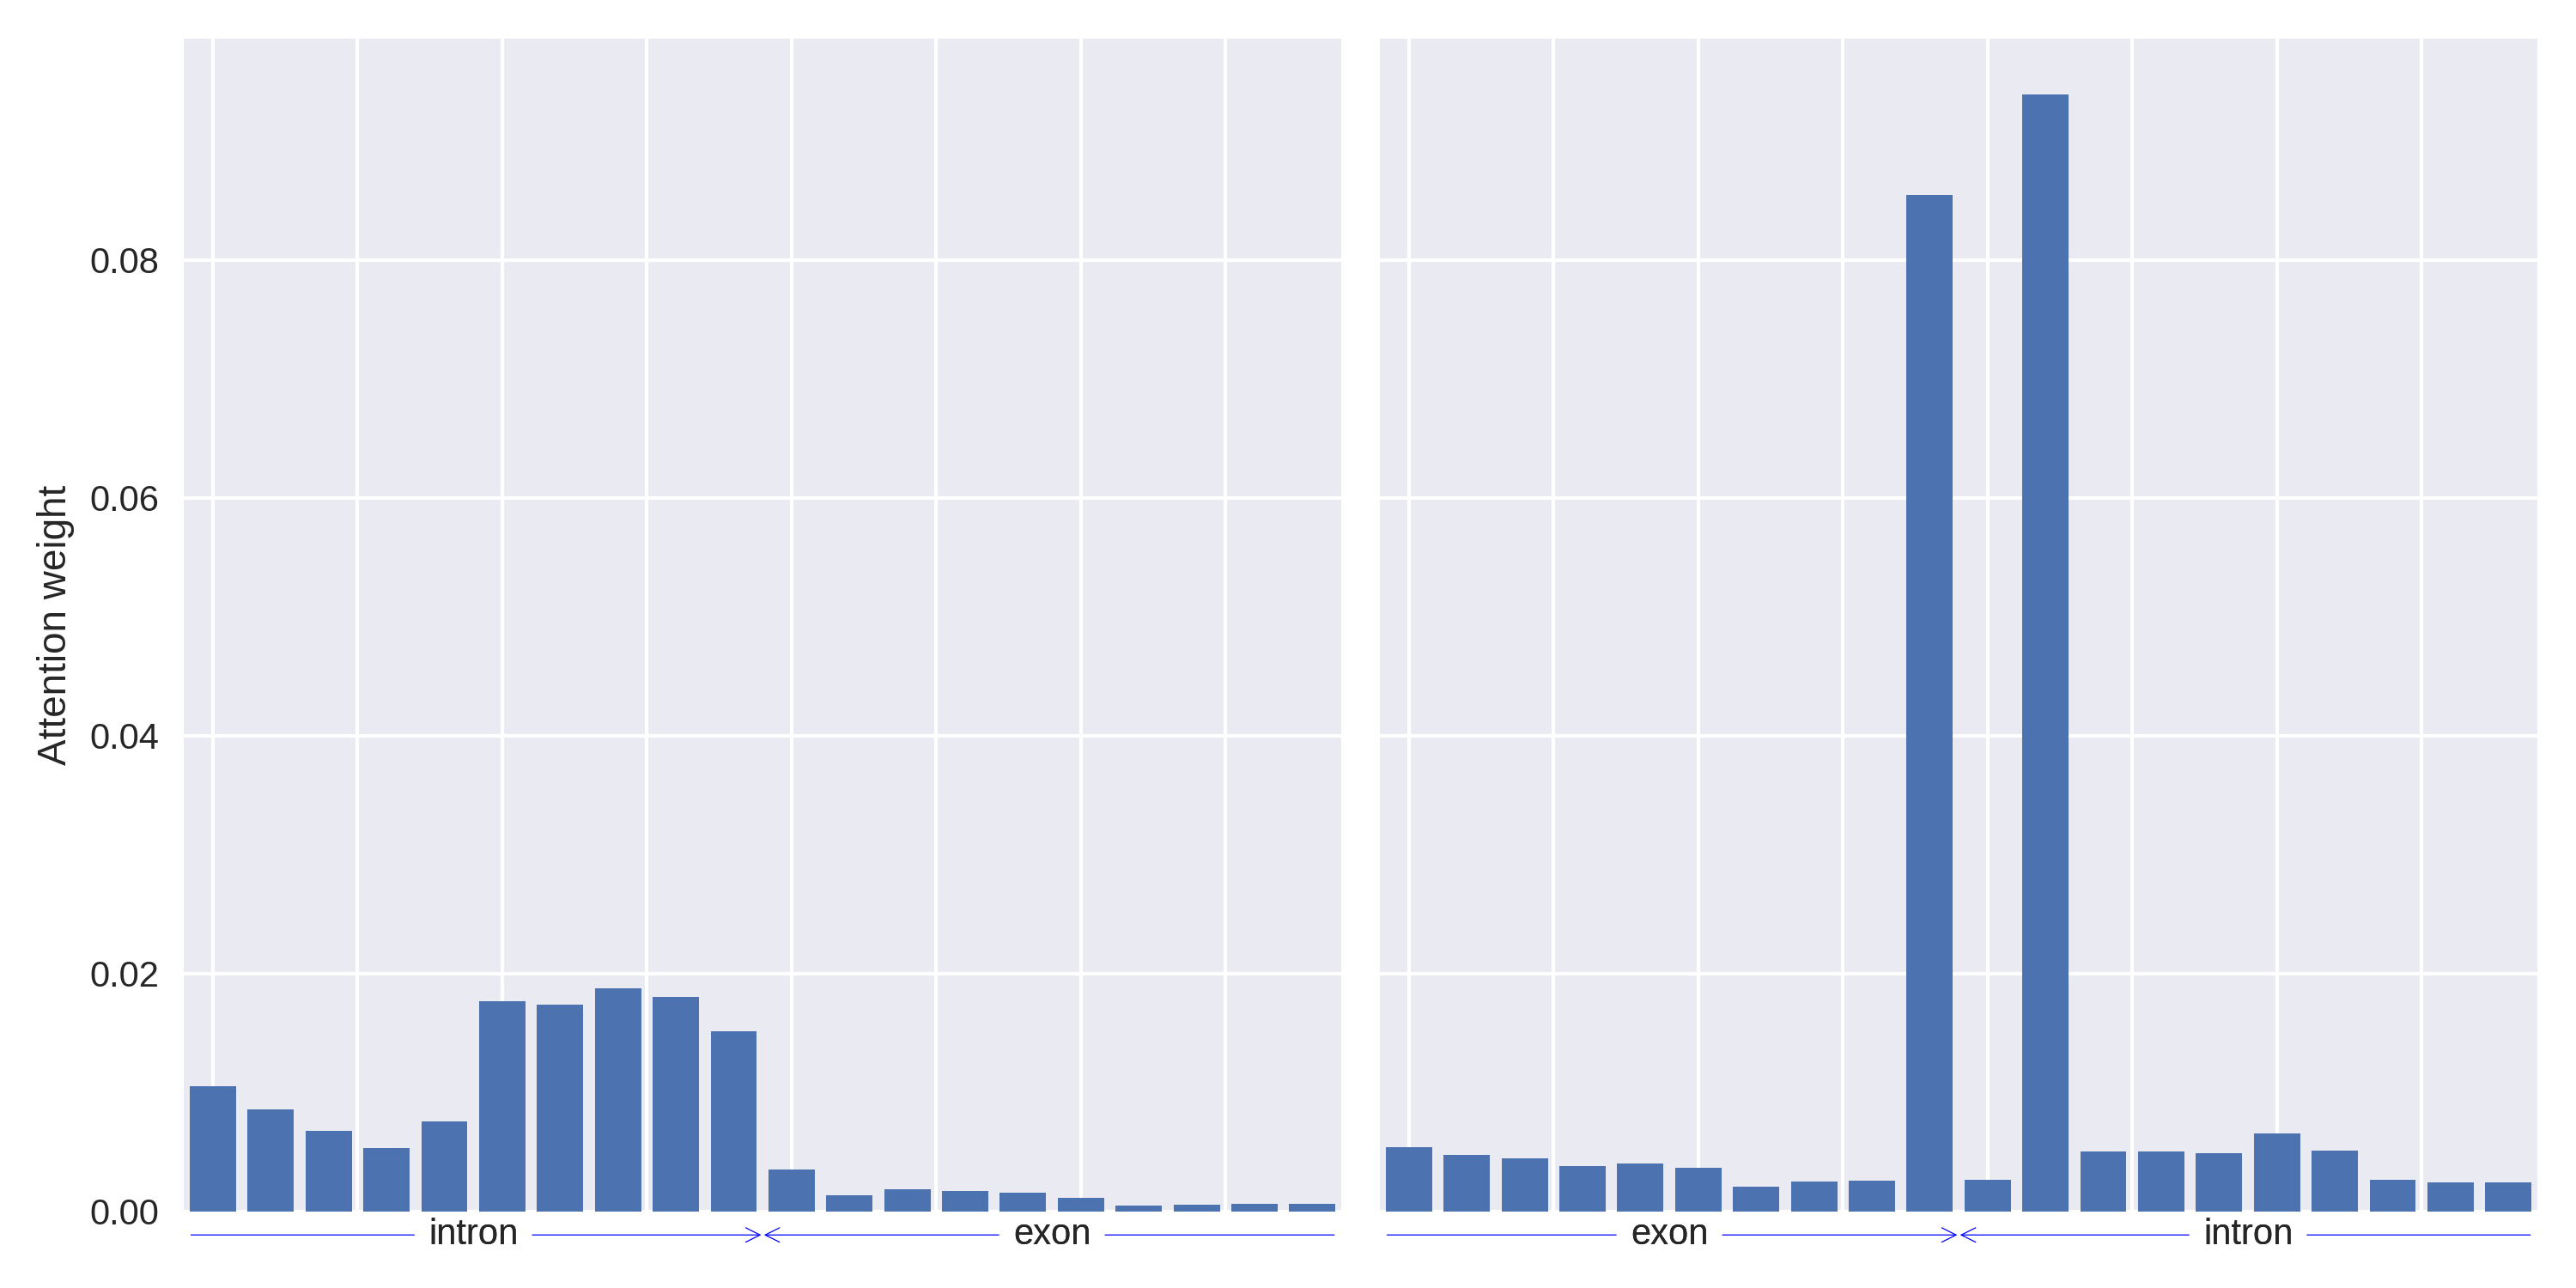
\includegraphics[width=1\textwidth]{../visualizations/ch5-results/mean_attention_barchart_zoomed.png}
	\caption{Mean attention weights averaged over all test samples and all four attention heads. Error bars show the standard deviation between cross-validation runs. }
	\label{fig:mean_attn}
\end{figure}

%\begin{figure}
%	\centering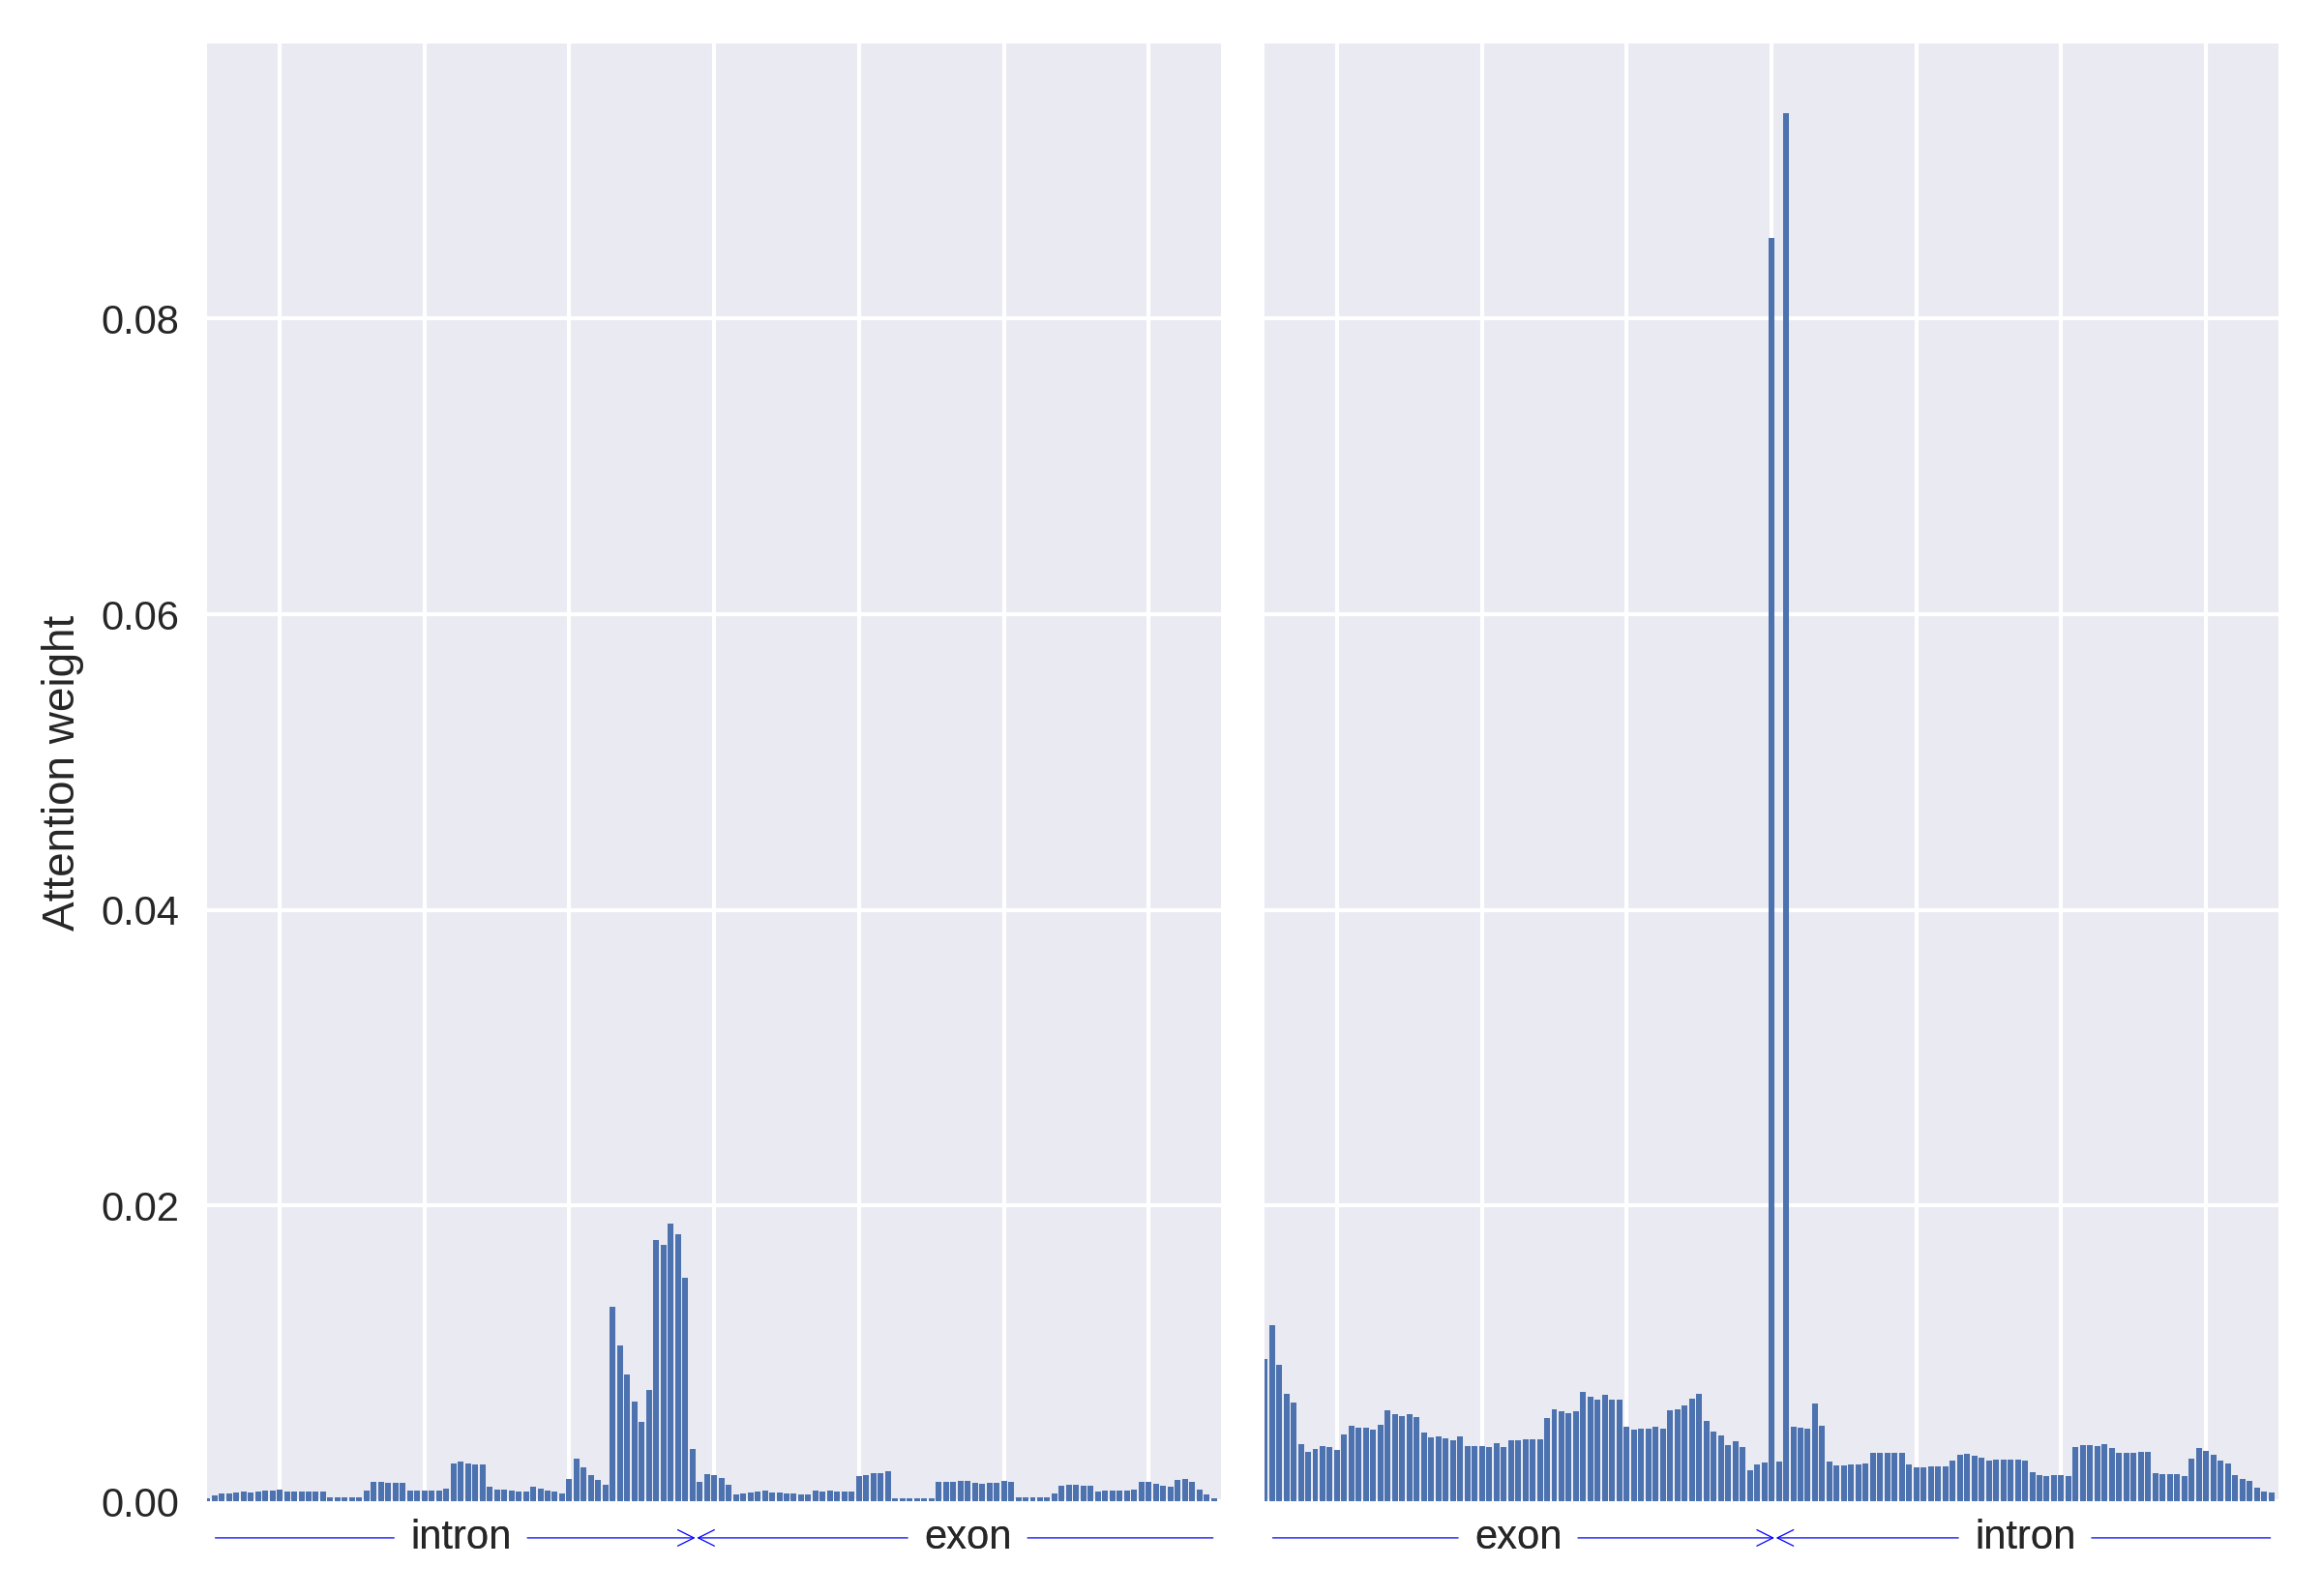
\includegraphics[width=1\textwidth]{../visualizations/ch5-results/mean_attention_barchart.png} 
%	\caption{Mean attention weights averaged over all test samples and all four attention heads. }
%	\label{fig:mean_attn}
%\end{figure}
Averaging the attention weights over all heads over all cross-validation runs at the end of training, we visualize the 20 nucleotides around the exon and intron boundaries in \ref{fig:mean_attn}. The areas around the boundaries are the most attended to parts of the sequences (we provide the attention distribution over the full sequences in the appendix in Figure \ref{app:mean_attn}).
%Figure \ref{fig:mean_attn} shows what part of the input sequence RASC commonly attends to. 
%Clearly, motifs directly around the exon start and exon end are the most attended to. 

% TODO: 84% note

%TODO now this is a job for Liz and Wil
%The bar chart suggests that more total attention is paid to the end, rather than the start sequence. However, this pattern is reversed for other runs of the models and likely just a consequence of three heads focusing on the end sequence in the particular training run which is shown. Additionally, note that the different attention heads might be weighted differently by the unifying matrix $W^O$. 

However, care should be taken when interpreting these results. The attention weights don't directly correspond to the relative importance of each position for multiple reasons: 
\begin{enumerate}[label=(\alph*)]
	\item A position, as displayed in Figure \ref{fig:mean_attn}, contains the information from multiple positions in the sequence because RASC is based on BiLSTM units.
	\item The shown attention weights are a mean between all test set samples and several training runs. Therefore, they don't correspond to the attention weights used by any particular model for any particular training sample. 
	\item The variance between runs is large: generally 20\% of the mean value. A contributing factor is that the attention distribution of the model likely shifts based on which information is encoded in which position. Thus this observation is also related to (a).
	\item The displayed attention weights are a mean between the four attention heads. We know from Section \ref{subsubsec:result_heads} that RASC's performance is similar with only one attention head. Thus, there is likely some redundant overlap between the focus of different heads (e.g. two heads focus on the region close to the exon/intron boundary). Since the overlapping attention is redundant, the overlap is free to shift between runs likely introducing further noise into the attention weights we observe. Additionally, while we averaged the attention weights between heads, RASC unifies them via the learned matrix $W^O$ which might not apply an uniform weighting (e.g. it might assign more weight to heads if they are the only head attenting a particular region). 
\end{enumerate}

Thus, while the results in \ref{fig:mean_attn} can serve to identify a general trend regarding which sequence regions contain the information most relevant to splicing behaviour, they should not be the basis for specific conclusions about the relative importance of specific nucleotide positions. 

If the goal is working towards such an interpretation (based on a deep learning model), a BiLSTM unit should not be used to find representations for the nucleotides. A fully connected-model which does not mix information between positions until the attention layer would be better suited. Additionally, only one attention head should be used. 

Further modifications, which don't require architectural changes include taking the mean attention weights over more cross-validation runs and only visualizing the attention weight for one training sample. Finally, architecture-independent techniques for visualizing the inputs with the greatest impact for a specific prediction could be applied \cite{deeplift}.

%<paragraph about how to go about fixing these errors>
%- fully-connected layer
%- single attention head
%- many runs
%- single test sample 
%
%utility is general trend, but not necessarily accurate finding of most important motifs
%- bilstm so 1nucleotide in graphic <!-> information in one nucleotide
%- variance between runs - see plot
%- it's a mean, i.e., the model doesn't really act like that in practice
%- i took a mean - unifying matrix might do it differently and particular some dimensions in the representation of a particular nucleotide might be weighted differently


%\begin{figure}
%	\centering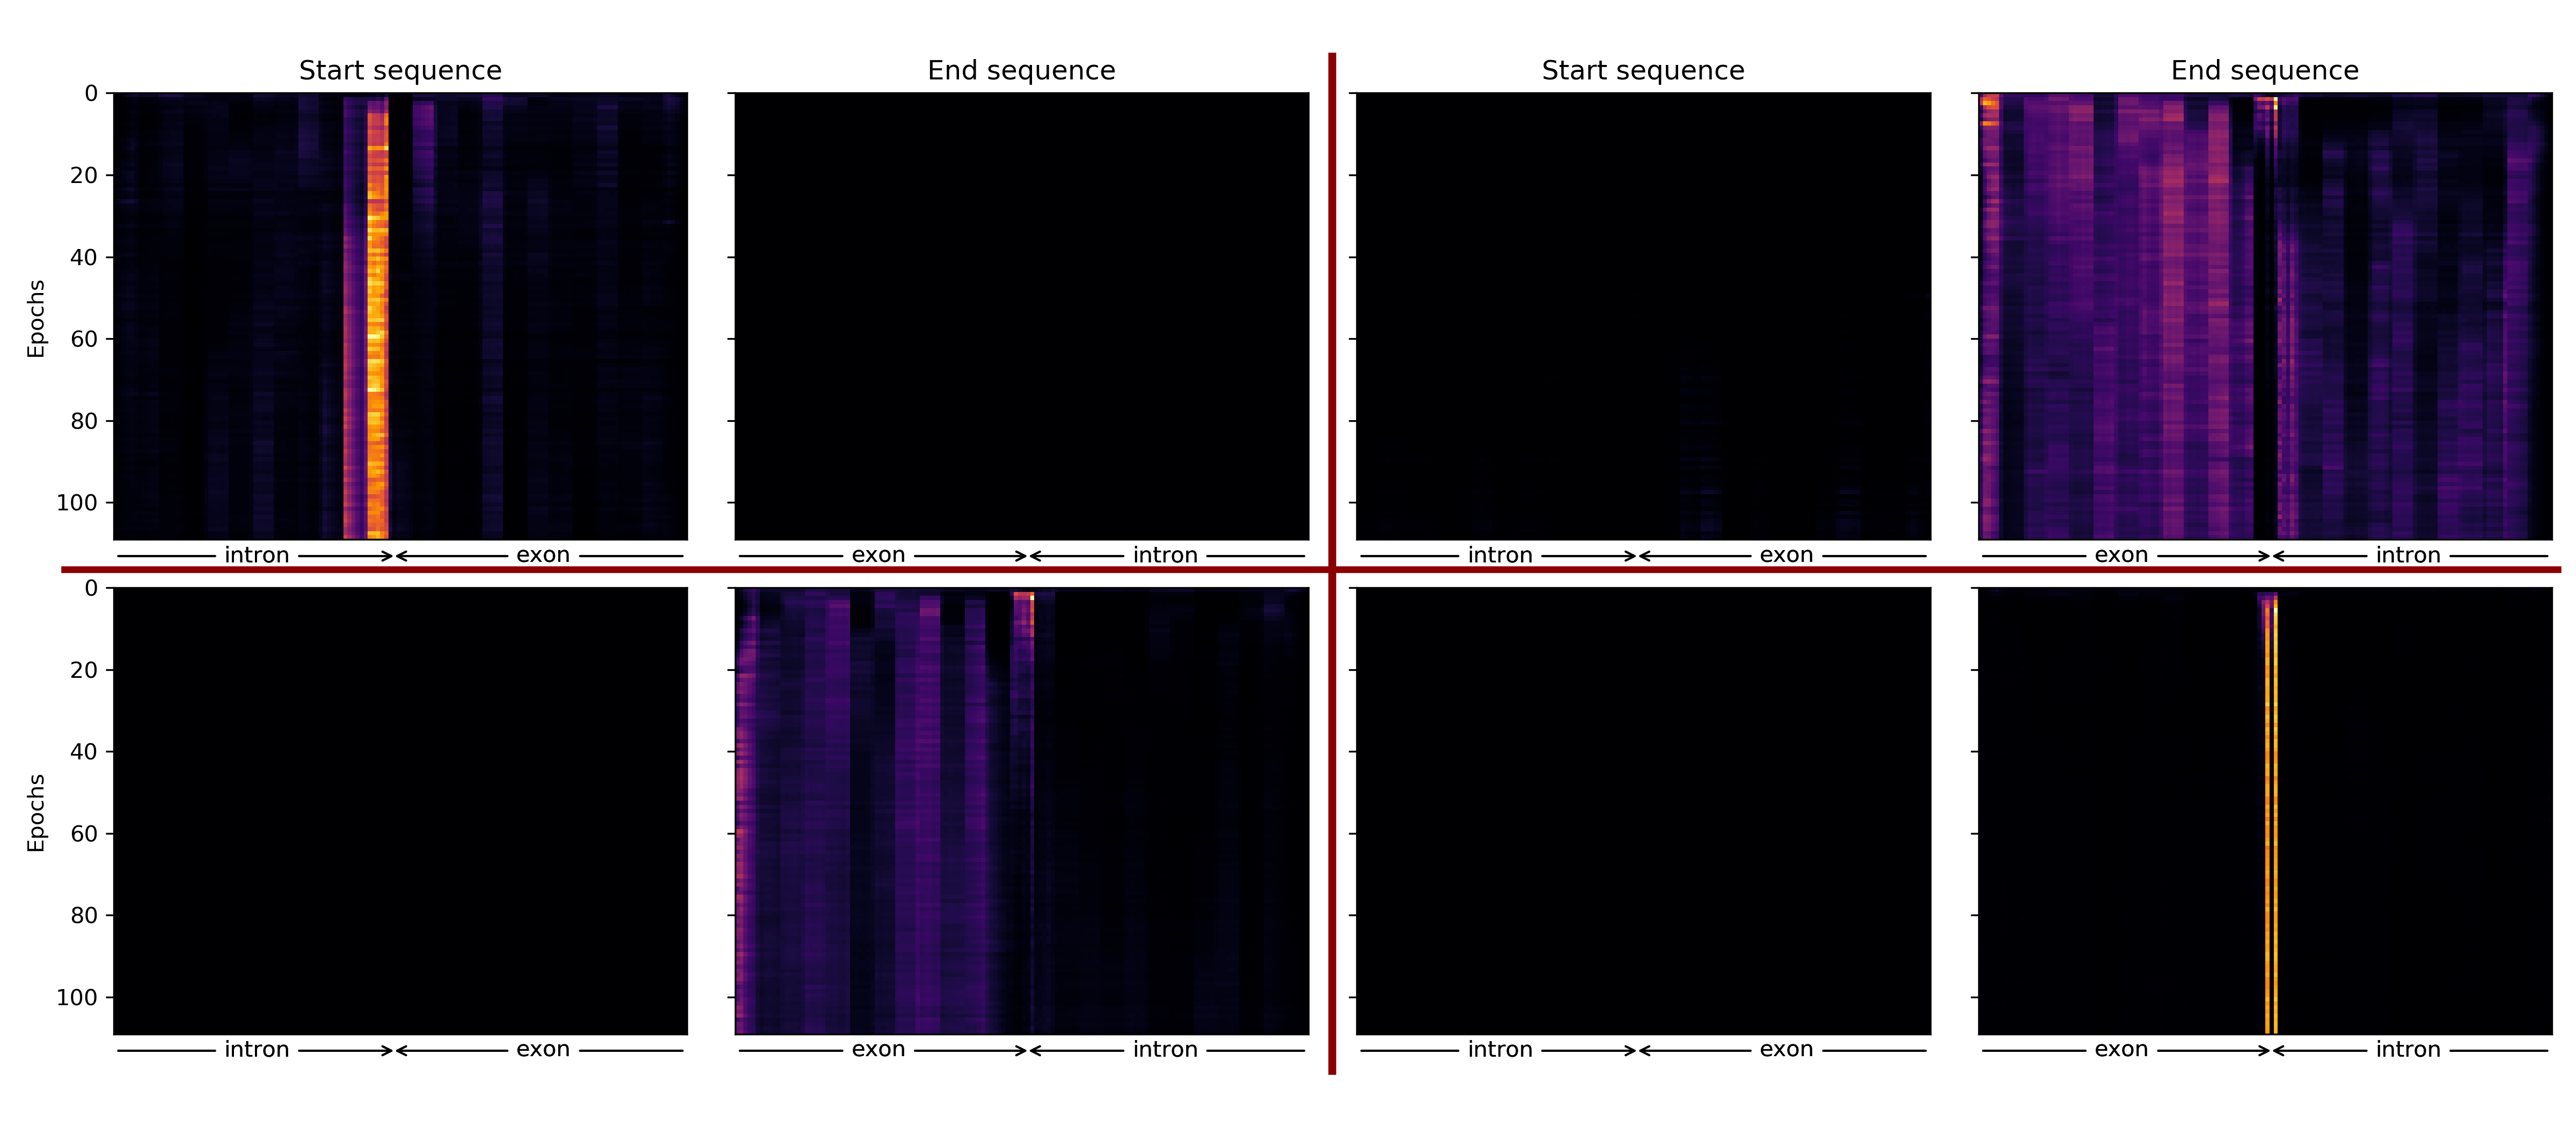
\includegraphics[width=1\textwidth]{../visualizations/ch5-results/attention_heatmap.png} 
%	\caption{Development of attention during training. }
%	\label{fig:attn_heatmap}
%\end{figure}






%attention distribution, proper:
%run id | distribution of heads
%0 | end/end/end/start
%1 | start/end/end/end
%2 | start/start/end/end
%3 | start/start/start/start but then mixed/mixed/mixed/mixed
%4 | end/start/end/start
%5 | start/start/start/mixed
%6 | start/end/start/start (tiny bit mixed 0.8)
%7 | start/end/start/start
%8 | end/mixed/end/mixed (from end/end/end/end at the beginning, switch after like 60 epochs)









%for destruction of EST the following may be interesting: Quantitative comparison of EST libraries requires compensation for systematic biases in cDNA generation

%perhaps mention how older psi regression methods used mouse data but we want human data and that is why we can't use their datasets


%motivation for why classification task was chose and not regression:
%older methods used mouse data
%we reimplement models from regression
%we start off with classification and then move on to regression once we get good enough perforamnce as regression is more challenging
%reasonable to assume that progress in one will also lead to progress in the other

%observation that best performing datasets contain the most samples




\begin{savequote}[8cm]
	
	Oooooh, the weary traveller draws close to the end of the path.
	\qauthor{--- Izaro, Emperor of the Eternal Empire
		%		Cicero's \textit{de Finibus Bonorum et Malorum}
	}
\end{savequote}

\chapter{\label{ch:6-conclusion}Conclusion} % 360
\section{Summary}
This work approached the task of predicting alternative splicing behaviour from a deep learning perspective.
We discussed key challenges which should be addressed when estimating PSI, implemented a method for PSI estimation and constructed splicing quantification datasets based on processing with our PSI estimation method, SUPPA and MAJIQ. We proposed RASC: a novel computational splicing code which is the first to introduce an attention mechanism to splicing quantification and reimplemented the two baselines models DSC and D2V. %from the literature.

Evaluating the models on HEXEvent, we showed that HEXEvent is confounded and that the performance of DSC on HEXEvent can be matched by extremely simple MLPs with two to three orders of magnitudes fewer parameters which use no sequence information. 
Moving to the datasets we constructed, we found that only the HipSci MAJIQ dataset provides data of appropriate quality and quantity. Evaluating RASC on HipSci MAJIQ, RASC outperforms DSC and D2V by at least 15\% each. In further experiments, we showed that RASC generalizes extremely well to different conditions, demonstrated that it has high specificity and gave evidence that RASC also compares favourably to other methods from the literature when regressing PSI. Finally, we showed that the nucleotides around exon and intron boundaries are most attended to by RASC.
\section{Discussion and Future Work}
\subsection{The need for better datasets}
Our work further corroborates 
%the importance and difficulty of constructing datasets of appropriate quality to train Deep Learning models.  
the lack of publically available, standardized datasets suitable for the training of Machine Learning-based splicing codes that was already lamented during the introduction of HEXEvent in 2013 \cite{hexevent}. %We find that there is wide variability between the quality of published data processing methods and datasets.
%As already lamented during the introduction of HEXEvent \cite{hexevent}, 
%There is a dearth of standardized datasets suitable for the training of Machine Learning-based splicing codes. 
The most commonly used dataset to train splicing codes is based on mouse, instead of human, data and not publically made available in an accessible format \cite{jha}. As a result, many papers introducing new splicing codes attempt to reconstruct this dataset \cite{d2vsplicing}, use HEXEvent \cite{dsc} or construct their own dataset ad hoc \cite{cossmo}. This places the additional burden of dataset construction on each author and makes comparisons only indirectly possible or flawed, when implementation differences lead to different versions of the same dataset. %\cite{leung2014} and there is no modern RNA-seq dataset available. 
In contrast, the wide use of standardized, publically available datasets would allow a quicker iteration of ideas and a fair comparison between them. 
%Such datasets have for instance lead to a rapid succession of breakthroughs in Computer Vision and NLP \cite{deeplearning}.
%In contrast, the rapid succession of breakthroughs in Computer Vision and NLP was only possible through the wide use of standardized datasets which allowed a quick iteration of ideas and a fair comparison between them. 
For these reasons, we believe that a concerted effort to construct high-quality, standardized datasets for the training of machine learning, and particular deep learning, splicing codes should be undertaken. We plan to make our HipSci MAJIQ datasets, as well as our code base, publically available as a stepping stone towards this goal.
%We showed that there are still large improvements to be made in the domain of splicing models by applying promising methods from the other application areas of Deep Learning. 

\subsection{Possible improvements to RASC}
While RASC improves upon previous models by a wide margin, there is still scope to improve its prediction accuracy and there are many avenues for future work. 

RASC's predictive power could further be improved by incorporating additional information sources known to affect splicing, like the tissue of an exon or chromatin states \cite{chromatin}. Increasing the amount of sequence information given to RASC is another simple, yet promising idea. 
Futhermore, even hyperparameter tuning may lead to performance improvements since our hyperparameter tuning was limited due to computational constraints. Experiments maxing out the batch size (and stabilizing training) or evaluating different learning rate schedules would be particularly interesting. 


Like all deep learning models, RASC suffers from poor interpretability. While we have taken some first steps towards interpreting RASC by analyzing what parts of a sequence it attends to, a lot more work remains to be done. We discussed changes to RASC's model architecture to make its interpretation more reliable, such as replacing the BiLSTM units and using only one attention head. Further inspiration could be taken from methods exploring the inner workings of Transformer models in NLP \cite{interpretingbert}. General neural network visualization techniques such as DeepLIFT \cite{deeplift} which visualize the relative importance of the inputs for a specific prediction could also be used.
% what input features are the most important for a specific training sample 
%Additionally, methods which visualize what input features are the most important for a specific training sample 
%
%the research efforts that have gone into developing algorithms 
%Alternatively, methods like DeepLIFT \cite{deeplift} which visualize which important features the general techniques to highlight important features for Deep Learning models could be applied \cite{deeplift}. 

With a view to its practical application, adapting RASC for differential splicing prediction is a promising avenue of future research. Here the existing tool MAJIQ could be exploited to generate a dataset for splicing changes between conditions. A model capable of predicting the impact of genetic variations on splicing would be extremely valuable for the emerging field of personalized medicine.



%In conclusion, we showed 

%say that data processing was the most time-consuming task due to the novelty of the task and no standard datasets available
%
%- proper dataset construction very challenging with varying quality of available tools and datasets; only one of the four datasets proved sufficient
%- across all datasets, the newly introduced splicing code RASC generally performs best.
%
%future work: differential splicing, link other datasets
%future work could also be using gtex data directly perhaps? 
%differential splicing for sure
% 
%future work: data augmentation as performance dropped 2-3\% once I removed 10%
%easy extension would check whether more context than 140 nucleotides help
%continuous splicing prediction; more than 140 nt probably desirable 
%
%
%We make our dataset publicly available; related to talking about publishing this research in general 

%% APPENDICES %% 
% Starts lettered appendices, adds a heading in table of contents, and adds a
%    page that just says "Appendices" to signal the end of your main text.
\startappendices
% Add or remove any appendices you'd like here:
\begin{savequote}[8cm]
\textlatin{Cor animalium, fundamentum e\longs t vitæ, princeps omnium, Microco\longs mi Sol, a quo omnis vegetatio dependet, vigor omnis \& robur emanat.}

The heart of animals is the foundation of their life, the sovereign of everything within them, the sun of their microcosm, that upon which all growth depends, from which all power proceeds.
  \qauthor{--- William Harvey %\cite{harvey_exercitatio_1628}
  }
\end{savequote}

\chapter{\label{app:appendix}Appendix}

\minitoc


\section{Accession Numbers of HipSci data} \label{app:hipsci_celllines}
The ENA Accession Numbers of the 25 biological replicates belonging to sensory neuron cell lines \cite{ipscneurons} are ERR177-: 
5544, 5551, 5552, 5554, 5594. 5595, 5596, 5598, 5600, 5601, 5631, 5634, 5637, 5638, 5640, 5641, 5643, 5644, 5684, 5685, 5686, 5687, 5688, 5689, 5693.
While all of these were used in MAJIQ Builder process (and thus contributed to the constitutive exons), only the sample with Accession Number ERR1775544 was used with the MAJIQ PSI step (and thus determined the alternatively spliced exons). 

The ENA Accession Numbers of the 20 biological replicates belonging to undifferentiated iPSC cell lines \cite{hipsci} are ERR-: 
914342, 946968, 946976, 946983, 946984, 946990, 946992, 946994, 947011, 1203463, 1243454, 1274914, 1274917, 1724696, 1724699, 1743789, 2039345, 2039336, 2278244 2278245.
Similarly, all of the above biological replicates were used in the MAJIQ Builder process. Only the samples with Accession Numbers ERR946992, ERR946984 (same cell type and donor as ERR946984, but different cell line), and ERR946968 (same cell type, but different donor) were used with MAJIQ PSI. 
%bezi1, 2 
%lexy 2
%25 biological replicates:
%ERR1775544 - 0 
%ERR1775551 - 1
%ERR1775552 - 2
%ERR1775553 - 3
%ERR1775554 - 4
%---
%ERR1775594 - 5
%ERR1775595 - 6
%ERR1775596 - 7
%ERR1775598 - 8
%ERR1775600 - 9
%ERR1775601 - 10
%--- 
%ERR1775631 - 11
%ERR1775634 - 12
%ERR1775637 - 13
%ERR1775638 - 14
%ERR1775640 - 15
%ERR1775641 - 16
%ERR1775643 - 17
%ERR1775644 - 18
%---
%ERR1775684 - 19
%ERR1775685 - 20
%ERR1775686 - 21
%ERR1775687 - 22
%ERR1775688 - 23
%ERR1775689 - 24
%ERR1775693 - 25
%
%20:
%bezi1,bezi2,eipl1,eipl2,iisa1,iisa2,kolf1,kolf2,lexy1,lexy2,rozh1,rozh2,zapk1,zapk2,aion1,aion2,aoxv1,aoxv2,bimq1,bimq2
%
%ERR914342
%
%ERR946968
%ERR946976
%ERR946983
%ERR946984
%ERR946990
%ERR946992
%ERR946994
%
%ERR947011
%
%ERR1203463
%ERR1243454
%ERR1274914
%ERR1274917
%
%ERR1724696
%ERR1724699
%ERR1743789
%
%ERR2039345
%ERR2039336
%
%ERR2278244
%ERR2278245

%unsorited, but paired: 
%ERR946992
%ERR946984
%
%ERR914342
%ERR1274917
%
%ERR1243454
%ERR946994
%
%ERR1203463
%ERR946983
%
%ERR946990
%ERR946968
%
%ERR947011
%ERR946976
%
%ERR1724696
%ERR1274914
%
%ERR1724699
%ERR1743789
%
%ERR2039345
%ERR2039336
%
%ERR2278244
%ERR2278245

\section{Additional Doc2Vec training details} \label{app:d2v}

\begin{table}[h!]
	\centering
	\begin{tabular}{ c c c  c c c} 
		\hline
		%   & configuration & & performance & \\
		Training method & DM \\
		Embedding dimensions & 100 \\
		Corpus & Human Genome GRCh38 \\
		Window size & 5\\
		Minimum count & 5\\
		Negative sampling & 5\\
		Epochs & 5\\
		
		\hline
	\end{tabular}
	\caption{Exact hyperparameters used for training Doc2Vec model.
	}
	\label{table:d2vparams}
\end{table}

The hyperparameters used during pre-training are given in table \ref{table:d2vparams}. Except for the number of epochs, these are the same as in the baseline paper \cite{d2vsplicing}. We reduced the number of epochs from 20 to 5, as initial tests showed no performance difference between these two values. However, while \cite{d2vsplicing} don't mention what Doc2Vec implementation they use, almost all of these parameters are the same as the default parameters from the gensim library. Therefore, we believe that these parameters weren't fine-tuned very intensively. 

Two hyperparameters, not yet introduced, are mentioned in Table \ref{table:d2vparams}. Although these hyperparameters aren't very impactful when training on genomic data (as the vocabulary only consists of 64 words), we mention them for completeness (as they are also mentioned in \cite{d2vsplicing}):
\begin{itemize}
	\item The minimum count parameters eliminates all words which occur fewer than the minumum amount from the corpus. Infrequent words don't have enough examples to allow the model to learn a good representation of them. Additionally, while the individual words might uncommon, there might be a lot of them, making it computationally expensive to keep them.
	
	\item Negative sampling \cite{w2v2} 
	is a technique to reduce the computational cost of backpropagating the gradient updates. The size of the weights in the Word2Vec or Doc2Vec can be easily reach millions of learnable weights with a medium sized vocabulary: for 10,000 words in the vocabulary and 300-dimensional embedding, the matrix representing the hidden weights already has 3 million weights. This makes backpropagation expensive as all of these weights need to be updated in every step. \\
	When negative sampling is enabled, by default only the weights connected to the word tne network should predict will be updated via backpropagation. Additionally, a certain number of negative samples, words which the network shouldn't predict, are randomly chosen and their weights updated too. This dramatically reduces the computational cost of backpropagating the gradient updates, since only the weights of very few words in the vocabulary are updated. 
\end{itemize}



 
%TODO do I even need to explain these if I just use the default gensim option either way?
% ---> could just explain sub-sampling too if I have time cause more text and I sound smarter
%http://mccormickml.com/2017/01/11/word2vec-tutorial-part-2-negative-sampling/




%%%%% REFERENCES

% JEM: Quote for the top of references (just like a chapter quote if you're using them).  Comment to skip.
\begin{savequote}[8cm]
The first kind of intellectual and artistic personality belongs to the hedgehogs, the second to the foxes \dots
  \qauthor{--- Sir Isaiah Berlin \cite{berlin_hedgehog_2013}}
\end{savequote}

\setlength{\baselineskip}{0pt} % JEM: Single-space References

{\renewcommand*\MakeUppercase[1]{#1}%
\printbibliography[heading=bibintoc,title={\bibtitle}]}

\printbibliography
%\bibliographystyle{plain}
%
%\bibliography{references}


\end{document}
